% YYY: Fix d bar
% YYY: ``abslute''
% YYY: Hong only for connected graphs?
%
%
% UCSD Doctoral Dissertation Template
% -----------------------------------
% http://ucsd-thesis.googlecode.com
%
%
% ----------------------------------------------------------------------
% WARNING: 
%
%   This template has not endorced by OGS or any other official entity.
%   The official formatting guide can be obtained from OGS.
%   It can be found on the web here:
%   http://ogs.ucsd.edu/AcademicAffairs/Documents/Dissertations_Theses_Formatting_Manual.pdf
%
%   No guaranty is made that this LaTeX class conforms to the official UCSD guidelines.
%   Make sure that you check the final document against the Formatting Manual.
%  
%   That being said, this class has been routinely used for successful 
%   publication of doctoral theses.  
%
%   The ucsd.cls class files are only valid for doctoral dissertations.
%
%
% ----------------------------------------------------------------------
% GETTING STARTED:
%
%   Lots of information can be found on the project wiki:
%   http://code.google.com/p/ucsd-thesis/wiki/GettingStarted
%
%
%   To make a pdf from this template use the command:
%     pdflatex template
%
%
%   To get started please read the comments in this template file 
%   and make changes as appropriate.
%
%   If you successfully submit a thesis with this package please let us
%   know.
%
%
% ----------------------------------------------------------------------
% KNOWN ISSUES:
%
%   Currently only the 12pt size conforms to the UCSD requirements.
%   The 10pt and 11pt options make the footnote fonts too small.
%
%
% ----------------------------------------------------------------------
% HELP/CONTACT:
%
%   If you need help try the ucsd-thesis google group:
%   http://groups.google.com/group/ucsd-thesis
%
%
% ----------------------------------------------------------------------
% BUGS:
%
%   Please report all bugs at:
%   http://code.google.com/p/ucsd-thesis/issues/list
%
%
% ----------------------------------------------------------------------
% More control of the formatting of your thesis can be achieved through
% modifications of the included LaTeX class files:
%
%   * ucsd.cls    -- Class file
%   * uct10.clo   -- Configuration files for font sizes 10pt, 11pt, 12pt
%     uct11.clo                            
%     uct12.clo
%
% ----------------------------------------------------------------------



% Setup the documentclass 
% default options: 12pt, oneside, final
%
% fonts: 10pt, 11pt, 12pt -- are valid for UCSD dissertations.
% sides: oneside, twoside -- note that two-sided theses are not accepted 
%                            by OGS.
% mode: draft, final      -- draft mode switches to single spacing, 
%                            removes hyperlinks, and places a black box
%                            at every overfull hbox (check these before
%                            submission).
% chapterheads            -- Include this if you want your chapters to read:
%                              Chapter 1
%                              Title of Chapter
%
%                            instead of
%                              1 Title of Chapter
\documentclass[12pt,chapterheads]{ucsd}



% Include all packages you need here.  
% Some standard options are suggested below.
%
% See the project wiki for information on how to use 
% these packages. Other useful packages are also listed there.
%
%   http://code.google.com/p/ucsd-thesis/wiki/GettingStarted



%% AMS PACKAGES - Chances are you will want some or all 
%    of these if writing a dissertation that includes equations.
%  \usepackage{amsmath, amscd, amssymb, amsthm}

%% GRAPHICX - This is the standard package for 
%    including graphics for latex/pdflatex.
\usepackage{scrextend}
\usepackage{pslatex}
\usepackage{graphicx}
\usepackage{tikz}
\usepackage{mathtools}
\usepackage{amssymb}
\usepackage{bbm}
\usepackage{amsthm}
\usepackage{subcaption}
\usepackage{epstopdf}

\usetikzlibrary{calc}

\newtheorem{theorem}{Theorem}[section]
\newtheorem{lemma}[theorem]{Lemma}
\newtheorem{prop}[theorem]{Proposition}
\newtheorem{corollary}[theorem]{Corollary}
\newcommand{\vol}{{\rm vol}}
\newcommand{\ignore}[1]{}

\newtheorem{proposition}[theorem]{Proposition}


%% CAPTION
% This overrides some of the ugliness in ucsd.cls and
% allows the text to be double-spaced while letting figures,
% tables, and footnotes to be single-spaced--all OGS requirements.
% NOTE: Must appear after graphics and ams math
\makeatletter
\gdef\@ptsize{2}% 12pt documents
\let\@currsize\normalsize
\makeatother
\usepackage{setspace}
\doublespace
\usepackage[font=small, width=0.9\textwidth]{caption}

%% SUBFIG - Use this to place multiple images in a
%    single figure.  Subfig will handle placement and
%    proper captioning (e.g. Figure 1.2(a))
% \usepackage{subfig}

%% TIMES FONT - replacements for Computer Modern
%%   This package will replace the default font with a
%%   Times-Roman font with math support.
% \usepackage[T1]{fontenc}
% \usepackage{mathptmx}

%% INDEX
%   Uncomment the following two lines to create an index: 
% \usepackage{makeidx}
% \makeindex
%   You will need to uncomment the \printindex line near the
%   bibliography to display the index.  Use the command
% \index{keyword} 
%   within the text to create an entry in the index for keyword.
%   To compile a LaTeX document with an index the 'makeindex'
%   command will need to be run.  See the wiki for more details.

%% HYPERLINKS
%   To create a PDF with hyperlinks, you need to include the hyperref package.
%   THIS HAS TO BE THE LAST PACKAGE INCLUDED!
%   Note that the options plainpages=false and pdfpagelabels exist
%   to fix indexing associated with having both (ii) and (2) as pages.
%   Also, all links must be black according to OGS.
%   See: http://www.tex.ac.uk/cgi-bin/texfaq2html?label=hyperdupdest
%   Note: This may not work correctly with all DVI viewers (i.e. Yap breaks).
%   NOTE: hyperref will NOT work in draft mode, as noted above.
% \usepackage[colorlinks=true, pdfstartview=FitV, 
%             linkcolor=black, citecolor=black, 
%             urlcolor=black, plainpages=false,
%             pdfpagelabels]{hyperref}
% \hypersetup{ pdfauthor = {Your Name Here}, 
%              pdftitle = {The Title of The Dissertation}, 
%              pdfkeywords = {Keywords for Searching}, 
%              pdfcreator = {pdfLaTeX with hyperref package}, 
%              pdfproducer = {pdfLaTeX} }
% \urlstyle{same}
% \usepackage{bookmark}


%% CITATIONS
% Sets citation format
% and fixes up citations madness
\usepackage{microtype}  % avoids citations that hang into the margin


%% FOOTNOTE-MAGIC
% Enables footnotes in tables, re-referencing the same footnote multiple times.
\usepackage{footnote}
\makesavenoteenv{tabular}
\makesavenoteenv{table}


%% TABLE FORMATTING MADNESS
% Enable all sorts of fun table tricks
\usepackage{rotating}  % Enables the sideways environment (NCPW)
\usepackage{array}  % Enables "m" tabular environment http://ctan.org/pkg/array
\usepackage{booktabs}  % Enables \toprule  http://ctan.org/pkg/array



\begin{document}

%% FRONT MATTER
%
%  All of the front matter.
%  This includes the title, degree, dedication, vita, abstract, etc..
%  Modify the file template_frontmatter.tex to change these pages.
%
%
% UCSD Doctoral Dissertation Template
% -----------------------------------
% http://ucsd-thesis.googlecode.com
%
%


%% REQUIRED FIELDS -- Replace with the values appropriate to you

% No symbols, formulas, superscripts, or Greek letters are allowed
% in your title.
\title{Extremal Spectral Invariants and the Spectral Gap of Reversal Graphs}

\author{Robin Joshua Tobin}
\degreeyear{\the\year}

% Master's Degree theses will NOT be formatted properly with this file.
\degreetitle{Doctor of Philosophy}

\field{Mathematics}
%\specialization{Graph theory}  % If you have a specialization, add it here

\chair{Professor Fan Chung Graham}
% Uncomment the next line iff you have a Co-Chair
\cochair{Professor Jacques Verstra\"{e}te}
%
% Or, uncomment the next line iff you have two equal Co-Chairs.
%\cochairs{Professor Chair Masterish}{Professor Chair Masterish}

%  The rest of the committee members  must be alphabetized by last name.
\othermembers{
Professor Ron Graham\\
Professor Ramamohan Paturi\\
Professor Jeffrey Remmel\\
}
\numberofmembers{5} % |chair| + |cochair| + |othermembers|


%% START THE FRONTMATTER
%
\begin{frontmatter}

%% TITLE PAGES
%
%  This command generates the title, copyright, and signature pages.
%
\makefrontmatter

%% DEDICATION
%
%  You have three choices here:
%    1. Use the ``dedication'' environment.
%       Put in the text you want, and everything will be formated for
%       you. You'll get a perfectly respectable dedication page.
%
%
%    2. Use the ``mydedication'' environment.  If you don't like the
%       formatting of option 1, use this environment and format things
%       however you wish.
%
%    3. If you don't want a dedication, it's not required.
%
%
%\begin{dedication}
%  To two, the loneliest number since the number one.
%\end{dedication}


% \begin{mydedication} % You are responsible for formatting here.
%   \vspace{1in}
%   \begin{flushleft}
% 	To me.
%   \end{flushleft}
%
%   \vspace{2in}
%   \begin{center}
% 	And you.
%   \end{center}
%
%   \vspace{2in}
%   \begin{flushright}
% 	Which equals us.
%   \end{flushright}
% \end{mydedication}



%% EPIGRAPH
%
%  The same choices that applied to the dedication apply here.
%
%\begin{epigraph} % The style file will position the text for you.
%  \emph{A careful quotation\\
%  conveys brilliance.}\\
%  ---Smarty Pants
%\end{epigraph}

% \begin{myepigraph} % You position the text yourself.
%   \vfil
%   \begin{center}
%     {\bf Think! It ain't illegal yet.}
%
% 	\emph{---George Clinton}
%   \end{center}
% \end{myepigraph}


%% SETUP THE TABLE OF CONTENTS
%
\tableofcontents
\listoffigures  % Comment if you don't have any figures
\listoftables   % Comment if you don't have any tables



%% ACKNOWLEDGEMENTS
%
%  While technically optional, you probably have someone to thank.
%  Also, a paragraph acknowledging all coauthors and publishers (if
%  you have any) is required in the acknowledgements page and as the
%  last paragraph of text at the end of each respective chapter. See
%  the OGS Formatting Manual for more information.
%
\begin{acknowledgements}

Chapters 2 and 3 are based on the papers ``Three conjectures in extremal spectral graph theory'',
 \cite{TaitTobin2017}, to appear in \textit{Journal of Combinatorial Theory, Series B},
 and ``Characterizing graphs of maximum principal ratio'', submitted to
 \textit{Electronic Journal of Linear Algebra} \cite{TaitTobin2015},
 both written jointly with Michael Tait.
Chapter 4 is based on the paper ``The Spectral Gap of Graphs Arising from Substring Reversals'',
submitted to \textit{Journal of Combinatorics}, written jointly with Fan Chung.

\end{acknowledgements}


%% VITA
%
%  A brief vita is required in a doctoral thesis. See the OGS
%  Formatting Manual for more information.
%
\begin{vitapage}
\begin{vita}
  \item[2011] B.~A. in Mathematics, TODO
  \item[2013] M.~A. in Mathematics, TODO
  \item[2017] Ph.~D. in Mathematics, University of California, San Diego
\end{vita}
%\begin{publications}
%  \item Your Name, ``A Simple Proof Of The Riemann Hypothesis'', \emph{Annals of Math}, 314, 2007.
%  \item Your Name, Euclid, ``There Are Lots Of Prime Numbers'', \emph{Journal of Primes}, 1, 300 B.C.
%\end{publications}
\end{vitapage}


%% ABSTRACT
%
%  Doctoral dissertation abstracts should not exceed 350 words.
%   The abstract may continue to a second page if necessary.
%
\begin{abstract}
 We address several problems in spectral graph theory, with a common theme of
 optimizing or computing a spectral graph invariant, such as the spectral radius or
 spectral gap, over some family of graphs.  In particular, we study
 measures of graph irregularity, we bound the adjacency spectral radius
 over all outerplanar and planar graphs, and finally we determine the spectral
 gap of reversal graphs and a family of graphs that generalize the
 prefix reversal graph.


 Firstly we study two measures of graph irregularity, the principal ratio and the
 difference between the spectral radius of the adjacency matrix and the average
 degree.  For the principal ratio, we show that when the
 the graphs which maximize this
 statistic are the \textit{kite graphs}, which are a clique with a pendant path,
 when the number of vertices is sufficiently large.
 This answers a conjecture of Cioab\u{a} and Gregory.  For the second graph
 irregularity measure, we show that the graphs which maximize it are
 \textit{pineapple graphs}, answering a conjecture of Aouchciche et. al.


 Secondly we investigate the maximum spectral radius of the adjacency matrix, over
 all graphs on $n$ vertices within certain well-known graph families.
 Our main result is showing that the planar graph on $n$ vertices with maximal adjacency
 spectral radius is the join $P_2 + P_{n-2}$, when $n$ is sufficiently large.  This
 was conjectured independently by Boots and Royle.  Additionally, we
 identify the outerplanar graph with maximal spectral radius, answering a conjecture
 of Cvetkovi\`{c} and Rowlinson.


 Finally, we determine the spectral gap of various Cayley graphs of the symmetric group
 $S_n$, which arise in the context of subtring reversals.  This includes an elementary
 proof that the prefix reversal (or \textit{pancake flipping} graph) has spectral
 gap one, originally proved via representation theory by Cesi.  We generalize this
 by showing that a large family of related graphs all have unit spectral gap.

\end{abstract}


\end{frontmatter}






%% DISSERTATION

% A common strategy here is to include files for each of the chapters. I.e.,
% Place the chapters is separate files: 
%   chapter1.tex, chapter2.tex
% Then use the commands:
%   \chapter{Introduction}

\section{Preliminaries}

\section{Spectral Graph Theory}

\subsection{Fundamentals of Linear Algebra}

\subsection{Matrices Associated to Graphs}

\subsection{Graph Coverings and Projections}

\section{Overview of Results}

%\section{A section}
Lorem ipsum dolor sit amet, consectetuer adipiscing elit. Nulla odio
sem, bibendum ut, aliquam ac, facilisis id, tellus. Nam posuere pede
sit amet ipsum. Etiam dolor. In sodales eros quis pede.  Quisque sed
nulla et ligula vulputate lacinia. In venenatis, ligula id semper
feugiat, ligula odio adipiscing libero, eget mollis nunc erat id orci.
Nullam ante dolor, rutrum eget, vestibulum euismod, pulvinar at, nibh.
In sapien. Quisque ut arcu. Suspendisse potenti. Cras consequat cursus
nulla.

%\subsection{A Figure Example}
\label{ssec:figure_example}

%This subsection shows a sample figure.

%\begin{figure}[h] 
%  \centering
%  \includegraphics[width=0.5\textwidth]{sandiego}
%  \caption[Short figure caption (must be \protect{$< 4$} lines in the list of figures)]{A picture of San Diego.  Note that figures must be on their own line (no neighboring text) and captions must be single-sp%aced and appear \protect\textit{below} the figure.  Captions can be as long as you want, but if they are longer than 4 lines in the list of figures, you must provide a short figure caption.\index{SanDiego}} 
%  \label{fig:sandiego}
%\end{figure}

%\subsection{A Table Example}

While in Section \ref{ssec:figure_example} Figure \ref{fig:sandiego} we had a majestic figure, here we provide a crazy table example.


%%%% TABLE 1 %%%%
\vspace{0.25in}
\begin{table}[!ht]
\caption[Short figure caption (must be \protect{$< 4$} lines in the list of tables)]{A table of when I get hungry.  Note that tables must be on their own line (no neighboring text) and captions must be single-spaced and appear \protect\textit{above} the table.  Captions can be as long as you want, but if they are longer than 4 lines in the list of figures, you must provide a short figure caption.}

\vspace{-0.25in}
\begin{center}
\begin{tabular}{|p{1in}|p{2in}|p{3in}|}

\hline
Time of day & Hunger Level & Preferred Food \\

\hline
8am & high & IHOP (French Toast) \\

\hline
noon & medium & Croutons (Tomato Basil Soup \& Granny Smith Chicken Salad) \\

\hline
5pm & high & Bombay Coast (Saag Paneer) or Hi Thai (Pad See Ew) \\

\hline
8pm & medium & Yogurt World (froyo!) \\

\hline
\end{tabular}
\end{center}
\label{tab:analysis3}
\end{table}



%   \chapter{Measures of Graph Irregularity}
\section{Introduction}

A \textit{measure of graph irregularity} is a  statistics that quantifies how far a graph is
from being regular.  The choice of the word ``measure'' is slightly unfortunate due to its
more common usage in mathematics, but this is the phrase that has been used repeatedly in the
literature, and so we adopt it here.  Many different such statistics have been proposed.
There is the \textit{irregularity of a graph} as defined by Albertson \cite{Albertson1997},
\[ \textrm{irr}(G) = \sum_{(u,v) \in E(G)} \left| d_u - d_v \right| .\]
A variant of this that depends only on the degree sequence of a graph,
the \textit{total irregularity}, was introduced by Abdo et. al. \cite{Abdo2014},
\[ \textrm{irr}_{\textrm{it}}(G) = \frac{1}{2} \sum_{u \in V(G)} \sum_{v \in V(G)} \left| d_u - d_v\right|\]
Another irregularity measure that does depends only on the degree sequence is given by the
variance of the degree sequence, studied by Bell \cite{Bell1992},
\[var(G) = \frac{1}{n} \sum_{v\in V(G)} \left| d_v - \bar{d} \right|^2 . \]
Collatz and Sinogowitz, in perhaps the first spectral graph theory paper, noted
that the difference between the largest adjacency eigenvalue and the average degree
can be seen as a measure of the irregularity of a connected graph \cite{CollatzSinogowitz1957}.
Finally, the \textit{principal ratio} of a connected graph was studied as a
measure of graph irregularity by Cioab\u{a} and Gregory \cite{CioabaGregory2007},
\[ \gamma(G) = \frac{\mathbf{x}_{\text{max}}}{\mathbf{x}_{\text{min}}},\]
where $\mathbf{x}$ is a positive eigenvector corresponding to the
largest eigenvalue of the adjacency matrix, and
$x_{\text{min}}$ and $x_{\text{max}}$ are the smallest and largest eigenvector
entries respectively.

In this section we determine the extremal graphs
with respect to the last two irregularity measures,
answering conjectures of Cioab\u{a} and Gregory \cite{CioabaGregory2007}
and Aouchiche et. al. \cite{AouchicheEtAl2008}.


Let $P_r \cdot K_s$ be the graph attained by identifying an end vertex
of a path on $r$ vertices to any vertex of a complete graph
on $s$ vertices.  This has been called a \textit{kite graph} or a
\textit{lollipop graph}.  Cioab\u{a} and Gregory \cite{CioabaGregory2007}
conjectured that the connected graph on $n$ vertices maximizing $\gamma$
is a kite graph.  Our first result proves this conjecture for $n$ large
enough.
\begin{theorem}\label{main_theorem}
  For sufficiently large $n$, the connected graph $G$ on $n$
  vertices with largest principal ratio is a kite graph.
\end{theorem}


A \textit{pineapple graph} is a clique with pendant edges added to a single vertex.
Aouchiche et al \cite{AouchicheEtAl2008} conjectured that the extremal connected
graph with respect to the invariant $\lambda_1 - d$ is a pineapple graph.  We
show this for sufficiently large $n$.
\begin{theorem}\label{main_theorem}
  For sufficiently large $n$, the connected graph $G$ on $n$
  that maximizes $\lambda_1 - d$ is a pineapple graph.
\end{theorem}



An analogous problem for directed graphs, finding graphs which maximize the
principal ratio for directed graphs, was answered by Aksoy et al \cite{AksoyEtAl2016}.
We note that Brightwell and Winkler \cite{BrightwellWinkler1990} showed that
a kite graph maximizes the expected hitting time of a random walk.
The extremal graphs for various of these irregularity measures have been
studied.  
The extremal graphs with respect to $\textrm{irr}(G)$
were characterized by Hansen and M\'elot \cite{HansenMelot2002},
and the extremal graphs with respect to the total irregularity
were studied by \cite{Abdo2014}.
Nikiforov \cite{Nikiforov2006} proved several inequalities comparing
$var(G)$, $\epsilon(G)$ and $s(G) := \sum_v |d(u) - \bar{d}|$.  
Bell showed that $\epsilon(G)$ and $var(G)$ are incomparable in general
\cite{Bell1992}.  Finally, additional bounds on $\gamma(G)$ have been given in
\cite{CioabaGregory2007, PapendieckRecht2000, Minc1970, Latham1995, Zhang2005}.


\section{Graphs of Maximal Principal Ratio}

\subsection{Structural Lemmas}
%XXX: move this stuff somewhere

Throughout this section $G$ will be a connected simple graph on $n$ vertices.
The eigenvectors and eigenvalues of $G$ are those of the adjacency
matrix $A$ of $G$.  The vector $v$ will be the eigenvector corresponding
to the largest eigenvalue $\lambda_1$,  and we take $v$ to be scaled
so that its largest entry is $1$.  Let $x_1$ and $x_k$
be the vertices with smallest and largest eigenvector entries respectively, and
if several such vertices exist then we pick any of them arbitrarily.
Let $x_1, x_2, \cdots, x_k$ be a shortest path between $x_1$ and
$x_k$.  Let $\gamma(G)$ be the principal ratio of $G$.  We will abuse
notation so that for any vertex $x$, the symbol $x$ will refer also to $v(x)$,
the value of the eigenvector entry of $x$.  For example, with this notation
the eigenvector equation becomes

 \[ \lambda v = \sum_{w \sim v} w. \]

%\noindent We will make use of the Rayleigh quotient characterization of the
%largest eigenvalue of a graph,

%\begin{equation}\label{rayleigh}
%  \lambda_1(G) = \max_{0 \neq v} \frac{v^T A(G) v}{v^t v} 
%\end{equation}


Recall that the vertices $v_1, v_2, \cdots, v_m$ are a 
\textit{pendant path} if the induced graph on these vertices
is a path and furthermore if, in $G$, $v_1$ has degree $1$ and
the vertices $v_2, \cdots, v_{m-1}$ have degree $2$
(note there is no requirement on the degree of $v_m$).

\begin{lemma}\label{path_bound}
  If $\lambda_1 \geq 2$ and $\sigma = (\lambda_1 + \sqrt{\lambda_1^2 - 4})/2$, then for
  $1 \leq j \leq k$,
   \[ \gamma(G) \leq \frac{\sigma^j - \sigma^{-j}}{\sigma - \sigma^{-1}} x_j^{-1}. \]
Moreover we have equality if the vertices $x_1, x_2, \cdots, x_{j}$ are a pendant path.
  
\end{lemma}
\begin{proof}
  We have the following system of inequalities
   \begin{eqnarray*}
     \lambda_1 x_1 & \geq & x_2 \\
     \lambda_1 x_2 & \geq & x_1 + x_3 \\
     \lambda_1 x_3 & \geq & x_2 + x_4 \\
     \vdots & & \vdots\\
     \lambda_1 x_{j-1} & \geq & x_j + x_{j-2}
   \end{eqnarray*}
 The first inequality implies that
  \[ x_1 \geq \frac{1}{\lambda_1} x_2\]
 Plugging this into the second equation and rearranging gives
  \[ x_2 \geq \frac{\lambda_1}{\lambda_1^2 - 1} x_3 \]
 Now assume that
  \[ x_i \geq \frac{u_{i-1}}{u_i} x_{i+1}. \]
 with $u_j$ positive for all $j<i$.  Then
  \[ \lambda_1 x_{i+1} \geq x_{i} + x_{i+2} \]
 implies that
  \[ x_{i+1} \geq \frac{u_i}{\lambda_1 u_i - u_{i-1}} x_{i+2}. \]
 where $\lambda_1 u_i - u_{i-1}$ must be positive because  $x_j$
 is positive for all $j$.
 Therefore the coefficients $u_i$ satisfy the recurrence
  \[ u_{i+1} = \lambda_1 u_i - u_{i-1}\]
 Solving this and using the initial conditions $u_0 = 1$,
 $u_1 = \lambda$ we get
  \[ u_i = \frac{\sigma^{i+1} - \sigma^{-i-1}}{\sigma - \sigma^{-1}} \]
 In particular, $u_i$ is always positive, a fact implicitly
 used above.  Finally this gives,
  \[ x_1 \geq \frac{u_0}{u_1} x_2 \geq \frac{u_0}{u_1} \cdot \frac{u_1}{u_2} x_3 \geq \cdots \geq \frac{x_j}{u_{j-1}} \]
 Hence
  \[ \gamma(G) = \frac{x_k}{x_1} = \frac{1}{x_1} \leq \frac{\sigma^j - \sigma^{-j}}{\sigma - \sigma^{-1}} x_j^{-1} \]
 If these vertices are a pendant path, then we have equality throughout.
\end{proof}

We will also use the following lemma which comes from the
paper of Cioab\u{a} and Gregory \cite{CioabaGregory2007}.

\begin{lemma}\label{kite_lambda}
  For $r \geq 2$ and $s \geq 3$,
   \[ s - 1 + \frac{1}{s(s-1)} < \lambda_1(P_r \cdot K_s) < s - 1 + \frac{1}{(s-1)^2} . \]
\end{lemma}

In the remainder of the section  we prove Theorem~\ref{main_theorem}.
We now give a sketch of the proof that is contained in Section~\ref{sec_proof}.

\begin{enumerate}
 \item We show that the vertices $x_1, x_2, \cdots, x_{k-2}$ are
   a pendant path and that $x_k$ is connected to all of the vertices
   in $G$ that are not on this path (lemma~\ref{connect_every}).
 \item Next we prove that the length of the path is approximately
   $n - n/\log(n)$ (lemma~\ref{s_range}).
 \item We show that $x_{k-2}$ has degree exactly $2$ (lemma~\ref{k_2_lemma}), which
   extends our pendant path to $x_1, x_2, \cdots, x_{k-1}$.
   To do this, we find conditions under which adding or deleting
   edges increases the principal ratio (lemma~\ref{change}).
 \item Next we show that $x_{k-1}$ also has degree exactly $2$ (lemma~\ref{k_1_lemma}).
   At this point we can deduce that our extremal graph is either
   a kite graph or a graph obtained from a kite graph
   by removing some edges from the clique.  We show that
   adding in any missing edges will increase the principal ratio,
   and hence the extremal graph is exactly a kite graph.
   
\end{enumerate}

\subsection{Proof of Main Theorem}\label{sec_proof}



Let $G$ be the graph with maximal principal ratio among all connected
graphs on $n$ vertices, and let $k$ be the number of vertices in a
shortest path between the vertices with smallest and largest eigenvalue
entries. As above, let $x_1,\cdots, x_k$ be the vertices of the shortest path, where $\gamma(G) = x_k / x_1$.  Let $C$ be the set of vertices not on this shortest
path, so $|C| = n-k$.  Note that there is no graph with $n-k=1$, as the endpoints of a path have the same principal eigenvector entry.  Also
$\lambda_1(G) \geq 2$, otherwise $P_{n-2} \cdot K_3$ would have larger
principal ratio.  Finally note that $k$ is strictly larger than $1$,
otherwise $x_k = x_1$ and $G$ would be regular.


\begin{lemma}\label{max_lambda}
  $\lambda_1(G) > n-k$.
\end{lemma}
\begin{proof}
  Let $H$ be the graph $P_k \cdot K_{n-k+1}$. It is straightforward to see that in $H$, the smallest entry of the principal eigenvector is the vertex of degree $1$ and the largest is the vertex of degree $n-k+1$. Also note that in $H$, the vertices on the path $P_k$ form a pendant path.
  By maximality we know that $\gamma(G) \geq \gamma(H)$.
  Combining this with lemma~\ref{path_bound}, we get
   \[ \frac{\sigma^k - \sigma^{-k}}{\sigma - \sigma^{-1}} \geq \gamma(G) \geq \gamma(H) =  \frac{\sigma_H^{k} - \sigma_H^{-k}}{\sigma_H - \sigma_H^{-1}} \]
  where $\sigma_H = \left(\lambda_1(H) + \sqrt{\lambda_1(H)^2 - 4}\right) /2$.

  \noindent Now the function
   \[ f(x) = \frac{x^k - x^{-k}}{x - x^{-1}}\]
  is increasing when $x \geq 1$.
  Hence we have
  $\sigma \geq \sigma_H$, and so
  $\lambda_1(G) \geq \lambda_1(H) > n-k$.
\end{proof}

\begin{lemma}\label{connect_every}
  $x_1, x_2, \cdots, x_{k-2}$ are a pendant path in $G$, and $x_k$
  is connected to every vertex in $G$ that is not on this
  path.
\end{lemma}
\begin{proof}
  By our choice of scaling, $x_k = 1$.  From lemma~\ref{max_lambda}
   \[ n-k < \lambda_1(G) = \sum_{y \sim  x_k} y \leq |N(x_k)|. \]
  Now $|N(x_k)|$ is an integer, so we have $|N(x_k)| \geq n-k+1$.
  Moreover because $x_1, x_2, \cdots, x_k$ is an induced path, we
  must have that $|N(x_k)| = n-k+1$ exactly, and hence the
  $N(x_k) = C \cup \{ x_{k-1} \}$.  It follows that $x_1, x_2, \cdots, x_{k-3}$
  have no neighbors off the path, as otherwise there would be a shorter
  path between $x_1$ and $x_k$.
\end{proof}

\begin{lemma}\label{s_range}
For the extremal graph $G$, we have $n-k = (1+o(1))\frac{n}{\log n}$.
\end{lemma}
\begin{proof}
Let $H$ be the graph $P_j \cdot K_{n-j+1}$ where $ j = \left\lfloor n - \frac{n}{\log n}\right\rfloor$, and let $G$ be the connected graph on $n$ vertices with maximum principal ratio. Let $x_1,\cdots, x_k$ be a shortest path from $x_1$ to $x_k$ where $\gamma(G) = \frac{x_k}{x_1}$. By lemma \ref{connect_every}, we have
\[
\lambda_1(G) \leq \Delta(G) \leq n-k+1.
\]
By the eigenvector equation, this gives that
\begin{equation}\label{gamma of G}
\gamma(G) \leq (n-k+1)^k
\end{equation}
Now, lemma \ref{path_bound} gives that
\[
\gamma(H)  = \frac{\sigma_H^j - \sigma_H^{-j}}{\sigma_H - \sigma_H^{-1}},
\]
where
\[
\sigma(H) = \frac{\lambda_1(H) + \sqrt{\lambda_1(H)^2 -4}}{2}.
\]

Now, $s-1 + \frac{1}{s(s-1)} < \lambda_1(P_r\cdot K_s) < s-1 + \frac{1}{(s-1)^2}$, so we may choose $n$ large enough that $\frac{n}{\log n} + 1 >\sigma_H - \sigma_H^{-1} > \frac{n}{\log n}$. By maximality of $\gamma(G)$, we have
\[
(n-k+1)^k \geq \gamma(G) \geq \gamma(H) \geq \left(\frac{n}{\log n}\right)^{n-\frac{n}{\log n} - 2}.
\]
Thus, $n- k = (1+o(1))\frac{n}{\log n}$.
\end{proof}

For the remainder of this section we will explore the structure of $G$ by
showing that if certain edges are missing, adding them would increase
the principal ratio, and so by maximality these edges must already be
present in $G$.  We have established that the vertices $x_1, x_2, \cdots, x_{k-2}$
are a pendant path, and so we have
\begin{equation}\label{pr_form}
 \gamma(G) = \frac{\sigma^{k-2} - \sigma^{-k+2}}{\sigma-\sigma^{-1}} \frac{1}{x_{k-2}}
\end{equation}
We will not add any edges that affect this path, and so the above equality will
remain true.   
The change in $\gamma$ is then completely determined by the change
in $\lambda_1$ and the change in $x_{k-2}$.  The next lemma gives conditions
on these two parameters under which $\gamma$ will increase or decrease.

\begin{lemma}\label{change}
Let $x_1, x_2, \cdots, x_{m-1}$ form a pendant path
  in $G$, where $n-m = (1+o(1)) n/\log(n)$.
  Let $G_+$ be a graph obtained from $G$ by adding some edges from $x_{m-1}$ to $V(G)\setminus \{x_1,\cdots, x_{m-1}\}$,
  where the addition of these edges does not affect which vertex
  has largest principal eigenvector entry.  Let
  $\lambda_1^+$ be the largest eigenvalue of $G_+$ with leading eigenvector
  entry for vertex $x$ denoted $x^+$, also normalized to have maximum
  entry one.  
  Define $\delta_1$ and $\delta_2$ such that
  $\lambda_1^+ = (1 + \delta_1) \lambda_1$ and
  $x_{m-1}^+ = (1 + \delta_2) x_{m-1}$.  Then 
  \begin{itemize}
     \item $\gamma(G_+) > \gamma(G)$ whenever $\delta_1 > 4 \delta_2 / n$
     \item $\gamma(G_+) < \gamma(G)$ whenever $\delta_1 \exp(2 \delta_1 \lambda_1 \log n ) <  \delta_2 / 3 n$.
  \end{itemize}
\end{lemma}
\begin{proof}
  We have
  \[\sigma = \lambda_1 - \lambda_1^{-1} - \lambda_1^{-3} - 2 \lambda_1^{-5} - \cdots - \frac{2}{2n-3} \binom{2n-2}{n} \lambda_1^{-(2n-1)}- \cdots\]
  So
   \[ \lambda_1^+ - \lambda_1 < \sigma_+ - \sigma < \lambda_1^+ - \lambda_1 - 2((\lambda_1^+)^{-1} - \lambda_1^{-1})\]
  when $\lambda_1$ is sufficiently large, which is guaranteed by lemma~\ref{s_range}.
  Plugging in $\lambda_1^+ = (1 + \delta_1) \lambda_1$, we get
   \[ \delta_1 \lambda_1 < \sigma_+ - \sigma < \delta_1 \lambda_1 + 2 \lambda_1^{-1}(1 - (1+\delta_1)^{-1}) < \delta_1 \lambda_1 + \delta_1\]
  In particular
   \[ (1+\delta_1/2) \sigma < \sigma_+ < (1+2 \delta_1) \sigma\]
  To prove part (i), we wish to find a lower bound in the change in the first factor of
  equation~\ref{pr_form}.  Let
   \[ f(x) = \frac{x^{m-1} - x^{-m+1}}{x-x^{-1}}. \]
  Then $2m x^{m-3} > f'(x) > (m-2) x^{m-3} - m x^{m-5}$, and using
  that $n-m \sim  n/\log(n)$ and $\sigma \sim \lambda_1$ which goes to infinity with $n$,
  we get $f'(x) \gtrsim (m-2) x^{m-3}$.  By linearization and because $f(\sigma) \sim \sigma^{m-2}$, it follows that
   \[ \frac{\sigma_+^{m-1} - \sigma_+^{-m+1}}{\sigma_+ - \sigma_+^{-1}} \geq \left(1 + \frac{\delta_1 (m-3)}{2}\right) \frac{\sigma^{m-1} - \sigma^{-m+1}}{\sigma - \sigma^{-1}}\]
  Hence, if
   \[ \frac{\delta_1 (m-3)}{2} > \delta_2\]
  then $\gamma(G_+) > \gamma(G)$.  In particular it
  is sufficient that $\delta_1 > 4\delta_2 / n$.


  To prove part (ii), recall from above that $f'(x) < 2m x^{m-3}$.
  Then, when $x = (1+o(1)) (n / \log(n))$
   \begin{eqnarray*}
     f'(x+\varepsilon) & < & 2m (x+\varepsilon)^{m-3} \\
     & = & 2m x^{m-3} \left( 1 + \frac{\varepsilon}{x} \right)^{m-3}\\
     & \leq & 2m x^{m-3} \exp\left(\frac{m \varepsilon}{x}\right) \\
     & \leq & 2n x^{m-3} \exp(2 \log(n) \varepsilon) 
   \end{eqnarray*}
  So for $0 < \varepsilon < \delta_1 \lambda_1$, we have
   \[ f'(x+\varepsilon) < 2n x^{m-3} \exp(2 \log(n) \delta_1 \lambda_1) \]
  Hence
   \[ \big( 1 + 3n \exp(2 \delta_1 \lambda_1 \log n ) \delta_1 \big) \frac{\sigma^{m-1} - \sigma^{-m+1}}{\sigma - \sigma^{-1}} >  \frac{\sigma_+^{m-1} - \sigma_+^{-m+1}}{\sigma_+ - \sigma_+^{-1}} \]
   
  
\end{proof}

\begin{lemma}\label{large_nbds}
  For every subset of $U$ of $N(x_k)$, we have
   \[ |U| - 1 < \sum_{y \in U} y \leq |U|. \]
  An immediate consequence is that there is at most one
  vertex in the neighborhood of $x_k$ with eigenvector
  entry smaller than $1/2$.
\end{lemma}
\begin{proof}
  The upper bound follows from $y \leq 1$, and the lower bound from
  the inequalities
   \[ \sum_{y \in N(x_k) \setminus U} y  \leq |N(x_k)| - |U|\]
  and
   \[ \sum_{y \in N(x_k)} y = \lambda_1(G) > |N(x_k)| - 1 .\]
\end{proof}

\begin{lemma}\label{k_2_lemma}
 The vertex $x_{k-2}$ has degree exactly $2$ in $G$.
\end{lemma}
\begin{proof}
  Assume to the contrary.  Let $U = N(x_{k-2}) \cap N(x_{k})$.  Then
  $|U| \geq 2$, so by lemma~\ref{large_nbds} we have
   \[ \sum_{y \in U} y > |U| - 1 \geq 1 . \]
  Now, by the same argument as the in the proof of lemma~\ref{path_bound},
  we have that
   \[ \gamma(G) = \frac{\sigma^{k-1} - \sigma^{-k+1}}{\sigma - \sigma^{-1}} \left( \sum_{y \in U} y \right)^{-1} \]
  Let $H = P_{k-1} \cdot K_{n-k+2}$.  Then by maximality of $\gamma(G)$ we have
  \begin{equation*}
   \frac{\sigma^{k-1} - \sigma^{-k+1}}{\sigma - \sigma^{-1}} > \gamma(G) \geq \gamma(H) = \frac{\sigma_H^{k-1} - \sigma_H^{-k+1}}{\sigma_H - \sigma_H^{-1}} 
  \end{equation*}
  So $\sigma > \sigma_H$, which means $\lambda_1(G) > \lambda_1(H) > n-k+1$.
  This means that $\Delta(G) > n-k+1$, but we have established that
  $\Delta(G) = n-k+1$.
\end{proof}

We now know that $x_1, x_2, \cdots, x_{k-1}$ is a pendant path in $G$, and
so equation~\ref{pr_form} becomes
\begin{equation}\label{pr_form2}
 \gamma(G) = \frac{\sigma^{k-1} - \sigma^{-k+1}}{\sigma-\sigma^{-1}} \frac{1}{x_{k-1}}
\end{equation}

\begin{lemma}\label{k_1_pre_lemma}
 The vertex $x_{k-1}$ has degree less than $11 |C| / \sqrt{\log n}$.  
\end{lemma}
\begin{proof}
  Assume to the contrary, so throughout this proof we assume that
  the degree of $x_{k-1}$ is at least $11 |C| / \sqrt{\log n}$.
  Let $G_+$ the graph obtained form $G$ with
  an additional edge from $x_{k-1}$ to a vertex $z \in C$ with $z \geq 1/2$.
  Let $\lambda^+_1 = \lambda_1(G_+)$ and  let $x^+$ be the principal eigenvector
  entry of vertex $x$ in $G_+$, where this eigenvector is normalized to have
  $x_{k}^+ = 1$.


  \noindent \textbf{Change in $\lambda_1$}: By equation~\ref{rayleigh}, we
  have $\lambda_1^+ - \lambda_1 \geq 2 \frac{x_{k-1} z}{||v||^2_2}$.
  A crude upper bound on $||v||_2^2$ is
   \[ ||v||_2^2 \leq 1 + \sum_{y \sim x_{k}} y + \frac{2}{\lambda_1} + \frac{4}{\lambda_1^2} + \cdots < 2 \lambda_1 \]
  We also have that $z \geq 1/2$ so
   \[ \lambda_1^+ \geq \left( 1 + \frac{x_{k-1}}{2\lambda_1^2} \right) \lambda_1 .\]

  \noindent \textbf{Change in $x_{k-1}$}:  Let $U = N(x_{k-1} \cap C)$.
  By the eigenvector equation we have
  \begin{eqnarray*}
    x_{k-1} & = & \frac{1}{\lambda_1} \left( x_{k-2} + x_{k} + \sum_{y \in U} y \right) \\
    x_{k-1}^+ & = & \frac{1}{\lambda_1^+} \left( x_{k-2}^+ + x_{k}^+ + z^+ + \sum_{y \in U} y^+ \right)    
  \end{eqnarray*}
  Subtracting these, and using that $\lambda_1 < \lambda_1^+$ and $x_k = x_k^+ = 1$, we get
   \[ x_{k-1}^+ - x_{k-1} \leq \frac{1}{\lambda_1} \left( x_{k-2}^+ - x_{k-2} + z^+ + \sum_{y \in U} y^+ - y\right) .\]
  By lemma~\ref{large_nbds}, we have $\sum_{y \in U} y^+ - y \leq 1$.  We also have
  $x_{k-2}^+ - x_{k-2} < 1$ and $z^+ \leq 1$.  Hence $x_{k-1}^+ - x_{k-1} \leq 3 / \lambda_1$,
  or
   \[ x_{k-1}^+ \geq \left( 1 + \frac{3}{\lambda_1 x_{k-1}} \right) x_{k-1}\]


  We can only apply lemma~\ref{change} if $x_{k}^+$ is the
  largest eigenvector entry in $G_+$.  So we must consider two cases.


  \noindent \textbf{Case 1:} If in
  $G^+$ the largest eigenvector entry is still attained by vertex $x_k$, then
  we can apply lemma~\ref{change}, and see that $\gamma(G^+) > \gamma(G)$
  if
   \[ \frac{x_{k-1}}{2 \lambda_1^2} \geq \frac{12}{\lambda_1 x_{k-1} n} \]
  or equivalently
   \[ x_{k-1}^2 \geq \frac{24 \lambda_1}{n} .\]
  We have that $\lambda_1 = (1+o(1)) (n - n / \log(n))$, so it suffices for
  \begin{equation}\label{eqn_need}
   x_{k-1} \geq \frac{5}{\sqrt{\log n}} .
  \end{equation}
  We know that
   \[ x_{k-1} > \frac{|U| - 1}{2 \lambda_1} .\]
  By assumption
   \[ |U| + 2 = N(x_{k-1}) \geq 11 |C| / \sqrt{\log n} \]
  Equation~\ref{eqn_need} follows from this, so $\gamma(G^+) > \gamma(G)$.  

  \noindent \textbf{Case 2:} Say the largest eigenvector entry of $G^+$ is no
  longer attained by vertex $x_k$.  It is easy to see that the largest
  eigenvector entry is not attained by a vertex with degree less than or equal
  to $2$, and comparing the neighborhood of any vertex in $C$ with the neighborhood
  of $x_{k}$ we can see that $x_k \geq y$ for all $y \in C.$  So the
  largest eigenvector entry must be attained by $x_{k-1}$.
  Then equation~\ref{pr_form2} no longer holds, instead we have
   \begin{equation}\label{case2} \gamma(G_+) = \frac{\sigma_+^{k-1} - \sigma_+^{-k+1}}{\sigma_+ - \sigma_+^{-1}} .\end{equation}
Recall that in lemma~\ref{change} we determined the change from $\gamma(G_+)$ to $\gamma(G)$ by considering $\lambda^+_1 - \lambda_1$ and $x^+_{k-1}-x_{k-1}$. In this case, by \eqref{case2}, we must consider $\lambda^+_1 - \lambda_1$ and $1-x_{k-1}$.
   Now if  $x_{k-1}^+ > x_k^+$ , then vertex $x_{k-1}$ in $G$
  is connected
  to all of $C$ except perhaps a single vertex.  Hence
  in $G$, the vertex $x_{k-1}$ is connected to all of $C$ except at most
  two vertices.  This gives the bound
   \[ 1 - x_{k-1} \leq 3 / \lambda_1 \]
  and so as in the previous case, $\gamma(G_+) > \gamma(G)$.


  So in all cases, $x_{k-1}$ is connected to all vertices in $C$ that have
  eigenvector entry larger than $1/2$.  If all vertices in $C$ have eigenvector
  entry larger than $1/2$, then $x_{k-1}$ is connected to all of $C$,
  and this implies that $x_{k-1} > x_k$, which is a contradiction.
  At most one vertex in $C$ is smaller than $1/2$, and so
  there is a single vertex $z \in C$ with $z < 1/2$.  We will
  quickly check that adding the edge $\{ x_{k-1}, z\}$ increases
  the principal ratio.  As before let $G_+$ be the graph obtained by
  adding this edge.  The largest eigenvector entry in $G_+$ is
  attained by $x_{k-1}$, as its neighborhood strictly contains the neighborhood
  of $x_{k}$.  
  As above, adding the edge $\{ z, x_{k}\}$ increases the spectral radius
  at least
   \[ \lambda_1^+ > \left(1 + \frac{z}{2\lambda_1^2} \right) \lambda_1 \]
  and we have $1 - x_{k-1} < 1 - z/\lambda_1$.  Applying lemma~\ref{change}
  we see that $\gamma(G_+) > \gamma(G)$, which is a contradiction.
  Finally we conclude that the degree of $x_{k-1}$ must be smaller than
  $11 |C| / \sqrt{\log n}$.
\end{proof}

We note that this lemma gives that $x_{k-1} < 1/2$ which implies that any vertex in $C$ has eigenvector entry larger than $1/2$.

\begin{lemma}\label{k_1_lemma}
 The vertex $x_{k-1}$ has degree exactly $2$ in $G$.  It follows that
 $x_{k-1} < 2 / \lambda_1$.
\end{lemma}
\begin{proof}
  Let $U = N(x_{k-1}) \cap C$, $c = |U|$.  If $c=0$ then we are done.
  Otherwise let $G_-$ be the graph obtained from $G$ by deleting these
  $C$ edges.  We will show that $\gamma(G_-) > \gamma(G)$.

  \noindent \textbf{(1) Change in $\lambda_1$:}
  We have by equation~\ref{rayleigh}, 
   \[ \lambda_1 - \lambda^{-}_1 \leq 2c \frac{x_{k-1}}{||v||_2^2}\]
  By Cauchy--Schwarz,
   \[ ||v||_2^2 > \sum_{x \in N(x_{k})} x^2 \geq \frac{\left(\sum_{x \in N(x_k)} x\right)^2}{|C|+1} \geq \frac{(n-k)^2}{n-k+1}\]
  We also have
   \[ x_{k-1} \leq \frac{c+2}{\lambda_1}\]
  Combining these we get
   \[ \lambda_1 - \lambda_1^{-} < \frac{9c^2}{\lambda_1 (n-k+1)} \Rightarrow \lambda_1 < \left(1 + \frac{9c^2}{\lambda_1 \lambda_1^{-} (n-k+1)}\right) \lambda_1^{-}\]
  We have $\lambda_1 \lambda_1^{-} > (n-k)^2$, so
  \[ \lambda_1 < \left( 1 + \frac{10c^2}{(n-k)^3} \right) \lambda_1^{-} \]
  
  \noindent \textbf{(2) Change in $x_{k-1}$:}
  At this point, we know that in $G_-$ the vertices $x_1,\cdots , x_{k}$ form a pendant path, and so by the proof of lemma~\ref{path_bound}, we have $x_{k-1}^- = (1+o(1)) / \lambda_1$. By the eigenvector equation and using that the vertices in $C$ have eigenvector entry at least $1/2$, we have $x_{k-1} > (1 + c/2) / \lambda_1$.  So
   \begin{equation*}
     x_{k-1} - x_{k-1}^{-} > \frac{1}{\lambda_1} \left( \frac{c}{2} + o(1) \right)
   \end{equation*}
   In particular,
    \[ x_{k-1} > \left( 1 + \frac{c}{3x_{k-1}^{-}\lambda_1}\right) x_{k-1}^-\]
   Applying lemma~\ref{change}, it suffices now to show that
   \begin{equation}\label{eqn_need2}
    \frac{10c^2}{(n-k)^3} \exp \left(2 \frac{10c^2}{(n-k)^3} \lambda_1^- \log n \right) < \frac{c}{9 x_{k-1}^- \lambda_1 n} .
   \end{equation}
   Now
    \[ \frac{10c^2}{(n-k)^3} < 10 \frac{11^2}{\log(n)} \frac{|C|^2}{(n-k)^3} < \frac{11^3}{\log n} \frac{\log n}{n} = \frac{11^3}{n} .\]
    Similarly $2 \frac{10c^2}{(n-k)^3} \lambda_1^- \log n < 2\cdot 11^3$, so the lefthand side of equation~\ref{eqn_need2} is smaller than $C_0 / n$, where
   $C_0$ is an absolute constant.
   For the righthand side, recall that $x_{k-1}^- \lambda_1 = 1 + o(1)$, and also that
    \[ c > \frac{11}{\sqrt{\log n}} \left( \frac{n}{\log n} + o(1) \right) > \frac{10n}{\log^{3/2} n} .\]
   So the righthand side is larger than $1 / \log^{3/2}{n}$.  Hence for large
   enough $n$, the righthand side is larger than the lefthand side.
  
\end{proof}

We are now ready to prove the main theorem.

{
\renewcommand{\thetheorem}{1}
\begin{theorem}
  For sufficiently large $n$, the connected graph $G$ on $n$
  vertices with largest principal ratio is a kite graph.
\end{theorem}
\addtocounter{theorem}{-1}
}
\begin{proof}
  It remains to show that $C$ induces a clique. Assume it does not, and let $H$ be the graph $P_k \cdot K_{n-k+1}$. We will show
  that $\gamma(H) > \gamma(G)$, and this contradiction tells us that $C$ is a clique. As before, lemma \ref{path_bound} gives that
\[
\gamma(H)  = \frac{\sigma_H^k - \sigma_H^{-k}}{\sigma_H - \sigma_H^{-1}},
\]
where
\[
\sigma(H) = \frac{\lambda_1(H) - \sqrt{\lambda_1(H)^2 -4}}{2}.
\]

Since $x_1,\cdots x_k$ form a pendant path we also know that 
\[
\gamma(G) = \frac{\sigma^k - \sigma^{-k}}{\sigma - \sigma^{-1}}.
\]

Now, $\lambda_1(H) > \lambda_1(G)$ because $E(G) \subsetneq E(H)$. Since the functions $g(x) = x+\sqrt{x^2-4}$ and $f(x) = (x^k - x^{-k})/(x-x^{-1})$ are increasing when $x\geq 1$, we have $\gamma(H) > \gamma(G)$.

 \end{proof}



\section{Connected Graphs of Maximum Irregularity}\label{pineapple}

\subsection{Structural Lemmas}
Throughout this section, let $G$ be a graph on $n$ vertices with spectral radius $\lambda_1$ and first eigenvector normalized so that $x=1$. Throughout we will use $d = 2e(G)/n$ to denote the average degree. We will also assume that $G$ is the connected graph on $n$ vertices that maximizes $\lambda_1 - d$.

To show that $G$ is a pineapple graph we first show that $\lambda_1 \sim \frac{n}{2}$ and $d\sim \frac{n}{4}$ (Lemma \ref{spectral radius and average degree}). Then we show that there exists a vertex with degree close to $\frac{n}{2}$ and eigenvector entry close to $1$ (Lemma~\ref{u good}). We bootstrap this to show that there are many vertices of degree about $\frac{n}{2}$, that these vertices induce a clique, and further that most of the remaining vertices have degree $1$ (Lemma \ref{modifying conditions} and Proposition \ref{almost pineapple structure}).  We complete the proof by showing that all vertices not in the clique have degree $1$ and that they are all adjacent to the same vertex.

We remark that once we show that $G$ is a pineapple graph, the small question remains of {\em which} pineapple graph maximizes $\lambda_1 - d$. Optimization of a cubic polynomial shows that $G$ is a pineapple with clique size $\lceil \frac{n}{2}\rceil +1$ (see \cite{AouchicheEtAl2008}, section 6).

\begin{figure}[]
\begin{center}
\begingroup

\setlength{\unitlength}{.01cm}
{
\setlength{\fboxsep}{10pt}
\framebox[1.5\width]{
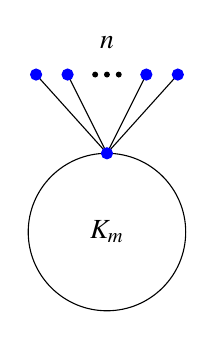
\begin{tikzpicture}[rotate=180] 
   
   \coordinate (c1) at ($(7,0) + (180:1)$);
   \coordinate (c2) at ($(7,0) + (225:1)$);
   \coordinate (c3) at ($(7,0) + (270:1)$);
   \coordinate (c4) at ($(7,0) + (315:1)$);
   \coordinate (c5) at ($(7,0) + (0:1)$);
   \coordinate (c6) at ($(7,0) + (45:1)$);
   \coordinate (c7) at ($(7,0) + (90:1)$);
   \coordinate (c8) at ($(7,0) + (135:1)$);
   
   \coordinate (e1) at ($(7,0) + (270:1) + (0.9,-1.0)$);
   \coordinate (e2) at ($(7,0) + (270:1) + (0.5,-1.0)$);
   \coordinate (e3) at ($(7,0) + (270:1) + (-0.5,-1.0)$);
   \coordinate (e4) at ($(7,0) + (270:1) + (-0.9,-1.0)$);
   
   \coordinate (b1) at ($(7,0) + (270:1) + (0.15,-1.0)$);
   \coordinate (b2) at ($(7,0) + (270:1) + (0,-1.0)$);
   \coordinate (b3) at ($(7,0) + (270:1) + (-0.15,-1.0)$);
   
   \coordinate (lb2) at ($(7,0) + (270:1) + (0,-1.4)$);   
      
  
%   \draw[draw=black] (c1) -- (c2);
%   \draw[draw=black] (c1) -- (c3);
%   \draw[draw=black] (c1) -- (c4);
%   \draw[draw=black] (c1) -- (c5);
%   \draw[draw=black] (c1) -- (c6);
%   \draw[draw=black] (c1) -- (c7);  
%   \draw[draw=black] (c1) -- (c8);
%
%   \draw[draw=black] (c2) -- (c3);
%   \draw[draw=black] (c2) -- (c4);
%   \draw[draw=black] (c2) -- (c5);
%   \draw[draw=black] (c2) -- (c6);
%   \draw[draw=black] (c2) -- (c7);  
%   \draw[draw=black] (c2) -- (c8); 
%
%   \draw[draw=black] (c3) -- (c4);
%   \draw[draw=black] (c3) -- (c5);
%   \draw[draw=black] (c3) -- (c6);
%  \draw[draw=black] (c3) -- (c7);  
%   \draw[draw=black] (c3) -- (c8); 
%
%   \draw[draw=black] (c4) -- (c5);
%   \draw[draw=black] (c4) -- (c6);
%   \draw[draw=black] (c4) -- (c7);  
%   \draw[draw=black] (c4) -- (c8);
%   
%   \draw[draw=black] (c5) -- (c6);
%   \draw[draw=black] (c5) -- (c7);  
%   \draw[draw=black] (c5) -- (c8); 
%
%   \draw[draw=black] (c6) -- (c7);  
%   \draw[draw=black] (c6) -- (c8);  
% 
%   \draw[draw=black] (c7) -- (c8);
    
   \draw[draw=black] (c3) -- (e1);   
   \draw[draw=black] (c3) -- (e2);   
   \draw[draw=black] (c3) -- (e3);   
   \draw[draw=black] (c3) -- (e4);   
   
   %\draw (7,0) circle [radius=1];   
   \draw[black] (7,0) node[circle,minimum size=2cm,draw] (v1) {$K_m$};

   %\filldraw[fill=blue,draw=blue] (c1) circle [radius=0.07];
   %\filldraw[fill=blue,draw=blue] (c2) circle [radius=0.07];
   \filldraw[fill=blue,draw=blue] (c3) circle [radius=0.07];
   %\filldraw[fill=blue,draw=blue] (c4) circle [radius=0.07];
   %\filldraw[fill=blue,draw=blue] (c5) circle [radius=0.07];
   %\filldraw[fill=blue,draw=blue] (c6) circle [radius=0.07];
   %\filldraw[fill=blue,draw=blue] (c7) circle [radius=0.07];
   %\filldraw[fill=blue,draw=blue] (c8) circle [radius=0.07];

   \filldraw[fill=blue,draw=blue] (e1) circle [radius=0.07];
   \filldraw[fill=blue,draw=blue] (e2) circle [radius=0.07];
   \filldraw[fill=blue,draw=blue] (e3) circle [radius=0.07];
   \filldraw[fill=blue,draw=blue] (e4) circle [radius=0.07];
   
   \filldraw[black] (lb2) node {$n$};   
   
   \filldraw[fill=black] (b1) circle [radius=0.03];
   \filldraw[fill=black] (b2) circle [radius=0.03];   
   \filldraw[fill=black] (b3) circle [radius=0.03];
      
\end{tikzpicture}}
}
\endgroup
\end{center}
\caption{The pineapple graph, $PA(m,n)$.}
   \label{fig-pn4}
\end{figure}


\begin{lemma}\label{spectral radius and average degree}
We have $\lambda_1(H) = \frac{n}{2} + c_1\sqrt{n}$ and $\frac{2e(H)}{n} = \frac{n}{4} + c_2\sqrt{n}$, where $|c_1|, |c_2|<1$.
\end{lemma}

\begin{proof}
By eigenvalue interlacing, $\mathrm{PA}(p,q)$ has spectral radius at least $p-1$. A calculation shows 
that for $H = \mathrm{PA}\left( \left\lceil \frac{n}{2}\right\rceil +1, \left\lfloor\frac{n}{2}\right\rfloor-1\right)$, we have 
\[
\lambda_1(H) - \frac{2e(H)}{n} \geq \frac{n}{4} - \frac{3}{2}.
\]
On the other hand, the eigenvector equation gives 
\[
\lambda_1^2 = \sum_{y\sim x} \lambda_1 y = \sum_{y\sim x}\sum_{z\sim y} z \leq \sum_{y\sim x}d_y \leq 2e(G) - (n-1),
\]
where the last inequality follows because $G$ is connected. This gives
\begin{equation}\label{lower bound on average degree}
d \geq \frac{\lambda_1^2}{n} + 1 - \frac{1}{n}.
\end{equation}
Setting $\lambda_1 = pn$ and applying \eqref{lower bound on average degree}, we have $\lambda_1 - d \leq pn - p^2n -1 + \frac{1}{n}$. The right hand side of the inequality is maximized at $p=1/2$, giving 
\begin{equation}\label{tight bound on irregularity}
\frac{n}{4} - \frac{3}{2} \leq \lambda_1 - d \leq \frac{n}{4} - 1 + \frac{1}{n}.
\end{equation}

Next setting $\lambda_1 = \frac{n}{2} + c_1 \sqrt{n}$, \eqref{lower bound on average degree} gives
\[
d \geq \frac{n}{4} + c_1\sqrt{n} + c_1^2 + 1 - \frac{1}{n},
\]
whereas \eqref{tight bound on irregularity} gives
\begin{equation}\label{d bar bound}
d \leq \lambda_1 - \frac{n}{4} + \frac{3}{2}  = \frac{n}{4} + c_1\sqrt{n}  + \frac{3}{2}.
\end{equation}
Together, these imply $|c_1| <1$ and prove both statements for $n$ large enough.
\end{proof}

\begin{lemma}\label{error in x neighborhood small}
There exists a constant $c_3$ not depending on $n$ such that 
\[
0 \leq \frac{1}{|N(x)|} \sum_{y\sim x} d_y - \lambda_1 y \leq c_3\sqrt{n}.
\]
\end{lemma}

\begin{proof}
By the eigenvector equation
\[
\sum_{y\sim x} \lambda_1 y = \lambda_1^2 = \sum_{y\sim x}\sum_{z\sim y} z \leq \sum_{y\sim x} d_y \leq dn - (n-1).
\]
Rearranging and applying Lemma \ref{spectral radius and average degree}, we have
\[
0\leq \sum_{y\sim x} \left( d_y - \lambda_1 y \right) = O\left(n^{3/2}\right).
\]
By the eigenvector equation again, and because the first eigenvector is normalized with $x=1$, we have
\[
\lambda_1 = \sum_{y\sim x} y \leq d_x,
\]
giving $d_x = \Omega(n)$. Combining, we have 
\[
\frac{1}{|N(x)|} \sum_{y\sim x} \left( d_y - \lambda_1 y \right) = O\left(\sqrt{n}\right),
\]
where the implied constant is independent of $n$.
\end{proof}

Now we fix a constant $\epsilon > 0$, whose exact value will be 
chosen later.  The next lemma implies that close to half of the vertices of
$G$ have eigenvector entry close to $1$ for $n$ sufficiently large, 
depending on the chosen $\epsilon$.  We follow that with a proposition
which outlines the approximate structure of $G$, and then finally use
variational arguments to deduce that $G$ is exactly a pineapple graph.


\begin{lemma}\label{u good}
 There exists a vertex $u\not=x$ with $u > 1- 2 \epsilon$ and $d_u - \lambda_1 u = O(\sqrt{n})$.  Moreover $d_u \geq \left( 1/2 - 2\epsilon \right)n$.
\end{lemma}


%\begin{lemma}\label{y good}
%Let $\epsilon >0$. There exists a $y\in N(x)$ such that $y> \frac{1}{2} - \epsilon$ and $d_y - \lambda_1 y < c_\epsilon \sqrt{n}$ where $c_\epsilon$ is a constant depending only on $\epsilon$.
%\end{lemma}

\begin{proof}
We proceed by first showing a weaker result: that there is a vertex $y$ with
$y> \frac{1}{2} - \epsilon$ and $d_y - \lambda_1 y = O(\sqrt{n})$, and 
additionally that $y \in N(x)$.  We will use then use this to bootstrap
the required result.


Let $A: = \{z\sim x: z> \frac{1}{2} - \epsilon\}$. By Lemma \ref{spectral radius and average degree},
\[
\lambda_1 = \frac{n}{2} + c_1\sqrt{n}
\]
where $|c_1| <1$. Since $0< z\leq 1$ for all $z\sim x$, we have that $|A| \geq \delta_\epsilon n$ where $\delta_\epsilon$ is a positive constant that depends only on $\epsilon$. Let $B = \{z\sim x: d_z - \lambda_1 z >  K\sqrt{n}\}$, where $K$ is a fixed constant whose exact value will be chosen later. Now
\[
\frac{1}{|N(x)|} \sum_{y\sim x} \left( d_y -\lambda_1 y \right) \geq \frac{1}{|N(x)|} \sum_{z\in B} \left( d_z - \lambda_1 z \right) \geq \frac{1}{n} |B| K\sqrt{n}.
\]
By Lemma \ref{error in x neighborhood small}, $|B| \leq \frac{c_3}{K} n$. Therefore, for $K$ large enough depending only on $\epsilon$, we have $\left|A\cap B^c\right| > 0$.  This proves the existence of the vertex $y$,
with the properties claimed at the beginning of the proof.


Next, we show that there exists a set $U\subset N(y)$ such that 
$|U| \geq \left(\frac{1}{4} - 2\epsilon \right)n$ and 
$u \geq 1-2\epsilon$ for all $u\in U$.  By Lemma \ref{spectral radius and average degree},
\[
\left(\frac{n}{2} + c_1\sqrt{n}\right)\left(\frac{1}{2} - \epsilon\right) \leq \lambda_1 y \leq d_y,
\]
where $|c_1| < 1$. So $d_y \geq \left(\frac{1}{4} - \epsilon \right) n$ for $n$ large enough. Now let $C = \{z\sim y: z < 1-2\epsilon \}$. Then
\[
K \sqrt{n} \geq d_y - \lambda_1 y = \sum_{z\sim y} \left( 1 - z \right) \geq \sum_{z\in C} \left( 1-z \right) \geq 2|C| \epsilon.
\]
Therefore
\[
|N(y) \setminus C| \geq \left(\frac{1}{4} - \epsilon\right)n  - \frac{K \sqrt{n}}{2\epsilon}.
\]
Setting $U = N(y) \setminus C$, we have $|U| > \left(\frac{1}{4} - 2\epsilon\right)n$ for $n$ large enough. 


Set $D = U \cap N(x)$.  We will first find a lower bound on $|D|$.  We have
 \begin{equation*}
  \lambda_1^2 \leq \sum_{y \sim x} d_y \leq 2m - \sum_{y \not \in N(x)} d_y
 \end{equation*}
Rearranging this we get 
 \[ d - \frac{\lambda_1^2}{n} \geq \frac{1}{n} \sum_{y \not \in N(x)} d_y\]
Now applying the bound on $d$ from equation~\ref{d bar bound} and expression for $\lambda_1$ in Lemma~\ref{spectral radius and average degree} yields
 \[ \left( \frac{n}{4} + c_1 \sqrt{n} + \frac{3}{2}\right) - \frac{\left(\frac{n}{2} + c_1 \sqrt{n}\right)^2}{n} \geq \frac{1}{n} \sum_{y \not \in N(x)} d_y \]
which implies that
 \[ \frac{3}{2} n \geq \left( \frac{3}{2} - c_1^2 \right) n \geq \sum_{y \not \in N(x)} d_y \geq \sum_{y \in U\setminus N(x)} d_y \geq |U\setminus N(x)| (1-2\epsilon) \lambda_1 .\]
So 
 \[ |U \setminus N(x)| \leq \frac{3}{2(1-2\epsilon)} \frac{n}{\lambda_1} = \frac{3}{2(1-2\epsilon)} \frac{1}{1/2 + c_1 n^{-1/2}} .\]
In particular, $|D| \geq (\frac{1}{4} - c'_\epsilon) n$.

Now by the same argument used at the start of the proof to show the existence
of the vertex $y$, we have some vertex $u \in D$
with $d_u - \lambda_1 u = O(\sqrt{n}$).   Finally 
\[d_u \geq u \lambda_1 \geq (1 - 2 \epsilon) (n/2 + c_1\sqrt{n}) \geq \left( 1/2 - 2\epsilon \right)n .  \]

\end{proof}

\subsection{Alteration Step}

\begin{lemma}\label{modifying conditions}
 Let $x,y$ be two vertices in $G$.  If
 $xy > 1/2 +n^{-1/2} + 5n^{-1}$, then $x$ and $y$ are adjacent.  On the
 other hand, if $xy < 1/2 - 3\epsilon$ then $x$ and $y$ are not adjacent.
\end{lemma}
\begin{proof}
We begin by bounding the dot product of the leading eigenvector $\textbf{v}$
with itself, we will show that
\begin{equation}\label{vvt bound}
\frac{n}{2} + \sqrt{n} + 5 \geq \textbf{v}^t\textbf{v} > \frac{n}{2} - 2 \epsilon n  - O(\sqrt{n})
\end{equation}


\noindent First, we show the lower bound.  With $u$ from the previous lemma, by Cauchy--Schwarz we have
\[  \textbf{v}^t\textbf{v} \geq \sum_{z \sim u} z^2 \geq \frac{1}{d_u}\left( \sum_{z \sim u} z \right)^2 = \frac{(\lambda_1 u)^2}{d_u} \]
By Lemma~\ref{u good}, we then have
 \[\textbf{v}^t\textbf{v} \geq \frac{(d_u - O(\sqrt{n}))^2}{d_u} \geq d_u - O(\sqrt{n}) > \frac{n}{2} - 2 \epsilon n  - O(\sqrt{n}) .\]
For the upper bound of inequality~\eqref{vvt bound}, first set $E = \left( N(x) \cup \{x\}\right)^C$.  Then
 \[ \textbf{v}^t\textbf{v} = \sum_{z \in V(G)} z^2 \leq \sum_{z \in V(G)} z \leq 1 + \sum_{z \in N(x)} z + \sum_{z \in E} z \leq 1 + \lambda_1 + \frac{1}{\lambda_1} \sum_{z \in E} d_z .\]
From the proof of Lemma~\ref{u good} we have the bound
 \[ \sum_{ z \in E} d_z \leq \frac{3}{2} n .\]
Hence
 \[ \textbf{v}^t \textbf{v}  \leq 1 + \frac{n}{2} + c_1 \sqrt{n} + \frac{3}{2} \cdot \frac{1}{1/2 + c_1 n^{-1/2}} \leq \frac{n}{2} + \sqrt{n} + 5 .\]
This completes the proof of inequality~\eqref{vvt bound}.


 Let $\lambda_1^+$ be the leading eigenvalue of the graph formed by adding the 
 edge $\{x,y\}$ to $G$.  Then by \eqref{rayleigh quotient} we have
  \[ \lambda_1^+ - \lambda_1 \geq \frac{\textbf{v}^t (A^+-A) \textbf{v}}{\textbf{v}^t \textbf{v}} \geq \frac{2xy}{\textbf{v}^t \textbf{v}} \geq \frac{2xy}{n/2 + \sqrt{n} + 5}  = \frac{2xy}{n(1/2+n^{-1/2} + 5 n^{-1})}.\]
If $xy > 1/2+n^{-1/2} + 5n^{-1}$, then
\[ (\lambda_1^+ - d^+) - (\lambda - d) > \frac{2}{n} - \frac{2}{n} \geq 0\]
Hence $\left\{x,y\right\}$ must already have been an edge, otherwise this
would contradict the maximality of $G$.

Similarly if $\lambda_1^-$ is the leading eigenvalue of the graph obtained
from $G$ by deleting the edge $\{x,y\}$, then  
  \[ \lambda_1 - \lambda_1^- \leq \frac{\textbf{v}^t (A-A^-) \textbf{v}}{\textbf{v}^t \textbf{v}} \leq \frac{2xy}{n/2 - 2\epsilon n - O(\sqrt{n})} \leq \frac{2xy}{(1/2 - 3 \epsilon)n}\]
when $n$ is large enough.  Now if
$xy < 1/2 - 3\epsilon$, then 
 \[ (\lambda_1 - d) - (\lambda_1^- - d^-) < 0 .\] %XXX: this doesn't typeset well

\end{proof}

%%%%%%%%%%%%%%%%%%picture%%%%%%%%%%%%%

\begin{figure}[]
\begin{center}
\begingroup

\setlength{\unitlength}{.01cm}
{
\setlength{\fboxsep}{10pt}
\framebox[1.5\width]{
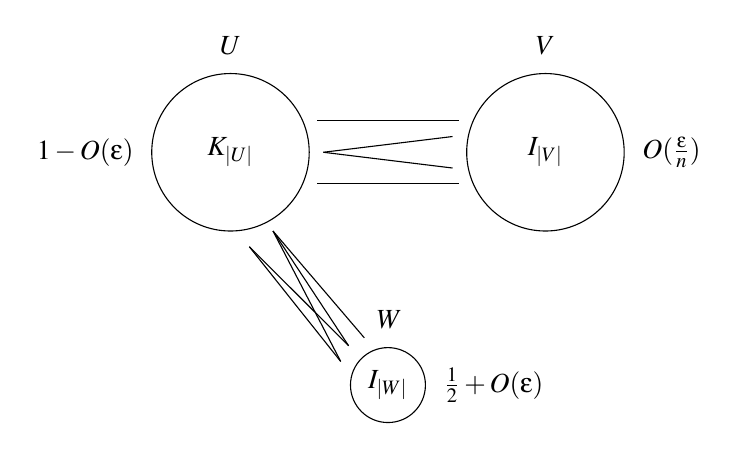
\begin{tikzpicture}
\filldraw[black] (0.553380,1.150606) node[label={[label distance=0.1cm]180:$1 - O(\epsilon)$},label={[label distance=0.1cm]$U$},circle,minimum size=2cm,draw] (v0) {$K_{|U|}$};

\filldraw[black] (4.553380,1.150606) node[label={[label distance=0.1cm]0:$O(\frac{\epsilon}{n})$},label={[label distance=0.1cm]$V$},circle,minimum size=2cm,draw] (v1) {$I_{|V|}$};

\filldraw[black] (2.553380,-1.80606) node[label={[label distance=0.1cm]0:$\frac{1}{2}+O(\epsilon)$},label={[label distance=0.1cm]88:$W$},circle,minimum size=0.8cm,draw] (v1) {$I_{|W|}$};

\coordinate (UC) at (0.553380,1.150606);
\coordinate (VC) at (4.553380,1.150606);
\coordinate (WC) at (2.553380,-1.80606);

\coordinate (Ul1) at ($(UC) + (1.1,-0.4)$);
\coordinate (Ul2) at ($(UC) + (1.18,-0)$);
\coordinate (Ul3) at ($(UC) + (1.1,0.4)$);

\coordinate (Ub2) at ($(UC) + (0.24,-1.2)$);
\coordinate (Ub3) at ($(UC) + (0.54,-1.0)$);


\coordinate (Vl1) at ($(VC) + (-1.1,-0.4)$);
\coordinate (Vl2a) at ($(VC) + (-1.18,-0.2)$);
\coordinate (Vl2b) at ($(VC) + (-1.18,0.2)$);
\coordinate (Vl3) at ($(VC) + (-1.1,0.4)$);

\coordinate (Wt1) at ($(WC) + (-0.5,0.5)$);
\coordinate (Wt2) at ($(WC) + (-0.3,0.6)$);
\coordinate (Wt3) at ($(WC) + (-0.6,0.3)$);


\draw (Ul1) -- (Vl1);
\draw (Ul2) -- (Vl2a);
\draw (Ul2) -- (Vl2b);
\draw (Ul3) -- (Vl3);

\draw (Ub3) -- (Wt1);
\draw (Ub3) -- (Wt2);
\draw (Ub3) -- (Wt3);

\draw (Ub2) -- (Wt3);
\draw (Ub2) -- (Wt1);

%\draw[black] (v0) -- (v1);

\end{tikzpicture}}
}
\endgroup
\end{center}
\caption{Structure of $G$ in Proposition \ref{almost pineapple structure}.  The number beside
each set indicates the values of eigenvector entries in the set. 
$U$ is a clique, $V$, $W$ are independent sets.  Vertices in $V$ are adjacent
to one vertex in $U$, and vertices in $W$ are adjacent to multiple vertices in $U$.
   \label{pineapple structure picture}}
\end{figure}

%%%%%%%%%%%%%%%%%%%%%%%%

\begin{proposition}\label{almost pineapple structure}
For $n$ sufficiently large, we can partition the vertices of $G$ into three 
sets $U, V, W$ (see Figure \ref{pineapple structure picture}) where 
\begin{itemize}
 \item[(i)] vertices in $V$ have eigenvector entry smaller than $(2+\epsilon) / n$ and have degree one, 
 \item[(ii)] vertices in $U$ induce a clique, 
 all have eigenvector entry larger than $1 - 20\epsilon$, and $(1/2 - 3\epsilon) n \leq |U| \leq (1/2 + \epsilon)n$,

 \item[(iii)] vertices in $W$ have eigenvector entry in the range $\left[1/2 - 4\epsilon,  1/2 + 21 \epsilon \right]$ and are adjacent only to vertices in $U$.  
\end{itemize}
\end{proposition}

\begin{proof}
  By Lemma~\ref{modifying conditions}, any two vertices in $G$ with eigenvector entry $1$ are adjacent.  Moreover, it is easy to see that
  every vertex in $G$ is incident to at least one vertex with eigenvector entry $1$:  if not, for each vertex not incident to a vertex
  with eigenvector entry $1$, delete one of its edges and add a new edge from that vertex to a vertex with eigenvector entry $1$ (such as
  the vertex $x$).  The resulting graph is connected, will have the same number of edges as the original graph, and will have strictly larger $\lambda_1$
  (this can be seen by considering the Rayleigh quotient, as in the proof of Lemma~\ref{modifying conditions}).
  So by maximality of $G$, there are no such vertices.  This implies that the set of edges that are incident
  to a vertex with eigenvector entry $1$ spans the vertex set of $G$. 
  In particular, if we remove any edge that is not incident to a vertex with eigenvector entry $1$, we do not disconnect the graph.  We will use this fact repeatedly in this proof.

 
  
\begin{itemize}
\item[(i)] Let $V$ consist of all vertices in $G$ with eigenvector entry 
less than $1/2 - 4 \epsilon$.  By Lemma~\ref{modifying conditions}, removing 
any edge incident to a vertex in $V$ strictly increases $\lambda_1 - d$, so each vertex in $V$ has degree one.  By the eigenvector equation,
the eigenvector entry of any such vertex is at most $1/\lambda_1 < (2+\epsilon) / n $, when $n$ is large enough.
\item[(ii)] From Lemma~\ref{u good}, we have a vertex $u$ such that $d_u - \lambda_1 u = O(\sqrt{n})$.  Let $X$ be the set of neighbors $z$ of $u$ such that $z < 9/10$.  Then we have
 \[ (1 - 9/10)|X| \leq \sum_{y \sim u} 1 - y = d_u - \lambda_1 u = O(\sqrt{n}). \]
Hence $|X| = O(\sqrt{n})$.  Let $U$ be all vertices in $G$ with eigenvector entry at least $9/10$.  So, by Lemma~\ref{u good}
 \[ |U| \geq d_u - |X| \geq n/2 - 2 \epsilon n - O(\sqrt{n})\]
For $n$ large enough, we have $|U| \geq (1/2 - 3\epsilon) n$. For sufficiently large $n$, by Lemma~\ref{modifying conditions} these vertices are all adjacent to each other.  For the upper bound on $|U|$ we use the expression for $e(G)$ in Lemma~\ref{spectral radius and average degree}
\[ |U| (|U| - 1) \leq 2e(G) \leq  \frac{n^2}{4} + c_2n\sqrt{n}\]
which implies $|U| \leq (1/2+\epsilon) n$ for large enough $n$.

Now take any vertex $y \in U$.  If $x$ is a vertex with largest eigenvector entry, then 
\begin{equation}\label{y_bound}
 \lambda_1 - \lambda_1 y \leq \sum_{z \in N(x) \setminus N(y)} z \leq y + \sum_{z \in U^C} z 
\end{equation}
We have
 \begin{eqnarray*}
  \lambda_1 \sum_{z \in U^C} z \leq \sum_{z \in U^C} d_z &\leq& 2e(G) - 2|E(U,U)|\\
   &\leq& \frac{n^2}{4} + c_2 n \sqrt{n} - (1/2 - 3\epsilon)(1/2 - 3 \epsilon - 1/n) n^2 \\
   &\leq & 4 \epsilon n^2
 \end{eqnarray*}
for $n$ sufficiently large, where we are using the expression for $e(G)$ given by Lemma~\ref{spectral radius and average degree}.
In particular,
 \[ \sum_{z \in U^C} z \leq 9 \epsilon n \] 
Finally, by equation~\ref{y_bound} we have 
 \[ y \geq 1 - \frac{1}{\lambda_1} \sum_{z \in U^C} z -\frac{y}{\lambda_1} \geq (1 - 20 \epsilon) .\]
 
\item[(iii)] Let $W$ consist of all remaining vertices of $G$.  If a vertex 
has eigenvector entry smaller than $1/2 - 4\epsilon$ then it is in $V$ by
construction.  If a vertex $z \in W$ has eigenvector entry larger than $1/2 + 21\epsilon$
then we have
 \[ (1/2 + 21 \epsilon) (1 - 20 \epsilon) > 1/2 + \epsilon \]
if $\epsilon < 1/50$, say.   So for sufficiently large $n$, by Lemma~\ref{modifying conditions} we 
have that $z$ is adjacent to every vertex in $U$.  But by the proof of part (ii), this implies that $z > 1 - 20\epsilon$, which contradicts $z \in W$.

For $z \in W$ and any vertex $y \in U^C$, then 
 $yz \leq (1/2 + 21 \epsilon)(1/2 + 21\epsilon) < 1/4 + 22 \epsilon$
and so by Lemma~\ref{modifying conditions} there is no edge between $y$ and 
$z$ in the maximal graph $G$.
\end{itemize}
\end{proof}

\subsection{The Pineapple Graph is Extremal}

\begin{theorem}
For sufficiently large $n$, $G$ is a pineapple graph.
\end{theorem}
\begin{proof}
Take $U,V,W$ as in the previous lemma.  We begin by showing that the set $W$ must be empty.  Assume to the contrary, and let $z$ be in $W$, and furthermore
let $G^+$ be the graph obtained by adding edges from $z$ to every vertex in $U$.
We will show that $\lambda_1(G^+) - d(G^+) > \lambda_1(G) - d(G)$, which contradicts the maximality of $G$.

Since the vertex $z$ is adjacent only to vertices in $U$, and the
fact that vertices in $U$ have eigenvector entry between $1-20\epsilon$ and $1$,
the eigenvector equation yields
 \[\lambda_1 (1/2 - 4 \epsilon) \leq \lambda_1 z \leq d_z(G) \leq \frac{\lambda_1 z}{1 - 20 \epsilon} = (1/2 + O(\epsilon))\lambda_1\]

\noindent Using the expression for $\lambda_1$ in Lemma~\ref{spectral radius and average degree}, for large enough $n$ we have
 \[ \left(1-\epsilon\right)\frac{n}{4} \leq d_z(G) \leq \left(1+\epsilon\right) \frac{n}{4}\]
So we can bound the change in the average degrees
 \[ d(G^+) - d(G) \leq \frac{2(|U| - (1-\epsilon)n/4)}{n}< 1/2 + 3\epsilon\]
Next we find a lower bound on $\lambda_1(G^+) - \lambda_1(G)$.  Recall that $\textbf{v}$
is the leading eigenvector of $A(G)$, normalized so that $||\textbf{v}||_\infty = 1$.  Let $\textbf{w}$ be the vector that is equal to $\textbf{v}$ on all 
vertices except $z$, and equal to $1$ for $z$.  Then, 
 \[ \lambda_1(G^+) \geq \frac{\textbf{w}^tA^+\textbf{w}}{\textbf{w}^t\textbf{w}}\] 
We first find a lower bound for the numerator (with abuse of big-O notation with inequalities)
\begin{eqnarray*} 
\textbf{w}^tA^+\textbf{w} & \geq & \textbf{w}^tA\textbf{w} + 2(|U| - d_z(G))(1-O(\epsilon)) \geq \textbf{w}^tA\textbf{w} + (1/2-O(\epsilon))n \\
& \geq &  \textbf{v}^tA\textbf{v} + 2d_z(G) \left(1-z\right)(1-20\epsilon) + (1/2-O(\epsilon))n \\
%& \geq &  \textbf{v}^tA\textbf{v} + 2d_z(G) \left(1/2 - 21\epsilon\right)(1-20\epsilon) + (1/2-O(\epsilon))n \\
& \geq &  \textbf{v}^tA\textbf{v} + 2d_z(G) \left(1/2 - 31\epsilon\right) + (1/2-O(\epsilon))n \\
%& \geq & \textbf{v}^tA\textbf{v} + 2(1-\epsilon)(n/4) \left(1/2 - 31\epsilon\right) + (1/2-O(\epsilon))n \\
%& \geq & \textbf{v}^tA\textbf{v} + (n/4) \left(1 - 63\epsilon\right) + (1/2-O(\epsilon))n\\
& \geq &  \textbf{v}^tA\textbf{v} + (3/4-O(\epsilon))n
\end{eqnarray*}
Similarly, we find an upper bound for the denominator
\begin{eqnarray*}
\textbf{w}^t \textbf{w} &=& \textbf{v}^t\textbf{v} + 1 - z^2 \\
&\leq& \textbf{v}^t\textbf{v} + 1 - (1/2 - 4\epsilon)^2 \\
&\leq& \textbf{v}^t\textbf{v} + 3/4 + 4\epsilon
\end{eqnarray*}
Combining these, and using the bound on $\textbf{v}^t\textbf{v}$ from
the proof of Lemma~\ref{modifying conditions}, we get
\begin{eqnarray*}
 \lambda_1(G^+) - \lambda_1(G) &\geq& \frac{\textbf{w}^tA^+\textbf{w}}{\textbf{w}^t\textbf{w}} - \frac{\textbf{v}^tA\textbf{v}}{\textbf{v}^t\textbf{v}}\\
% & \geq & \frac{\textbf{v}^tA\textbf{v} + (1-37\epsilon)3n/4}{\textbf{v}^t\textbf{v} + 3/4 + 4\epsilon} -  \frac{\textbf{v}^tA\textbf{v}}{\textbf{v}^t\textbf{v}}\\
 &\geq& \frac{\textbf{v}^t\textbf{v}(3/4-O(\epsilon))n - \textbf{v}^tA\textbf{v} (3/4 + 4\epsilon)}{\textbf{v}^t\textbf{v} (\textbf{v}^t\textbf{v} + 3/4 + 4\epsilon)}\\
 &\geq & \frac{(3/4-O(\epsilon))n - (3/4 + 4\epsilon)\lambda_1(G)}{\textbf{v}^t\textbf{v} + 3/4 + 4\epsilon} \\ 
 &= &  3/4 + O(\epsilon)
\end{eqnarray*}
Hence $\lambda_1(G^+) - \lambda_1(G) > d(G^+) - d(G)$, and by maximality of $G$ we conclude that $W = \emptyset$.

At this point we know that $G$ consists of a clique together with a set of pendant vertices $V$.  All that remains is to show that all of the pendant vertices  are incident to the same vertex in the clique.  Let $V = \left\{v_1, v_2, \cdots, v_k\right\}$, and let $u_i$ be the unique vertex in $U$ that $v_i$ is adjacent to.  Let $G^+$ be the graph obtained from $G$ by deleting the edges $\left\{v_i,u_i\right\}$ and adding the edges $\left\{v_i,x\right\}$, where $x$ is a vertex with eigenvector entry $1$.  Now, $d(G^+) = d(G)$, and 
\[ \lambda_1(G^+) -\lambda_1(G) \geq \frac{\textbf{v}^t A^+ \textbf{v}}{\textbf{v}^t\textbf{v}} - \frac{\textbf{v}^t A \textbf{v}}{\textbf{v}^t\textbf{v}}\]
with equality if and only if $\textbf{v}$ is a leading eigenvector for $A^+$.  We have
\[\frac{\textbf{v}^t A^+ \textbf{v}}{\textbf{v}^t\textbf{v}} - \frac{\textbf{v}^t A \textbf{v}}{\textbf{v}^t\textbf{v}} = \frac{1}{\textbf{v}^t\textbf{v}}\left( \sum_{i=1}^k 1 - u_i \right) \geq 0\]
with equality if and only if $u_i = 1$ for all $1 \leq i \leq k$.  By maximality of $G$, we have equality in both of the above inequalities, and so $\textbf{v}$ is a leading eigenvector for $G^+$, and every vertex in $U$ incident to a vertex in $V$ has eigenvector entry 1.  $G^+$ is a pineapple graph, and it is easy to see that there is a single vertex in a pineapple graph with maximum eigenvector entry.  It follows that the vertices in $V$ are all adjacent to the same vertex in $U$, and hence $G$ is a pineapple graph.

\end{proof}


This chapter is based on the papers ``Three conjectures in extremal spectral graph theory'',
 \cite{TaitTobin2017}, to appear in \textit{Journal of Combinatorial Theory, Series B},
 and ``Characterizing graphs of maximum principal ratio'', submitted to
 \textit{Electronic Journal of Linear Algebra} \cite{TaitTobin2015},
both written jointly with Michael Tait.  The dissertation
author was the primary investigator and author of the paper.


%
% Of course, if you prefer, you can just start with
%   \chapter{My First Chapter Name}
% and start typing away.  

\chapter{Introduction}

\section{Preliminaries}

\section{Spectral Graph Theory}

\subsection{Fundamentals of Linear Algebra}

\subsection{Matrices Associated to Graphs}

\subsection{Graph Coverings and Projections}

\section{Overview of Results}

%\section{A section}
Lorem ipsum dolor sit amet, consectetuer adipiscing elit. Nulla odio
sem, bibendum ut, aliquam ac, facilisis id, tellus. Nam posuere pede
sit amet ipsum. Etiam dolor. In sodales eros quis pede.  Quisque sed
nulla et ligula vulputate lacinia. In venenatis, ligula id semper
feugiat, ligula odio adipiscing libero, eget mollis nunc erat id orci.
Nullam ante dolor, rutrum eget, vestibulum euismod, pulvinar at, nibh.
In sapien. Quisque ut arcu. Suspendisse potenti. Cras consequat cursus
nulla.

%\subsection{A Figure Example}
\label{ssec:figure_example}

%This subsection shows a sample figure.

%\begin{figure}[h] 
%  \centering
%  \includegraphics[width=0.5\textwidth]{sandiego}
%  \caption[Short figure caption (must be \protect{$< 4$} lines in the list of figures)]{A picture of San Diego.  Note that figures must be on their own line (no neighboring text) and captions must be single-sp%aced and appear \protect\textit{below} the figure.  Captions can be as long as you want, but if they are longer than 4 lines in the list of figures, you must provide a short figure caption.\index{SanDiego}} 
%  \label{fig:sandiego}
%\end{figure}

%\subsection{A Table Example}

While in Section \ref{ssec:figure_example} Figure \ref{fig:sandiego} we had a majestic figure, here we provide a crazy table example.


%%%% TABLE 1 %%%%
\vspace{0.25in}
\begin{table}[!ht]
\caption[Short figure caption (must be \protect{$< 4$} lines in the list of tables)]{A table of when I get hungry.  Note that tables must be on their own line (no neighboring text) and captions must be single-spaced and appear \protect\textit{above} the table.  Captions can be as long as you want, but if they are longer than 4 lines in the list of figures, you must provide a short figure caption.}

\vspace{-0.25in}
\begin{center}
\begin{tabular}{|p{1in}|p{2in}|p{3in}|}

\hline
Time of day & Hunger Level & Preferred Food \\

\hline
8am & high & IHOP (French Toast) \\

\hline
noon & medium & Croutons (Tomato Basil Soup \& Granny Smith Chicken Salad) \\

\hline
5pm & high & Bombay Coast (Saag Paneer) or Hi Thai (Pad See Ew) \\

\hline
8pm & medium & Yogurt World (froyo!) \\

\hline
\end{tabular}
\end{center}
\label{tab:analysis3}
\end{table}



\chapter{Measures of Graph Irregularity}
\section{Introduction}

A \textit{measure of graph irregularity} is a  statistics that quantifies how far a graph is
from being regular.  The choice of the word ``measure'' is slightly unfortunate due to its
more common usage in mathematics, but this is the phrase that has been used repeatedly in the
literature, and so we adopt it here.  Many different such statistics have been proposed.
There is the \textit{irregularity of a graph} as defined by Albertson \cite{Albertson1997},
\[ \textrm{irr}(G) = \sum_{(u,v) \in E(G)} \left| d_u - d_v \right| .\]
A variant of this that depends only on the degree sequence of a graph,
the \textit{total irregularity}, was introduced by Abdo et. al. \cite{Abdo2014},
\[ \textrm{irr}_{\textrm{it}}(G) = \frac{1}{2} \sum_{u \in V(G)} \sum_{v \in V(G)} \left| d_u - d_v\right|\]
Another irregularity measure that does depends only on the degree sequence is given by the
variance of the degree sequence, studied by Bell \cite{Bell1992},
\[var(G) = \frac{1}{n} \sum_{v\in V(G)} \left| d_v - \bar{d} \right|^2 . \]
Collatz and Sinogowitz, in perhaps the first spectral graph theory paper, noted
that the difference between the largest adjacency eigenvalue and the average degree
can be seen as a measure of the irregularity of a connected graph \cite{CollatzSinogowitz1957}.
Finally, the \textit{principal ratio} of a connected graph was studied as a
measure of graph irregularity by Cioab\u{a} and Gregory \cite{CioabaGregory2007},
\[ \gamma(G) = \frac{\mathbf{x}_{\text{max}}}{\mathbf{x}_{\text{min}}},\]
where $\mathbf{x}$ is a positive eigenvector corresponding to the
largest eigenvalue of the adjacency matrix, and
$x_{\text{min}}$ and $x_{\text{max}}$ are the smallest and largest eigenvector
entries respectively.

In this section we determine the extremal graphs
with respect to the last two irregularity measures,
answering conjectures of Cioab\u{a} and Gregory \cite{CioabaGregory2007}
and Aouchiche et. al. \cite{AouchicheEtAl2008}.


Let $P_r \cdot K_s$ be the graph attained by identifying an end vertex
of a path on $r$ vertices to any vertex of a complete graph
on $s$ vertices.  This has been called a \textit{kite graph} or a
\textit{lollipop graph}.  Cioab\u{a} and Gregory \cite{CioabaGregory2007}
conjectured that the connected graph on $n$ vertices maximizing $\gamma$
is a kite graph.  Our first result proves this conjecture for $n$ large
enough.
\begin{theorem}\label{main_theorem}
  For sufficiently large $n$, the connected graph $G$ on $n$
  vertices with largest principal ratio is a kite graph.
\end{theorem}


A \textit{pineapple graph} is a clique with pendant edges added to a single vertex.
Aouchiche et al \cite{AouchicheEtAl2008} conjectured that the extremal connected
graph with respect to the invariant $\lambda_1 - d$ is a pineapple graph.  We
show this for sufficiently large $n$.
\begin{theorem}\label{main_theorem}
  For sufficiently large $n$, the connected graph $G$ on $n$
  that maximizes $\lambda_1 - d$ is a pineapple graph.
\end{theorem}



An analogous problem for directed graphs, finding graphs which maximize the
principal ratio for directed graphs, was answered by Aksoy et al \cite{AksoyEtAl2016}.
We note that Brightwell and Winkler \cite{BrightwellWinkler1990} showed that
a kite graph maximizes the expected hitting time of a random walk.
The extremal graphs for various of these irregularity measures have been
studied.  
The extremal graphs with respect to $\textrm{irr}(G)$
were characterized by Hansen and M\'elot \cite{HansenMelot2002},
and the extremal graphs with respect to the total irregularity
were studied by \cite{Abdo2014}.
Nikiforov \cite{Nikiforov2006} proved several inequalities comparing
$var(G)$, $\epsilon(G)$ and $s(G) := \sum_v |d(u) - \bar{d}|$.  
Bell showed that $\epsilon(G)$ and $var(G)$ are incomparable in general
\cite{Bell1992}.  Finally, additional bounds on $\gamma(G)$ have been given in
\cite{CioabaGregory2007, PapendieckRecht2000, Minc1970, Latham1995, Zhang2005}.


\section{Graphs of Maximal Principal Ratio}

\subsection{Structural Lemmas}
%XXX: move this stuff somewhere

Throughout this section $G$ will be a connected simple graph on $n$ vertices.
The eigenvectors and eigenvalues of $G$ are those of the adjacency
matrix $A$ of $G$.  The vector $v$ will be the eigenvector corresponding
to the largest eigenvalue $\lambda_1$,  and we take $v$ to be scaled
so that its largest entry is $1$.  Let $x_1$ and $x_k$
be the vertices with smallest and largest eigenvector entries respectively, and
if several such vertices exist then we pick any of them arbitrarily.
Let $x_1, x_2, \cdots, x_k$ be a shortest path between $x_1$ and
$x_k$.  Let $\gamma(G)$ be the principal ratio of $G$.  We will abuse
notation so that for any vertex $x$, the symbol $x$ will refer also to $v(x)$,
the value of the eigenvector entry of $x$.  For example, with this notation
the eigenvector equation becomes

 \[ \lambda v = \sum_{w \sim v} w. \]

%\noindent We will make use of the Rayleigh quotient characterization of the
%largest eigenvalue of a graph,

%\begin{equation}\label{rayleigh}
%  \lambda_1(G) = \max_{0 \neq v} \frac{v^T A(G) v}{v^t v} 
%\end{equation}


Recall that the vertices $v_1, v_2, \cdots, v_m$ are a 
\textit{pendant path} if the induced graph on these vertices
is a path and furthermore if, in $G$, $v_1$ has degree $1$ and
the vertices $v_2, \cdots, v_{m-1}$ have degree $2$
(note there is no requirement on the degree of $v_m$).

\begin{lemma}\label{path_bound}
  If $\lambda_1 \geq 2$ and $\sigma = (\lambda_1 + \sqrt{\lambda_1^2 - 4})/2$, then for
  $1 \leq j \leq k$,
   \[ \gamma(G) \leq \frac{\sigma^j - \sigma^{-j}}{\sigma - \sigma^{-1}} x_j^{-1}. \]
Moreover we have equality if the vertices $x_1, x_2, \cdots, x_{j}$ are a pendant path.
  
\end{lemma}
\begin{proof}
  We have the following system of inequalities
   \begin{eqnarray*}
     \lambda_1 x_1 & \geq & x_2 \\
     \lambda_1 x_2 & \geq & x_1 + x_3 \\
     \lambda_1 x_3 & \geq & x_2 + x_4 \\
     \vdots & & \vdots\\
     \lambda_1 x_{j-1} & \geq & x_j + x_{j-2}
   \end{eqnarray*}
 The first inequality implies that
  \[ x_1 \geq \frac{1}{\lambda_1} x_2\]
 Plugging this into the second equation and rearranging gives
  \[ x_2 \geq \frac{\lambda_1}{\lambda_1^2 - 1} x_3 \]
 Now assume that
  \[ x_i \geq \frac{u_{i-1}}{u_i} x_{i+1}. \]
 with $u_j$ positive for all $j<i$.  Then
  \[ \lambda_1 x_{i+1} \geq x_{i} + x_{i+2} \]
 implies that
  \[ x_{i+1} \geq \frac{u_i}{\lambda_1 u_i - u_{i-1}} x_{i+2}. \]
 where $\lambda_1 u_i - u_{i-1}$ must be positive because  $x_j$
 is positive for all $j$.
 Therefore the coefficients $u_i$ satisfy the recurrence
  \[ u_{i+1} = \lambda_1 u_i - u_{i-1}\]
 Solving this and using the initial conditions $u_0 = 1$,
 $u_1 = \lambda$ we get
  \[ u_i = \frac{\sigma^{i+1} - \sigma^{-i-1}}{\sigma - \sigma^{-1}} \]
 In particular, $u_i$ is always positive, a fact implicitly
 used above.  Finally this gives,
  \[ x_1 \geq \frac{u_0}{u_1} x_2 \geq \frac{u_0}{u_1} \cdot \frac{u_1}{u_2} x_3 \geq \cdots \geq \frac{x_j}{u_{j-1}} \]
 Hence
  \[ \gamma(G) = \frac{x_k}{x_1} = \frac{1}{x_1} \leq \frac{\sigma^j - \sigma^{-j}}{\sigma - \sigma^{-1}} x_j^{-1} \]
 If these vertices are a pendant path, then we have equality throughout.
\end{proof}

We will also use the following lemma which comes from the
paper of Cioab\u{a} and Gregory \cite{CioabaGregory2007}.

\begin{lemma}\label{kite_lambda}
  For $r \geq 2$ and $s \geq 3$,
   \[ s - 1 + \frac{1}{s(s-1)} < \lambda_1(P_r \cdot K_s) < s - 1 + \frac{1}{(s-1)^2} . \]
\end{lemma}

In the remainder of the section  we prove Theorem~\ref{main_theorem}.
We now give a sketch of the proof that is contained in Section~\ref{sec_proof}.

\begin{enumerate}
 \item We show that the vertices $x_1, x_2, \cdots, x_{k-2}$ are
   a pendant path and that $x_k$ is connected to all of the vertices
   in $G$ that are not on this path (lemma~\ref{connect_every}).
 \item Next we prove that the length of the path is approximately
   $n - n/\log(n)$ (lemma~\ref{s_range}).
 \item We show that $x_{k-2}$ has degree exactly $2$ (lemma~\ref{k_2_lemma}), which
   extends our pendant path to $x_1, x_2, \cdots, x_{k-1}$.
   To do this, we find conditions under which adding or deleting
   edges increases the principal ratio (lemma~\ref{change}).
 \item Next we show that $x_{k-1}$ also has degree exactly $2$ (lemma~\ref{k_1_lemma}).
   At this point we can deduce that our extremal graph is either
   a kite graph or a graph obtained from a kite graph
   by removing some edges from the clique.  We show that
   adding in any missing edges will increase the principal ratio,
   and hence the extremal graph is exactly a kite graph.
   
\end{enumerate}

\subsection{Proof of Main Theorem}\label{sec_proof}



Let $G$ be the graph with maximal principal ratio among all connected
graphs on $n$ vertices, and let $k$ be the number of vertices in a
shortest path between the vertices with smallest and largest eigenvalue
entries. As above, let $x_1,\cdots, x_k$ be the vertices of the shortest path, where $\gamma(G) = x_k / x_1$.  Let $C$ be the set of vertices not on this shortest
path, so $|C| = n-k$.  Note that there is no graph with $n-k=1$, as the endpoints of a path have the same principal eigenvector entry.  Also
$\lambda_1(G) \geq 2$, otherwise $P_{n-2} \cdot K_3$ would have larger
principal ratio.  Finally note that $k$ is strictly larger than $1$,
otherwise $x_k = x_1$ and $G$ would be regular.


\begin{lemma}\label{max_lambda}
  $\lambda_1(G) > n-k$.
\end{lemma}
\begin{proof}
  Let $H$ be the graph $P_k \cdot K_{n-k+1}$. It is straightforward to see that in $H$, the smallest entry of the principal eigenvector is the vertex of degree $1$ and the largest is the vertex of degree $n-k+1$. Also note that in $H$, the vertices on the path $P_k$ form a pendant path.
  By maximality we know that $\gamma(G) \geq \gamma(H)$.
  Combining this with lemma~\ref{path_bound}, we get
   \[ \frac{\sigma^k - \sigma^{-k}}{\sigma - \sigma^{-1}} \geq \gamma(G) \geq \gamma(H) =  \frac{\sigma_H^{k} - \sigma_H^{-k}}{\sigma_H - \sigma_H^{-1}} \]
  where $\sigma_H = \left(\lambda_1(H) + \sqrt{\lambda_1(H)^2 - 4}\right) /2$.

  \noindent Now the function
   \[ f(x) = \frac{x^k - x^{-k}}{x - x^{-1}}\]
  is increasing when $x \geq 1$.
  Hence we have
  $\sigma \geq \sigma_H$, and so
  $\lambda_1(G) \geq \lambda_1(H) > n-k$.
\end{proof}

\begin{lemma}\label{connect_every}
  $x_1, x_2, \cdots, x_{k-2}$ are a pendant path in $G$, and $x_k$
  is connected to every vertex in $G$ that is not on this
  path.
\end{lemma}
\begin{proof}
  By our choice of scaling, $x_k = 1$.  From lemma~\ref{max_lambda}
   \[ n-k < \lambda_1(G) = \sum_{y \sim  x_k} y \leq |N(x_k)|. \]
  Now $|N(x_k)|$ is an integer, so we have $|N(x_k)| \geq n-k+1$.
  Moreover because $x_1, x_2, \cdots, x_k$ is an induced path, we
  must have that $|N(x_k)| = n-k+1$ exactly, and hence the
  $N(x_k) = C \cup \{ x_{k-1} \}$.  It follows that $x_1, x_2, \cdots, x_{k-3}$
  have no neighbors off the path, as otherwise there would be a shorter
  path between $x_1$ and $x_k$.
\end{proof}

\begin{lemma}\label{s_range}
For the extremal graph $G$, we have $n-k = (1+o(1))\frac{n}{\log n}$.
\end{lemma}
\begin{proof}
Let $H$ be the graph $P_j \cdot K_{n-j+1}$ where $ j = \left\lfloor n - \frac{n}{\log n}\right\rfloor$, and let $G$ be the connected graph on $n$ vertices with maximum principal ratio. Let $x_1,\cdots, x_k$ be a shortest path from $x_1$ to $x_k$ where $\gamma(G) = \frac{x_k}{x_1}$. By lemma \ref{connect_every}, we have
\[
\lambda_1(G) \leq \Delta(G) \leq n-k+1.
\]
By the eigenvector equation, this gives that
\begin{equation}\label{gamma of G}
\gamma(G) \leq (n-k+1)^k
\end{equation}
Now, lemma \ref{path_bound} gives that
\[
\gamma(H)  = \frac{\sigma_H^j - \sigma_H^{-j}}{\sigma_H - \sigma_H^{-1}},
\]
where
\[
\sigma(H) = \frac{\lambda_1(H) + \sqrt{\lambda_1(H)^2 -4}}{2}.
\]

Now, $s-1 + \frac{1}{s(s-1)} < \lambda_1(P_r\cdot K_s) < s-1 + \frac{1}{(s-1)^2}$, so we may choose $n$ large enough that $\frac{n}{\log n} + 1 >\sigma_H - \sigma_H^{-1} > \frac{n}{\log n}$. By maximality of $\gamma(G)$, we have
\[
(n-k+1)^k \geq \gamma(G) \geq \gamma(H) \geq \left(\frac{n}{\log n}\right)^{n-\frac{n}{\log n} - 2}.
\]
Thus, $n- k = (1+o(1))\frac{n}{\log n}$.
\end{proof}

For the remainder of this section we will explore the structure of $G$ by
showing that if certain edges are missing, adding them would increase
the principal ratio, and so by maximality these edges must already be
present in $G$.  We have established that the vertices $x_1, x_2, \cdots, x_{k-2}$
are a pendant path, and so we have
\begin{equation}\label{pr_form}
 \gamma(G) = \frac{\sigma^{k-2} - \sigma^{-k+2}}{\sigma-\sigma^{-1}} \frac{1}{x_{k-2}}
\end{equation}
We will not add any edges that affect this path, and so the above equality will
remain true.   
The change in $\gamma$ is then completely determined by the change
in $\lambda_1$ and the change in $x_{k-2}$.  The next lemma gives conditions
on these two parameters under which $\gamma$ will increase or decrease.

\begin{lemma}\label{change}
Let $x_1, x_2, \cdots, x_{m-1}$ form a pendant path
  in $G$, where $n-m = (1+o(1)) n/\log(n)$.
  Let $G_+$ be a graph obtained from $G$ by adding some edges from $x_{m-1}$ to $V(G)\setminus \{x_1,\cdots, x_{m-1}\}$,
  where the addition of these edges does not affect which vertex
  has largest principal eigenvector entry.  Let
  $\lambda_1^+$ be the largest eigenvalue of $G_+$ with leading eigenvector
  entry for vertex $x$ denoted $x^+$, also normalized to have maximum
  entry one.  
  Define $\delta_1$ and $\delta_2$ such that
  $\lambda_1^+ = (1 + \delta_1) \lambda_1$ and
  $x_{m-1}^+ = (1 + \delta_2) x_{m-1}$.  Then 
  \begin{itemize}
     \item $\gamma(G_+) > \gamma(G)$ whenever $\delta_1 > 4 \delta_2 / n$
     \item $\gamma(G_+) < \gamma(G)$ whenever $\delta_1 \exp(2 \delta_1 \lambda_1 \log n ) <  \delta_2 / 3 n$.
  \end{itemize}
\end{lemma}
\begin{proof}
  We have
  \[\sigma = \lambda_1 - \lambda_1^{-1} - \lambda_1^{-3} - 2 \lambda_1^{-5} - \cdots - \frac{2}{2n-3} \binom{2n-2}{n} \lambda_1^{-(2n-1)}- \cdots\]
  So
   \[ \lambda_1^+ - \lambda_1 < \sigma_+ - \sigma < \lambda_1^+ - \lambda_1 - 2((\lambda_1^+)^{-1} - \lambda_1^{-1})\]
  when $\lambda_1$ is sufficiently large, which is guaranteed by lemma~\ref{s_range}.
  Plugging in $\lambda_1^+ = (1 + \delta_1) \lambda_1$, we get
   \[ \delta_1 \lambda_1 < \sigma_+ - \sigma < \delta_1 \lambda_1 + 2 \lambda_1^{-1}(1 - (1+\delta_1)^{-1}) < \delta_1 \lambda_1 + \delta_1\]
  In particular
   \[ (1+\delta_1/2) \sigma < \sigma_+ < (1+2 \delta_1) \sigma\]
  To prove part (i), we wish to find a lower bound in the change in the first factor of
  equation~\ref{pr_form}.  Let
   \[ f(x) = \frac{x^{m-1} - x^{-m+1}}{x-x^{-1}}. \]
  Then $2m x^{m-3} > f'(x) > (m-2) x^{m-3} - m x^{m-5}$, and using
  that $n-m \sim  n/\log(n)$ and $\sigma \sim \lambda_1$ which goes to infinity with $n$,
  we get $f'(x) \gtrsim (m-2) x^{m-3}$.  By linearization and because $f(\sigma) \sim \sigma^{m-2}$, it follows that
   \[ \frac{\sigma_+^{m-1} - \sigma_+^{-m+1}}{\sigma_+ - \sigma_+^{-1}} \geq \left(1 + \frac{\delta_1 (m-3)}{2}\right) \frac{\sigma^{m-1} - \sigma^{-m+1}}{\sigma - \sigma^{-1}}\]
  Hence, if
   \[ \frac{\delta_1 (m-3)}{2} > \delta_2\]
  then $\gamma(G_+) > \gamma(G)$.  In particular it
  is sufficient that $\delta_1 > 4\delta_2 / n$.


  To prove part (ii), recall from above that $f'(x) < 2m x^{m-3}$.
  Then, when $x = (1+o(1)) (n / \log(n))$
   \begin{eqnarray*}
     f'(x+\varepsilon) & < & 2m (x+\varepsilon)^{m-3} \\
     & = & 2m x^{m-3} \left( 1 + \frac{\varepsilon}{x} \right)^{m-3}\\
     & \leq & 2m x^{m-3} \exp\left(\frac{m \varepsilon}{x}\right) \\
     & \leq & 2n x^{m-3} \exp(2 \log(n) \varepsilon) 
   \end{eqnarray*}
  So for $0 < \varepsilon < \delta_1 \lambda_1$, we have
   \[ f'(x+\varepsilon) < 2n x^{m-3} \exp(2 \log(n) \delta_1 \lambda_1) \]
  Hence
   \[ \big( 1 + 3n \exp(2 \delta_1 \lambda_1 \log n ) \delta_1 \big) \frac{\sigma^{m-1} - \sigma^{-m+1}}{\sigma - \sigma^{-1}} >  \frac{\sigma_+^{m-1} - \sigma_+^{-m+1}}{\sigma_+ - \sigma_+^{-1}} \]
   
  
\end{proof}

\begin{lemma}\label{large_nbds}
  For every subset of $U$ of $N(x_k)$, we have
   \[ |U| - 1 < \sum_{y \in U} y \leq |U|. \]
  An immediate consequence is that there is at most one
  vertex in the neighborhood of $x_k$ with eigenvector
  entry smaller than $1/2$.
\end{lemma}
\begin{proof}
  The upper bound follows from $y \leq 1$, and the lower bound from
  the inequalities
   \[ \sum_{y \in N(x_k) \setminus U} y  \leq |N(x_k)| - |U|\]
  and
   \[ \sum_{y \in N(x_k)} y = \lambda_1(G) > |N(x_k)| - 1 .\]
\end{proof}

\begin{lemma}\label{k_2_lemma}
 The vertex $x_{k-2}$ has degree exactly $2$ in $G$.
\end{lemma}
\begin{proof}
  Assume to the contrary.  Let $U = N(x_{k-2}) \cap N(x_{k})$.  Then
  $|U| \geq 2$, so by lemma~\ref{large_nbds} we have
   \[ \sum_{y \in U} y > |U| - 1 \geq 1 . \]
  Now, by the same argument as the in the proof of lemma~\ref{path_bound},
  we have that
   \[ \gamma(G) = \frac{\sigma^{k-1} - \sigma^{-k+1}}{\sigma - \sigma^{-1}} \left( \sum_{y \in U} y \right)^{-1} \]
  Let $H = P_{k-1} \cdot K_{n-k+2}$.  Then by maximality of $\gamma(G)$ we have
  \begin{equation*}
   \frac{\sigma^{k-1} - \sigma^{-k+1}}{\sigma - \sigma^{-1}} > \gamma(G) \geq \gamma(H) = \frac{\sigma_H^{k-1} - \sigma_H^{-k+1}}{\sigma_H - \sigma_H^{-1}} 
  \end{equation*}
  So $\sigma > \sigma_H$, which means $\lambda_1(G) > \lambda_1(H) > n-k+1$.
  This means that $\Delta(G) > n-k+1$, but we have established that
  $\Delta(G) = n-k+1$.
\end{proof}

We now know that $x_1, x_2, \cdots, x_{k-1}$ is a pendant path in $G$, and
so equation~\ref{pr_form} becomes
\begin{equation}\label{pr_form2}
 \gamma(G) = \frac{\sigma^{k-1} - \sigma^{-k+1}}{\sigma-\sigma^{-1}} \frac{1}{x_{k-1}}
\end{equation}

\begin{lemma}\label{k_1_pre_lemma}
 The vertex $x_{k-1}$ has degree less than $11 |C| / \sqrt{\log n}$.  
\end{lemma}
\begin{proof}
  Assume to the contrary, so throughout this proof we assume that
  the degree of $x_{k-1}$ is at least $11 |C| / \sqrt{\log n}$.
  Let $G_+$ the graph obtained form $G$ with
  an additional edge from $x_{k-1}$ to a vertex $z \in C$ with $z \geq 1/2$.
  Let $\lambda^+_1 = \lambda_1(G_+)$ and  let $x^+$ be the principal eigenvector
  entry of vertex $x$ in $G_+$, where this eigenvector is normalized to have
  $x_{k}^+ = 1$.


  \noindent \textbf{Change in $\lambda_1$}: By equation~\ref{rayleigh}, we
  have $\lambda_1^+ - \lambda_1 \geq 2 \frac{x_{k-1} z}{||v||^2_2}$.
  A crude upper bound on $||v||_2^2$ is
   \[ ||v||_2^2 \leq 1 + \sum_{y \sim x_{k}} y + \frac{2}{\lambda_1} + \frac{4}{\lambda_1^2} + \cdots < 2 \lambda_1 \]
  We also have that $z \geq 1/2$ so
   \[ \lambda_1^+ \geq \left( 1 + \frac{x_{k-1}}{2\lambda_1^2} \right) \lambda_1 .\]

  \noindent \textbf{Change in $x_{k-1}$}:  Let $U = N(x_{k-1} \cap C)$.
  By the eigenvector equation we have
  \begin{eqnarray*}
    x_{k-1} & = & \frac{1}{\lambda_1} \left( x_{k-2} + x_{k} + \sum_{y \in U} y \right) \\
    x_{k-1}^+ & = & \frac{1}{\lambda_1^+} \left( x_{k-2}^+ + x_{k}^+ + z^+ + \sum_{y \in U} y^+ \right)    
  \end{eqnarray*}
  Subtracting these, and using that $\lambda_1 < \lambda_1^+$ and $x_k = x_k^+ = 1$, we get
   \[ x_{k-1}^+ - x_{k-1} \leq \frac{1}{\lambda_1} \left( x_{k-2}^+ - x_{k-2} + z^+ + \sum_{y \in U} y^+ - y\right) .\]
  By lemma~\ref{large_nbds}, we have $\sum_{y \in U} y^+ - y \leq 1$.  We also have
  $x_{k-2}^+ - x_{k-2} < 1$ and $z^+ \leq 1$.  Hence $x_{k-1}^+ - x_{k-1} \leq 3 / \lambda_1$,
  or
   \[ x_{k-1}^+ \geq \left( 1 + \frac{3}{\lambda_1 x_{k-1}} \right) x_{k-1}\]


  We can only apply lemma~\ref{change} if $x_{k}^+$ is the
  largest eigenvector entry in $G_+$.  So we must consider two cases.


  \noindent \textbf{Case 1:} If in
  $G^+$ the largest eigenvector entry is still attained by vertex $x_k$, then
  we can apply lemma~\ref{change}, and see that $\gamma(G^+) > \gamma(G)$
  if
   \[ \frac{x_{k-1}}{2 \lambda_1^2} \geq \frac{12}{\lambda_1 x_{k-1} n} \]
  or equivalently
   \[ x_{k-1}^2 \geq \frac{24 \lambda_1}{n} .\]
  We have that $\lambda_1 = (1+o(1)) (n - n / \log(n))$, so it suffices for
  \begin{equation}\label{eqn_need}
   x_{k-1} \geq \frac{5}{\sqrt{\log n}} .
  \end{equation}
  We know that
   \[ x_{k-1} > \frac{|U| - 1}{2 \lambda_1} .\]
  By assumption
   \[ |U| + 2 = N(x_{k-1}) \geq 11 |C| / \sqrt{\log n} \]
  Equation~\ref{eqn_need} follows from this, so $\gamma(G^+) > \gamma(G)$.  

  \noindent \textbf{Case 2:} Say the largest eigenvector entry of $G^+$ is no
  longer attained by vertex $x_k$.  It is easy to see that the largest
  eigenvector entry is not attained by a vertex with degree less than or equal
  to $2$, and comparing the neighborhood of any vertex in $C$ with the neighborhood
  of $x_{k}$ we can see that $x_k \geq y$ for all $y \in C.$  So the
  largest eigenvector entry must be attained by $x_{k-1}$.
  Then equation~\ref{pr_form2} no longer holds, instead we have
   \begin{equation}\label{case2} \gamma(G_+) = \frac{\sigma_+^{k-1} - \sigma_+^{-k+1}}{\sigma_+ - \sigma_+^{-1}} .\end{equation}
Recall that in lemma~\ref{change} we determined the change from $\gamma(G_+)$ to $\gamma(G)$ by considering $\lambda^+_1 - \lambda_1$ and $x^+_{k-1}-x_{k-1}$. In this case, by \eqref{case2}, we must consider $\lambda^+_1 - \lambda_1$ and $1-x_{k-1}$.
   Now if  $x_{k-1}^+ > x_k^+$ , then vertex $x_{k-1}$ in $G$
  is connected
  to all of $C$ except perhaps a single vertex.  Hence
  in $G$, the vertex $x_{k-1}$ is connected to all of $C$ except at most
  two vertices.  This gives the bound
   \[ 1 - x_{k-1} \leq 3 / \lambda_1 \]
  and so as in the previous case, $\gamma(G_+) > \gamma(G)$.


  So in all cases, $x_{k-1}$ is connected to all vertices in $C$ that have
  eigenvector entry larger than $1/2$.  If all vertices in $C$ have eigenvector
  entry larger than $1/2$, then $x_{k-1}$ is connected to all of $C$,
  and this implies that $x_{k-1} > x_k$, which is a contradiction.
  At most one vertex in $C$ is smaller than $1/2$, and so
  there is a single vertex $z \in C$ with $z < 1/2$.  We will
  quickly check that adding the edge $\{ x_{k-1}, z\}$ increases
  the principal ratio.  As before let $G_+$ be the graph obtained by
  adding this edge.  The largest eigenvector entry in $G_+$ is
  attained by $x_{k-1}$, as its neighborhood strictly contains the neighborhood
  of $x_{k}$.  
  As above, adding the edge $\{ z, x_{k}\}$ increases the spectral radius
  at least
   \[ \lambda_1^+ > \left(1 + \frac{z}{2\lambda_1^2} \right) \lambda_1 \]
  and we have $1 - x_{k-1} < 1 - z/\lambda_1$.  Applying lemma~\ref{change}
  we see that $\gamma(G_+) > \gamma(G)$, which is a contradiction.
  Finally we conclude that the degree of $x_{k-1}$ must be smaller than
  $11 |C| / \sqrt{\log n}$.
\end{proof}

We note that this lemma gives that $x_{k-1} < 1/2$ which implies that any vertex in $C$ has eigenvector entry larger than $1/2$.

\begin{lemma}\label{k_1_lemma}
 The vertex $x_{k-1}$ has degree exactly $2$ in $G$.  It follows that
 $x_{k-1} < 2 / \lambda_1$.
\end{lemma}
\begin{proof}
  Let $U = N(x_{k-1}) \cap C$, $c = |U|$.  If $c=0$ then we are done.
  Otherwise let $G_-$ be the graph obtained from $G$ by deleting these
  $C$ edges.  We will show that $\gamma(G_-) > \gamma(G)$.

  \noindent \textbf{(1) Change in $\lambda_1$:}
  We have by equation~\ref{rayleigh}, 
   \[ \lambda_1 - \lambda^{-}_1 \leq 2c \frac{x_{k-1}}{||v||_2^2}\]
  By Cauchy--Schwarz,
   \[ ||v||_2^2 > \sum_{x \in N(x_{k})} x^2 \geq \frac{\left(\sum_{x \in N(x_k)} x\right)^2}{|C|+1} \geq \frac{(n-k)^2}{n-k+1}\]
  We also have
   \[ x_{k-1} \leq \frac{c+2}{\lambda_1}\]
  Combining these we get
   \[ \lambda_1 - \lambda_1^{-} < \frac{9c^2}{\lambda_1 (n-k+1)} \Rightarrow \lambda_1 < \left(1 + \frac{9c^2}{\lambda_1 \lambda_1^{-} (n-k+1)}\right) \lambda_1^{-}\]
  We have $\lambda_1 \lambda_1^{-} > (n-k)^2$, so
  \[ \lambda_1 < \left( 1 + \frac{10c^2}{(n-k)^3} \right) \lambda_1^{-} \]
  
  \noindent \textbf{(2) Change in $x_{k-1}$:}
  At this point, we know that in $G_-$ the vertices $x_1,\cdots , x_{k}$ form a pendant path, and so by the proof of lemma~\ref{path_bound}, we have $x_{k-1}^- = (1+o(1)) / \lambda_1$. By the eigenvector equation and using that the vertices in $C$ have eigenvector entry at least $1/2$, we have $x_{k-1} > (1 + c/2) / \lambda_1$.  So
   \begin{equation*}
     x_{k-1} - x_{k-1}^{-} > \frac{1}{\lambda_1} \left( \frac{c}{2} + o(1) \right)
   \end{equation*}
   In particular,
    \[ x_{k-1} > \left( 1 + \frac{c}{3x_{k-1}^{-}\lambda_1}\right) x_{k-1}^-\]
   Applying lemma~\ref{change}, it suffices now to show that
   \begin{equation}\label{eqn_need2}
    \frac{10c^2}{(n-k)^3} \exp \left(2 \frac{10c^2}{(n-k)^3} \lambda_1^- \log n \right) < \frac{c}{9 x_{k-1}^- \lambda_1 n} .
   \end{equation}
   Now
    \[ \frac{10c^2}{(n-k)^3} < 10 \frac{11^2}{\log(n)} \frac{|C|^2}{(n-k)^3} < \frac{11^3}{\log n} \frac{\log n}{n} = \frac{11^3}{n} .\]
    Similarly $2 \frac{10c^2}{(n-k)^3} \lambda_1^- \log n < 2\cdot 11^3$, so the lefthand side of equation~\ref{eqn_need2} is smaller than $C_0 / n$, where
   $C_0$ is an absolute constant.
   For the righthand side, recall that $x_{k-1}^- \lambda_1 = 1 + o(1)$, and also that
    \[ c > \frac{11}{\sqrt{\log n}} \left( \frac{n}{\log n} + o(1) \right) > \frac{10n}{\log^{3/2} n} .\]
   So the righthand side is larger than $1 / \log^{3/2}{n}$.  Hence for large
   enough $n$, the righthand side is larger than the lefthand side.
  
\end{proof}

We are now ready to prove the main theorem.

{
\renewcommand{\thetheorem}{1}
\begin{theorem}
  For sufficiently large $n$, the connected graph $G$ on $n$
  vertices with largest principal ratio is a kite graph.
\end{theorem}
\addtocounter{theorem}{-1}
}
\begin{proof}
  It remains to show that $C$ induces a clique. Assume it does not, and let $H$ be the graph $P_k \cdot K_{n-k+1}$. We will show
  that $\gamma(H) > \gamma(G)$, and this contradiction tells us that $C$ is a clique. As before, lemma \ref{path_bound} gives that
\[
\gamma(H)  = \frac{\sigma_H^k - \sigma_H^{-k}}{\sigma_H - \sigma_H^{-1}},
\]
where
\[
\sigma(H) = \frac{\lambda_1(H) - \sqrt{\lambda_1(H)^2 -4}}{2}.
\]

Since $x_1,\cdots x_k$ form a pendant path we also know that 
\[
\gamma(G) = \frac{\sigma^k - \sigma^{-k}}{\sigma - \sigma^{-1}}.
\]

Now, $\lambda_1(H) > \lambda_1(G)$ because $E(G) \subsetneq E(H)$. Since the functions $g(x) = x+\sqrt{x^2-4}$ and $f(x) = (x^k - x^{-k})/(x-x^{-1})$ are increasing when $x\geq 1$, we have $\gamma(H) > \gamma(G)$.

 \end{proof}



\section{Connected Graphs of Maximum Irregularity}\label{pineapple}

\subsection{Structural Lemmas}
Throughout this section, let $G$ be a graph on $n$ vertices with spectral radius $\lambda_1$ and first eigenvector normalized so that $x=1$. Throughout we will use $d = 2e(G)/n$ to denote the average degree. We will also assume that $G$ is the connected graph on $n$ vertices that maximizes $\lambda_1 - d$.

To show that $G$ is a pineapple graph we first show that $\lambda_1 \sim \frac{n}{2}$ and $d\sim \frac{n}{4}$ (Lemma \ref{spectral radius and average degree}). Then we show that there exists a vertex with degree close to $\frac{n}{2}$ and eigenvector entry close to $1$ (Lemma~\ref{u good}). We bootstrap this to show that there are many vertices of degree about $\frac{n}{2}$, that these vertices induce a clique, and further that most of the remaining vertices have degree $1$ (Lemma \ref{modifying conditions} and Proposition \ref{almost pineapple structure}).  We complete the proof by showing that all vertices not in the clique have degree $1$ and that they are all adjacent to the same vertex.

We remark that once we show that $G$ is a pineapple graph, the small question remains of {\em which} pineapple graph maximizes $\lambda_1 - d$. Optimization of a cubic polynomial shows that $G$ is a pineapple with clique size $\lceil \frac{n}{2}\rceil +1$ (see \cite{AouchicheEtAl2008}, section 6).

\begin{figure}[]
\begin{center}
\begingroup

\setlength{\unitlength}{.01cm}
{
\setlength{\fboxsep}{10pt}
\framebox[1.5\width]{
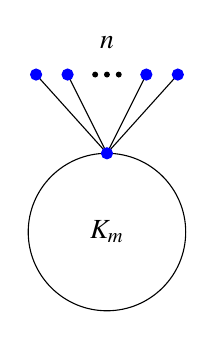
\begin{tikzpicture}[rotate=180] 
   
   \coordinate (c1) at ($(7,0) + (180:1)$);
   \coordinate (c2) at ($(7,0) + (225:1)$);
   \coordinate (c3) at ($(7,0) + (270:1)$);
   \coordinate (c4) at ($(7,0) + (315:1)$);
   \coordinate (c5) at ($(7,0) + (0:1)$);
   \coordinate (c6) at ($(7,0) + (45:1)$);
   \coordinate (c7) at ($(7,0) + (90:1)$);
   \coordinate (c8) at ($(7,0) + (135:1)$);
   
   \coordinate (e1) at ($(7,0) + (270:1) + (0.9,-1.0)$);
   \coordinate (e2) at ($(7,0) + (270:1) + (0.5,-1.0)$);
   \coordinate (e3) at ($(7,0) + (270:1) + (-0.5,-1.0)$);
   \coordinate (e4) at ($(7,0) + (270:1) + (-0.9,-1.0)$);
   
   \coordinate (b1) at ($(7,0) + (270:1) + (0.15,-1.0)$);
   \coordinate (b2) at ($(7,0) + (270:1) + (0,-1.0)$);
   \coordinate (b3) at ($(7,0) + (270:1) + (-0.15,-1.0)$);
   
   \coordinate (lb2) at ($(7,0) + (270:1) + (0,-1.4)$);   
      
  
%   \draw[draw=black] (c1) -- (c2);
%   \draw[draw=black] (c1) -- (c3);
%   \draw[draw=black] (c1) -- (c4);
%   \draw[draw=black] (c1) -- (c5);
%   \draw[draw=black] (c1) -- (c6);
%   \draw[draw=black] (c1) -- (c7);  
%   \draw[draw=black] (c1) -- (c8);
%
%   \draw[draw=black] (c2) -- (c3);
%   \draw[draw=black] (c2) -- (c4);
%   \draw[draw=black] (c2) -- (c5);
%   \draw[draw=black] (c2) -- (c6);
%   \draw[draw=black] (c2) -- (c7);  
%   \draw[draw=black] (c2) -- (c8); 
%
%   \draw[draw=black] (c3) -- (c4);
%   \draw[draw=black] (c3) -- (c5);
%   \draw[draw=black] (c3) -- (c6);
%  \draw[draw=black] (c3) -- (c7);  
%   \draw[draw=black] (c3) -- (c8); 
%
%   \draw[draw=black] (c4) -- (c5);
%   \draw[draw=black] (c4) -- (c6);
%   \draw[draw=black] (c4) -- (c7);  
%   \draw[draw=black] (c4) -- (c8);
%   
%   \draw[draw=black] (c5) -- (c6);
%   \draw[draw=black] (c5) -- (c7);  
%   \draw[draw=black] (c5) -- (c8); 
%
%   \draw[draw=black] (c6) -- (c7);  
%   \draw[draw=black] (c6) -- (c8);  
% 
%   \draw[draw=black] (c7) -- (c8);
    
   \draw[draw=black] (c3) -- (e1);   
   \draw[draw=black] (c3) -- (e2);   
   \draw[draw=black] (c3) -- (e3);   
   \draw[draw=black] (c3) -- (e4);   
   
   %\draw (7,0) circle [radius=1];   
   \draw[black] (7,0) node[circle,minimum size=2cm,draw] (v1) {$K_m$};

   %\filldraw[fill=blue,draw=blue] (c1) circle [radius=0.07];
   %\filldraw[fill=blue,draw=blue] (c2) circle [radius=0.07];
   \filldraw[fill=blue,draw=blue] (c3) circle [radius=0.07];
   %\filldraw[fill=blue,draw=blue] (c4) circle [radius=0.07];
   %\filldraw[fill=blue,draw=blue] (c5) circle [radius=0.07];
   %\filldraw[fill=blue,draw=blue] (c6) circle [radius=0.07];
   %\filldraw[fill=blue,draw=blue] (c7) circle [radius=0.07];
   %\filldraw[fill=blue,draw=blue] (c8) circle [radius=0.07];

   \filldraw[fill=blue,draw=blue] (e1) circle [radius=0.07];
   \filldraw[fill=blue,draw=blue] (e2) circle [radius=0.07];
   \filldraw[fill=blue,draw=blue] (e3) circle [radius=0.07];
   \filldraw[fill=blue,draw=blue] (e4) circle [radius=0.07];
   
   \filldraw[black] (lb2) node {$n$};   
   
   \filldraw[fill=black] (b1) circle [radius=0.03];
   \filldraw[fill=black] (b2) circle [radius=0.03];   
   \filldraw[fill=black] (b3) circle [radius=0.03];
      
\end{tikzpicture}}
}
\endgroup
\end{center}
\caption{The pineapple graph, $PA(m,n)$.}
   \label{fig-pn4}
\end{figure}


\begin{lemma}\label{spectral radius and average degree}
We have $\lambda_1(H) = \frac{n}{2} + c_1\sqrt{n}$ and $\frac{2e(H)}{n} = \frac{n}{4} + c_2\sqrt{n}$, where $|c_1|, |c_2|<1$.
\end{lemma}

\begin{proof}
By eigenvalue interlacing, $\mathrm{PA}(p,q)$ has spectral radius at least $p-1$. A calculation shows 
that for $H = \mathrm{PA}\left( \left\lceil \frac{n}{2}\right\rceil +1, \left\lfloor\frac{n}{2}\right\rfloor-1\right)$, we have 
\[
\lambda_1(H) - \frac{2e(H)}{n} \geq \frac{n}{4} - \frac{3}{2}.
\]
On the other hand, the eigenvector equation gives 
\[
\lambda_1^2 = \sum_{y\sim x} \lambda_1 y = \sum_{y\sim x}\sum_{z\sim y} z \leq \sum_{y\sim x}d_y \leq 2e(G) - (n-1),
\]
where the last inequality follows because $G$ is connected. This gives
\begin{equation}\label{lower bound on average degree}
d \geq \frac{\lambda_1^2}{n} + 1 - \frac{1}{n}.
\end{equation}
Setting $\lambda_1 = pn$ and applying \eqref{lower bound on average degree}, we have $\lambda_1 - d \leq pn - p^2n -1 + \frac{1}{n}$. The right hand side of the inequality is maximized at $p=1/2$, giving 
\begin{equation}\label{tight bound on irregularity}
\frac{n}{4} - \frac{3}{2} \leq \lambda_1 - d \leq \frac{n}{4} - 1 + \frac{1}{n}.
\end{equation}

Next setting $\lambda_1 = \frac{n}{2} + c_1 \sqrt{n}$, \eqref{lower bound on average degree} gives
\[
d \geq \frac{n}{4} + c_1\sqrt{n} + c_1^2 + 1 - \frac{1}{n},
\]
whereas \eqref{tight bound on irregularity} gives
\begin{equation}\label{d bar bound}
d \leq \lambda_1 - \frac{n}{4} + \frac{3}{2}  = \frac{n}{4} + c_1\sqrt{n}  + \frac{3}{2}.
\end{equation}
Together, these imply $|c_1| <1$ and prove both statements for $n$ large enough.
\end{proof}

\begin{lemma}\label{error in x neighborhood small}
There exists a constant $c_3$ not depending on $n$ such that 
\[
0 \leq \frac{1}{|N(x)|} \sum_{y\sim x} d_y - \lambda_1 y \leq c_3\sqrt{n}.
\]
\end{lemma}

\begin{proof}
By the eigenvector equation
\[
\sum_{y\sim x} \lambda_1 y = \lambda_1^2 = \sum_{y\sim x}\sum_{z\sim y} z \leq \sum_{y\sim x} d_y \leq dn - (n-1).
\]
Rearranging and applying Lemma \ref{spectral radius and average degree}, we have
\[
0\leq \sum_{y\sim x} \left( d_y - \lambda_1 y \right) = O\left(n^{3/2}\right).
\]
By the eigenvector equation again, and because the first eigenvector is normalized with $x=1$, we have
\[
\lambda_1 = \sum_{y\sim x} y \leq d_x,
\]
giving $d_x = \Omega(n)$. Combining, we have 
\[
\frac{1}{|N(x)|} \sum_{y\sim x} \left( d_y - \lambda_1 y \right) = O\left(\sqrt{n}\right),
\]
where the implied constant is independent of $n$.
\end{proof}

Now we fix a constant $\epsilon > 0$, whose exact value will be 
chosen later.  The next lemma implies that close to half of the vertices of
$G$ have eigenvector entry close to $1$ for $n$ sufficiently large, 
depending on the chosen $\epsilon$.  We follow that with a proposition
which outlines the approximate structure of $G$, and then finally use
variational arguments to deduce that $G$ is exactly a pineapple graph.


\begin{lemma}\label{u good}
 There exists a vertex $u\not=x$ with $u > 1- 2 \epsilon$ and $d_u - \lambda_1 u = O(\sqrt{n})$.  Moreover $d_u \geq \left( 1/2 - 2\epsilon \right)n$.
\end{lemma}


%\begin{lemma}\label{y good}
%Let $\epsilon >0$. There exists a $y\in N(x)$ such that $y> \frac{1}{2} - \epsilon$ and $d_y - \lambda_1 y < c_\epsilon \sqrt{n}$ where $c_\epsilon$ is a constant depending only on $\epsilon$.
%\end{lemma}

\begin{proof}
We proceed by first showing a weaker result: that there is a vertex $y$ with
$y> \frac{1}{2} - \epsilon$ and $d_y - \lambda_1 y = O(\sqrt{n})$, and 
additionally that $y \in N(x)$.  We will use then use this to bootstrap
the required result.


Let $A: = \{z\sim x: z> \frac{1}{2} - \epsilon\}$. By Lemma \ref{spectral radius and average degree},
\[
\lambda_1 = \frac{n}{2} + c_1\sqrt{n}
\]
where $|c_1| <1$. Since $0< z\leq 1$ for all $z\sim x$, we have that $|A| \geq \delta_\epsilon n$ where $\delta_\epsilon$ is a positive constant that depends only on $\epsilon$. Let $B = \{z\sim x: d_z - \lambda_1 z >  K\sqrt{n}\}$, where $K$ is a fixed constant whose exact value will be chosen later. Now
\[
\frac{1}{|N(x)|} \sum_{y\sim x} \left( d_y -\lambda_1 y \right) \geq \frac{1}{|N(x)|} \sum_{z\in B} \left( d_z - \lambda_1 z \right) \geq \frac{1}{n} |B| K\sqrt{n}.
\]
By Lemma \ref{error in x neighborhood small}, $|B| \leq \frac{c_3}{K} n$. Therefore, for $K$ large enough depending only on $\epsilon$, we have $\left|A\cap B^c\right| > 0$.  This proves the existence of the vertex $y$,
with the properties claimed at the beginning of the proof.


Next, we show that there exists a set $U\subset N(y)$ such that 
$|U| \geq \left(\frac{1}{4} - 2\epsilon \right)n$ and 
$u \geq 1-2\epsilon$ for all $u\in U$.  By Lemma \ref{spectral radius and average degree},
\[
\left(\frac{n}{2} + c_1\sqrt{n}\right)\left(\frac{1}{2} - \epsilon\right) \leq \lambda_1 y \leq d_y,
\]
where $|c_1| < 1$. So $d_y \geq \left(\frac{1}{4} - \epsilon \right) n$ for $n$ large enough. Now let $C = \{z\sim y: z < 1-2\epsilon \}$. Then
\[
K \sqrt{n} \geq d_y - \lambda_1 y = \sum_{z\sim y} \left( 1 - z \right) \geq \sum_{z\in C} \left( 1-z \right) \geq 2|C| \epsilon.
\]
Therefore
\[
|N(y) \setminus C| \geq \left(\frac{1}{4} - \epsilon\right)n  - \frac{K \sqrt{n}}{2\epsilon}.
\]
Setting $U = N(y) \setminus C$, we have $|U| > \left(\frac{1}{4} - 2\epsilon\right)n$ for $n$ large enough. 


Set $D = U \cap N(x)$.  We will first find a lower bound on $|D|$.  We have
 \begin{equation*}
  \lambda_1^2 \leq \sum_{y \sim x} d_y \leq 2m - \sum_{y \not \in N(x)} d_y
 \end{equation*}
Rearranging this we get 
 \[ d - \frac{\lambda_1^2}{n} \geq \frac{1}{n} \sum_{y \not \in N(x)} d_y\]
Now applying the bound on $d$ from equation~\ref{d bar bound} and expression for $\lambda_1$ in Lemma~\ref{spectral radius and average degree} yields
 \[ \left( \frac{n}{4} + c_1 \sqrt{n} + \frac{3}{2}\right) - \frac{\left(\frac{n}{2} + c_1 \sqrt{n}\right)^2}{n} \geq \frac{1}{n} \sum_{y \not \in N(x)} d_y \]
which implies that
 \[ \frac{3}{2} n \geq \left( \frac{3}{2} - c_1^2 \right) n \geq \sum_{y \not \in N(x)} d_y \geq \sum_{y \in U\setminus N(x)} d_y \geq |U\setminus N(x)| (1-2\epsilon) \lambda_1 .\]
So 
 \[ |U \setminus N(x)| \leq \frac{3}{2(1-2\epsilon)} \frac{n}{\lambda_1} = \frac{3}{2(1-2\epsilon)} \frac{1}{1/2 + c_1 n^{-1/2}} .\]
In particular, $|D| \geq (\frac{1}{4} - c'_\epsilon) n$.

Now by the same argument used at the start of the proof to show the existence
of the vertex $y$, we have some vertex $u \in D$
with $d_u - \lambda_1 u = O(\sqrt{n}$).   Finally 
\[d_u \geq u \lambda_1 \geq (1 - 2 \epsilon) (n/2 + c_1\sqrt{n}) \geq \left( 1/2 - 2\epsilon \right)n .  \]

\end{proof}

\subsection{Alteration Step}

\begin{lemma}\label{modifying conditions}
 Let $x,y$ be two vertices in $G$.  If
 $xy > 1/2 +n^{-1/2} + 5n^{-1}$, then $x$ and $y$ are adjacent.  On the
 other hand, if $xy < 1/2 - 3\epsilon$ then $x$ and $y$ are not adjacent.
\end{lemma}
\begin{proof}
We begin by bounding the dot product of the leading eigenvector $\textbf{v}$
with itself, we will show that
\begin{equation}\label{vvt bound}
\frac{n}{2} + \sqrt{n} + 5 \geq \textbf{v}^t\textbf{v} > \frac{n}{2} - 2 \epsilon n  - O(\sqrt{n})
\end{equation}


\noindent First, we show the lower bound.  With $u$ from the previous lemma, by Cauchy--Schwarz we have
\[  \textbf{v}^t\textbf{v} \geq \sum_{z \sim u} z^2 \geq \frac{1}{d_u}\left( \sum_{z \sim u} z \right)^2 = \frac{(\lambda_1 u)^2}{d_u} \]
By Lemma~\ref{u good}, we then have
 \[\textbf{v}^t\textbf{v} \geq \frac{(d_u - O(\sqrt{n}))^2}{d_u} \geq d_u - O(\sqrt{n}) > \frac{n}{2} - 2 \epsilon n  - O(\sqrt{n}) .\]
For the upper bound of inequality~\eqref{vvt bound}, first set $E = \left( N(x) \cup \{x\}\right)^C$.  Then
 \[ \textbf{v}^t\textbf{v} = \sum_{z \in V(G)} z^2 \leq \sum_{z \in V(G)} z \leq 1 + \sum_{z \in N(x)} z + \sum_{z \in E} z \leq 1 + \lambda_1 + \frac{1}{\lambda_1} \sum_{z \in E} d_z .\]
From the proof of Lemma~\ref{u good} we have the bound
 \[ \sum_{ z \in E} d_z \leq \frac{3}{2} n .\]
Hence
 \[ \textbf{v}^t \textbf{v}  \leq 1 + \frac{n}{2} + c_1 \sqrt{n} + \frac{3}{2} \cdot \frac{1}{1/2 + c_1 n^{-1/2}} \leq \frac{n}{2} + \sqrt{n} + 5 .\]
This completes the proof of inequality~\eqref{vvt bound}.


 Let $\lambda_1^+$ be the leading eigenvalue of the graph formed by adding the 
 edge $\{x,y\}$ to $G$.  Then by \eqref{rayleigh quotient} we have
  \[ \lambda_1^+ - \lambda_1 \geq \frac{\textbf{v}^t (A^+-A) \textbf{v}}{\textbf{v}^t \textbf{v}} \geq \frac{2xy}{\textbf{v}^t \textbf{v}} \geq \frac{2xy}{n/2 + \sqrt{n} + 5}  = \frac{2xy}{n(1/2+n^{-1/2} + 5 n^{-1})}.\]
If $xy > 1/2+n^{-1/2} + 5n^{-1}$, then
\[ (\lambda_1^+ - d^+) - (\lambda - d) > \frac{2}{n} - \frac{2}{n} \geq 0\]
Hence $\left\{x,y\right\}$ must already have been an edge, otherwise this
would contradict the maximality of $G$.

Similarly if $\lambda_1^-$ is the leading eigenvalue of the graph obtained
from $G$ by deleting the edge $\{x,y\}$, then  
  \[ \lambda_1 - \lambda_1^- \leq \frac{\textbf{v}^t (A-A^-) \textbf{v}}{\textbf{v}^t \textbf{v}} \leq \frac{2xy}{n/2 - 2\epsilon n - O(\sqrt{n})} \leq \frac{2xy}{(1/2 - 3 \epsilon)n}\]
when $n$ is large enough.  Now if
$xy < 1/2 - 3\epsilon$, then 
 \[ (\lambda_1 - d) - (\lambda_1^- - d^-) < 0 .\] %XXX: this doesn't typeset well

\end{proof}

%%%%%%%%%%%%%%%%%%picture%%%%%%%%%%%%%

\begin{figure}[]
\begin{center}
\begingroup

\setlength{\unitlength}{.01cm}
{
\setlength{\fboxsep}{10pt}
\framebox[1.5\width]{
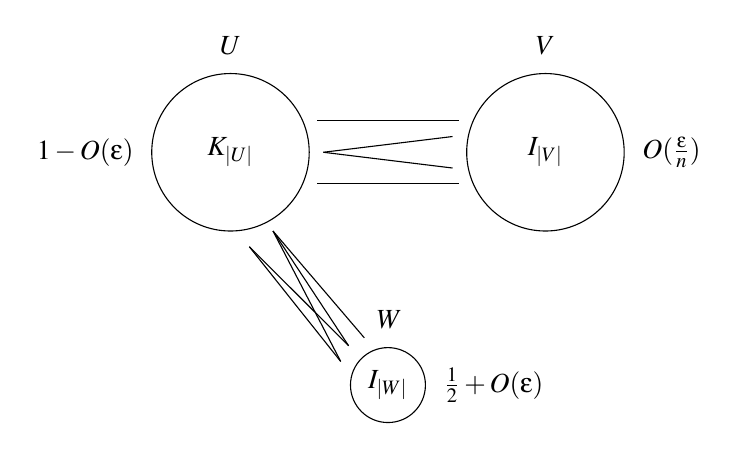
\begin{tikzpicture}
\filldraw[black] (0.553380,1.150606) node[label={[label distance=0.1cm]180:$1 - O(\epsilon)$},label={[label distance=0.1cm]$U$},circle,minimum size=2cm,draw] (v0) {$K_{|U|}$};

\filldraw[black] (4.553380,1.150606) node[label={[label distance=0.1cm]0:$O(\frac{\epsilon}{n})$},label={[label distance=0.1cm]$V$},circle,minimum size=2cm,draw] (v1) {$I_{|V|}$};

\filldraw[black] (2.553380,-1.80606) node[label={[label distance=0.1cm]0:$\frac{1}{2}+O(\epsilon)$},label={[label distance=0.1cm]88:$W$},circle,minimum size=0.8cm,draw] (v1) {$I_{|W|}$};

\coordinate (UC) at (0.553380,1.150606);
\coordinate (VC) at (4.553380,1.150606);
\coordinate (WC) at (2.553380,-1.80606);

\coordinate (Ul1) at ($(UC) + (1.1,-0.4)$);
\coordinate (Ul2) at ($(UC) + (1.18,-0)$);
\coordinate (Ul3) at ($(UC) + (1.1,0.4)$);

\coordinate (Ub2) at ($(UC) + (0.24,-1.2)$);
\coordinate (Ub3) at ($(UC) + (0.54,-1.0)$);


\coordinate (Vl1) at ($(VC) + (-1.1,-0.4)$);
\coordinate (Vl2a) at ($(VC) + (-1.18,-0.2)$);
\coordinate (Vl2b) at ($(VC) + (-1.18,0.2)$);
\coordinate (Vl3) at ($(VC) + (-1.1,0.4)$);

\coordinate (Wt1) at ($(WC) + (-0.5,0.5)$);
\coordinate (Wt2) at ($(WC) + (-0.3,0.6)$);
\coordinate (Wt3) at ($(WC) + (-0.6,0.3)$);


\draw (Ul1) -- (Vl1);
\draw (Ul2) -- (Vl2a);
\draw (Ul2) -- (Vl2b);
\draw (Ul3) -- (Vl3);

\draw (Ub3) -- (Wt1);
\draw (Ub3) -- (Wt2);
\draw (Ub3) -- (Wt3);

\draw (Ub2) -- (Wt3);
\draw (Ub2) -- (Wt1);

%\draw[black] (v0) -- (v1);

\end{tikzpicture}}
}
\endgroup
\end{center}
\caption{Structure of $G$ in Proposition \ref{almost pineapple structure}.  The number beside
each set indicates the values of eigenvector entries in the set. 
$U$ is a clique, $V$, $W$ are independent sets.  Vertices in $V$ are adjacent
to one vertex in $U$, and vertices in $W$ are adjacent to multiple vertices in $U$.
   \label{pineapple structure picture}}
\end{figure}

%%%%%%%%%%%%%%%%%%%%%%%%

\begin{proposition}\label{almost pineapple structure}
For $n$ sufficiently large, we can partition the vertices of $G$ into three 
sets $U, V, W$ (see Figure \ref{pineapple structure picture}) where 
\begin{itemize}
 \item[(i)] vertices in $V$ have eigenvector entry smaller than $(2+\epsilon) / n$ and have degree one, 
 \item[(ii)] vertices in $U$ induce a clique, 
 all have eigenvector entry larger than $1 - 20\epsilon$, and $(1/2 - 3\epsilon) n \leq |U| \leq (1/2 + \epsilon)n$,

 \item[(iii)] vertices in $W$ have eigenvector entry in the range $\left[1/2 - 4\epsilon,  1/2 + 21 \epsilon \right]$ and are adjacent only to vertices in $U$.  
\end{itemize}
\end{proposition}

\begin{proof}
  By Lemma~\ref{modifying conditions}, any two vertices in $G$ with eigenvector entry $1$ are adjacent.  Moreover, it is easy to see that
  every vertex in $G$ is incident to at least one vertex with eigenvector entry $1$:  if not, for each vertex not incident to a vertex
  with eigenvector entry $1$, delete one of its edges and add a new edge from that vertex to a vertex with eigenvector entry $1$ (such as
  the vertex $x$).  The resulting graph is connected, will have the same number of edges as the original graph, and will have strictly larger $\lambda_1$
  (this can be seen by considering the Rayleigh quotient, as in the proof of Lemma~\ref{modifying conditions}).
  So by maximality of $G$, there are no such vertices.  This implies that the set of edges that are incident
  to a vertex with eigenvector entry $1$ spans the vertex set of $G$. 
  In particular, if we remove any edge that is not incident to a vertex with eigenvector entry $1$, we do not disconnect the graph.  We will use this fact repeatedly in this proof.

 
  
\begin{itemize}
\item[(i)] Let $V$ consist of all vertices in $G$ with eigenvector entry 
less than $1/2 - 4 \epsilon$.  By Lemma~\ref{modifying conditions}, removing 
any edge incident to a vertex in $V$ strictly increases $\lambda_1 - d$, so each vertex in $V$ has degree one.  By the eigenvector equation,
the eigenvector entry of any such vertex is at most $1/\lambda_1 < (2+\epsilon) / n $, when $n$ is large enough.
\item[(ii)] From Lemma~\ref{u good}, we have a vertex $u$ such that $d_u - \lambda_1 u = O(\sqrt{n})$.  Let $X$ be the set of neighbors $z$ of $u$ such that $z < 9/10$.  Then we have
 \[ (1 - 9/10)|X| \leq \sum_{y \sim u} 1 - y = d_u - \lambda_1 u = O(\sqrt{n}). \]
Hence $|X| = O(\sqrt{n})$.  Let $U$ be all vertices in $G$ with eigenvector entry at least $9/10$.  So, by Lemma~\ref{u good}
 \[ |U| \geq d_u - |X| \geq n/2 - 2 \epsilon n - O(\sqrt{n})\]
For $n$ large enough, we have $|U| \geq (1/2 - 3\epsilon) n$. For sufficiently large $n$, by Lemma~\ref{modifying conditions} these vertices are all adjacent to each other.  For the upper bound on $|U|$ we use the expression for $e(G)$ in Lemma~\ref{spectral radius and average degree}
\[ |U| (|U| - 1) \leq 2e(G) \leq  \frac{n^2}{4} + c_2n\sqrt{n}\]
which implies $|U| \leq (1/2+\epsilon) n$ for large enough $n$.

Now take any vertex $y \in U$.  If $x$ is a vertex with largest eigenvector entry, then 
\begin{equation}\label{y_bound}
 \lambda_1 - \lambda_1 y \leq \sum_{z \in N(x) \setminus N(y)} z \leq y + \sum_{z \in U^C} z 
\end{equation}
We have
 \begin{eqnarray*}
  \lambda_1 \sum_{z \in U^C} z \leq \sum_{z \in U^C} d_z &\leq& 2e(G) - 2|E(U,U)|\\
   &\leq& \frac{n^2}{4} + c_2 n \sqrt{n} - (1/2 - 3\epsilon)(1/2 - 3 \epsilon - 1/n) n^2 \\
   &\leq & 4 \epsilon n^2
 \end{eqnarray*}
for $n$ sufficiently large, where we are using the expression for $e(G)$ given by Lemma~\ref{spectral radius and average degree}.
In particular,
 \[ \sum_{z \in U^C} z \leq 9 \epsilon n \] 
Finally, by equation~\ref{y_bound} we have 
 \[ y \geq 1 - \frac{1}{\lambda_1} \sum_{z \in U^C} z -\frac{y}{\lambda_1} \geq (1 - 20 \epsilon) .\]
 
\item[(iii)] Let $W$ consist of all remaining vertices of $G$.  If a vertex 
has eigenvector entry smaller than $1/2 - 4\epsilon$ then it is in $V$ by
construction.  If a vertex $z \in W$ has eigenvector entry larger than $1/2 + 21\epsilon$
then we have
 \[ (1/2 + 21 \epsilon) (1 - 20 \epsilon) > 1/2 + \epsilon \]
if $\epsilon < 1/50$, say.   So for sufficiently large $n$, by Lemma~\ref{modifying conditions} we 
have that $z$ is adjacent to every vertex in $U$.  But by the proof of part (ii), this implies that $z > 1 - 20\epsilon$, which contradicts $z \in W$.

For $z \in W$ and any vertex $y \in U^C$, then 
 $yz \leq (1/2 + 21 \epsilon)(1/2 + 21\epsilon) < 1/4 + 22 \epsilon$
and so by Lemma~\ref{modifying conditions} there is no edge between $y$ and 
$z$ in the maximal graph $G$.
\end{itemize}
\end{proof}

\subsection{The Pineapple Graph is Extremal}

\begin{theorem}
For sufficiently large $n$, $G$ is a pineapple graph.
\end{theorem}
\begin{proof}
Take $U,V,W$ as in the previous lemma.  We begin by showing that the set $W$ must be empty.  Assume to the contrary, and let $z$ be in $W$, and furthermore
let $G^+$ be the graph obtained by adding edges from $z$ to every vertex in $U$.
We will show that $\lambda_1(G^+) - d(G^+) > \lambda_1(G) - d(G)$, which contradicts the maximality of $G$.

Since the vertex $z$ is adjacent only to vertices in $U$, and the
fact that vertices in $U$ have eigenvector entry between $1-20\epsilon$ and $1$,
the eigenvector equation yields
 \[\lambda_1 (1/2 - 4 \epsilon) \leq \lambda_1 z \leq d_z(G) \leq \frac{\lambda_1 z}{1 - 20 \epsilon} = (1/2 + O(\epsilon))\lambda_1\]

\noindent Using the expression for $\lambda_1$ in Lemma~\ref{spectral radius and average degree}, for large enough $n$ we have
 \[ \left(1-\epsilon\right)\frac{n}{4} \leq d_z(G) \leq \left(1+\epsilon\right) \frac{n}{4}\]
So we can bound the change in the average degrees
 \[ d(G^+) - d(G) \leq \frac{2(|U| - (1-\epsilon)n/4)}{n}< 1/2 + 3\epsilon\]
Next we find a lower bound on $\lambda_1(G^+) - \lambda_1(G)$.  Recall that $\textbf{v}$
is the leading eigenvector of $A(G)$, normalized so that $||\textbf{v}||_\infty = 1$.  Let $\textbf{w}$ be the vector that is equal to $\textbf{v}$ on all 
vertices except $z$, and equal to $1$ for $z$.  Then, 
 \[ \lambda_1(G^+) \geq \frac{\textbf{w}^tA^+\textbf{w}}{\textbf{w}^t\textbf{w}}\] 
We first find a lower bound for the numerator (with abuse of big-O notation with inequalities)
\begin{eqnarray*} 
\textbf{w}^tA^+\textbf{w} & \geq & \textbf{w}^tA\textbf{w} + 2(|U| - d_z(G))(1-O(\epsilon)) \geq \textbf{w}^tA\textbf{w} + (1/2-O(\epsilon))n \\
& \geq &  \textbf{v}^tA\textbf{v} + 2d_z(G) \left(1-z\right)(1-20\epsilon) + (1/2-O(\epsilon))n \\
%& \geq &  \textbf{v}^tA\textbf{v} + 2d_z(G) \left(1/2 - 21\epsilon\right)(1-20\epsilon) + (1/2-O(\epsilon))n \\
& \geq &  \textbf{v}^tA\textbf{v} + 2d_z(G) \left(1/2 - 31\epsilon\right) + (1/2-O(\epsilon))n \\
%& \geq & \textbf{v}^tA\textbf{v} + 2(1-\epsilon)(n/4) \left(1/2 - 31\epsilon\right) + (1/2-O(\epsilon))n \\
%& \geq & \textbf{v}^tA\textbf{v} + (n/4) \left(1 - 63\epsilon\right) + (1/2-O(\epsilon))n\\
& \geq &  \textbf{v}^tA\textbf{v} + (3/4-O(\epsilon))n
\end{eqnarray*}
Similarly, we find an upper bound for the denominator
\begin{eqnarray*}
\textbf{w}^t \textbf{w} &=& \textbf{v}^t\textbf{v} + 1 - z^2 \\
&\leq& \textbf{v}^t\textbf{v} + 1 - (1/2 - 4\epsilon)^2 \\
&\leq& \textbf{v}^t\textbf{v} + 3/4 + 4\epsilon
\end{eqnarray*}
Combining these, and using the bound on $\textbf{v}^t\textbf{v}$ from
the proof of Lemma~\ref{modifying conditions}, we get
\begin{eqnarray*}
 \lambda_1(G^+) - \lambda_1(G) &\geq& \frac{\textbf{w}^tA^+\textbf{w}}{\textbf{w}^t\textbf{w}} - \frac{\textbf{v}^tA\textbf{v}}{\textbf{v}^t\textbf{v}}\\
% & \geq & \frac{\textbf{v}^tA\textbf{v} + (1-37\epsilon)3n/4}{\textbf{v}^t\textbf{v} + 3/4 + 4\epsilon} -  \frac{\textbf{v}^tA\textbf{v}}{\textbf{v}^t\textbf{v}}\\
 &\geq& \frac{\textbf{v}^t\textbf{v}(3/4-O(\epsilon))n - \textbf{v}^tA\textbf{v} (3/4 + 4\epsilon)}{\textbf{v}^t\textbf{v} (\textbf{v}^t\textbf{v} + 3/4 + 4\epsilon)}\\
 &\geq & \frac{(3/4-O(\epsilon))n - (3/4 + 4\epsilon)\lambda_1(G)}{\textbf{v}^t\textbf{v} + 3/4 + 4\epsilon} \\ 
 &= &  3/4 + O(\epsilon)
\end{eqnarray*}
Hence $\lambda_1(G^+) - \lambda_1(G) > d(G^+) - d(G)$, and by maximality of $G$ we conclude that $W = \emptyset$.

At this point we know that $G$ consists of a clique together with a set of pendant vertices $V$.  All that remains is to show that all of the pendant vertices  are incident to the same vertex in the clique.  Let $V = \left\{v_1, v_2, \cdots, v_k\right\}$, and let $u_i$ be the unique vertex in $U$ that $v_i$ is adjacent to.  Let $G^+$ be the graph obtained from $G$ by deleting the edges $\left\{v_i,u_i\right\}$ and adding the edges $\left\{v_i,x\right\}$, where $x$ is a vertex with eigenvector entry $1$.  Now, $d(G^+) = d(G)$, and 
\[ \lambda_1(G^+) -\lambda_1(G) \geq \frac{\textbf{v}^t A^+ \textbf{v}}{\textbf{v}^t\textbf{v}} - \frac{\textbf{v}^t A \textbf{v}}{\textbf{v}^t\textbf{v}}\]
with equality if and only if $\textbf{v}$ is a leading eigenvector for $A^+$.  We have
\[\frac{\textbf{v}^t A^+ \textbf{v}}{\textbf{v}^t\textbf{v}} - \frac{\textbf{v}^t A \textbf{v}}{\textbf{v}^t\textbf{v}} = \frac{1}{\textbf{v}^t\textbf{v}}\left( \sum_{i=1}^k 1 - u_i \right) \geq 0\]
with equality if and only if $u_i = 1$ for all $1 \leq i \leq k$.  By maximality of $G$, we have equality in both of the above inequalities, and so $\textbf{v}$ is a leading eigenvector for $G^+$, and every vertex in $U$ incident to a vertex in $V$ has eigenvector entry 1.  $G^+$ is a pineapple graph, and it is easy to see that there is a single vertex in a pineapple graph with maximum eigenvector entry.  It follows that the vertices in $V$ are all adjacent to the same vertex in $U$, and hence $G$ is a pineapple graph.

\end{proof}


This chapter is based on the papers ``Three conjectures in extremal spectral graph theory'',
 \cite{TaitTobin2017}, to appear in \textit{Journal of Combinatorial Theory, Series B},
 and ``Characterizing graphs of maximum principal ratio'', submitted to
 \textit{Electronic Journal of Linear Algebra} \cite{TaitTobin2015},
both written jointly with Michael Tait.  The dissertation
author was the primary investigator and author of the paper.


\chapter{The Spectral Radius of Outerplanar and Planar Graphs}
\section{Introduction}

The study of spectral radius of planar graphs has a long history, dating back to at least Schwenk
and Wilson \cite{SchwenkWilson1978}.  This direction
of research was further motivated by applications where the spectral
radius is used as a measure of the connectivity of a network, in
particular for planar
networks in areas such as geography, see for example \cite{BootsRoyle1991}
and its references.  To compare connectivity of networks to a theoretical upper bound, geographers were
interested in finding the planar graph of maximum spectral radius. To this end, Boots and Royle and
independently Cao and Vince conjectured that the extremal graph is $P_2 + P_{n-2}$
\cite{BootsRoyle1991}, \cite{CaoVince1993}. Several researchers have worked on this problem and
successively improved upon the best theoretical upper bound, including \cite{Hong1988},
\cite{CaoVince1993}, \cite{Hong1995}, \cite{Guiduli1996}, \cite{Hong1998},
\cite{EllinghamZha2000}. Other related problems have been considered, for example Dvo\v{r}\'{a}k
and Mohar found an upper bound on the spectral radius of planar graphs
with a given maximum degree \cite{DvorakMohar2010}. Work has also been done maximizing the spectral radius of graphs on surfaces of higher genus \cite{EllinghamZha2000, Hong1995, Hong1998}. We would also like to note that it is claimed in \cite{EllinghamZha2000} that Guiduli and Hayes proved
that the maximum spectral radius of a planar graph is attained by $P_2 + P_{n-2}$,
for sufficiently large $n$. However, this preprint has never appeared, and the authors
could not be reached for comment on it.


The outerplanar conjecture appeared
in \cite{CvetkovicRowlinson1990}, where the authors mention that it is related
to the study of various subfamilies of Hamiltonian graphs.
Rowlinson \cite{Rowlinson1990} made partial progress on this conjecture, which
was also worked on by Cao and Vince \cite{CaoVince1993} and Zhou--Lin--Hu \cite{ZhouLinHu2001}.

% TODO: introduce method by giving proof of Mantel

% TODO: introduce notation

\section{Outerplanar Graphs of Maximum Spectral Radius}\label{outerplanar}
Let $G$ be a graph. As before, let the first eigenvector of the adjacency matrix of $G$ be $\textbf{v}$ normalized so that maximum entry is $1$. For $v\in V(G)$ we will use $v$ to mean a vertex or the eigenvector entry of that vertex, where it will be clear from context which meaning we are using. Let $x$ be a vertex with maximum eigenvector entry, ie $x=1$.  Throughout let $G$ be an outerplanar graph on $n$ vertices with maximal adjacency spectral radius.  $\lambda_1$ will refer to $\lambda_1(A(G))$. 

Two consequences of $G$ being outerplanar that we will use frequently are that $G$ has at most $2n-3$ edges and $G$ does not contain $K_{2,3}$ as a subgraph. An outline of our proof is as follows. We first show that there is a single vertex of large degree and that the remaining vertices have small eigenvector entry (Lemma \ref{small eigvec}). We use this to show that the vertex of large degree must be adjacent to every other vertex (Lemma \ref{bound bad elements}). From here it is easy to prove that $G$ must be $K_1+P_{n-1}$.

\begin{figure}[]
\begin{center}
\begingroup

\setlength{\unitlength}{.01cm}
{
\setlength{\fboxsep}{10pt}
\framebox[1.5\width]{
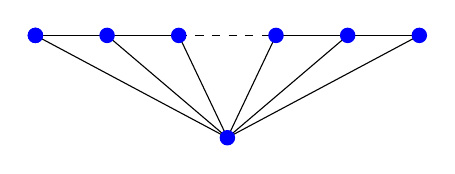
\begin{tikzpicture}[rotate=90, scale=1.3]


\coordinate (W) at (1.553380,0.70606);

\coordinate (W1) at ($(W) + 0*(0,-0.7)$);
\coordinate (W2) at ($(W) + 1*(0,-0.7)$);
\coordinate (W3) at ($(W) + 2*(0,-0.7)$);
\coordinate (W4) at ($(W) + 3*(0,-0.7) + (0,-0.25)$);
\coordinate (W5) at ($(W) + 4*(0,-0.7) + (0,-0.25)$);
\coordinate (W6) at ($(W) + 5*(0,-0.7) + (0,-0.25)$);


\coordinate (B) at ($0.5*(W3) + 0.5*(W4) + (-1.0,0)$);


\draw (W1) -- (W2);
\draw (W2) -- (W3);
\draw [dashed] (W3) -- (W4);
\draw (W4) -- (W5);
\draw (W5) -- (W6);

\draw (B) -- (W1);
\draw (B) -- (W2);
\draw (B) -- (W3);
\draw (B) -- (W4);
\draw (B) -- (W5);
\draw (B) -- (W6);

\filldraw[blue] (W) circle (0.07cm);
\filldraw[blue] (W1) circle (0.07cm);
\filldraw[blue] (W2) circle (0.07cm);
\filldraw[blue] (W3) circle (0.07cm);
\filldraw[blue] (W4) circle (0.07cm);
\filldraw[blue] (W5) circle (0.07cm);
\filldraw[blue] (W6) circle (0.07cm);

\filldraw[blue] (B) circle (0.07cm);

\end{tikzpicture}}
}
\endgroup
\end{center}
\caption{The graph $P_1 + P_{n-1}$.
   \label{fig-pn4}}
\end{figure}


We begin with an easy lemma that is clearly not optimal, but suffices for our needs.
\begin{lemma}\label{trivial lambda bound}
 $\lambda_1 > \sqrt{n-1}$.
\end{lemma}
\begin{proof}
 The star $K_{1,n-1}$ is outerplanar, and cannot be the maximal outerplanar
 graph with respect to spectral radius because it is a strict subgraph of other outerplanar graphs on the same vertex set.  Hence, $\lambda_1(G) > \lambda_1(K_{1,n}) = \sqrt{n-1}$.
\end{proof}

\begin{lemma}
 For any vertex $u$, we have $d_u > un - 11\sqrt{n}$.
\end{lemma}
\begin{proof}
 Let $A$ be the neighborhood of $u$, and let $B = V(G) \setminus (A\cup \{x\})$.  We have 
  \[ \lambda_1^2 u = \sum_{y \sim u} \sum_{z \sim y} z \leq d_u + \sum_{y \sim u} \sum_{z \in N(y)\cap A} z + \sum_{y \sim u} \sum_{z \in N(y)\cap B} z \]

\noindent By outerplanarity, each vertex in $A$ has at most two neighbors in $A$, otherwise
$G$ would contain a $K_{2,3}$.  In particular,
 \[ \sum_{y \sim u} \sum_{z \in N(y)\cap A} z  \leq 2 \sum_{y \sim u} y = 2\lambda_1 u \]
Similarly, each vertex in $B$ has at most $2$ neighbors in $A$.  So
 \[ \sum_{y \sim u} \sum_{z \in N(y)\cap B} z \leq 2 \sum_{z \in B} z \leq \frac{2}{\lambda_1} \sum_{z \in B} d_z \leq \frac{4e(G)}{\lambda_1} \leq \frac{4(2n-3)}{\lambda_1}\]
as  $e(G) \leq 2n-3$ by outerplanarity.  So, using Lemma~\ref{trivial lambda bound} we have
 \[ \sum_{y \sim u} \sum_{z \in N(y)\cap B} z < 8 \sqrt{n}\]
Combining the above inequalities yields
 \[ \lambda_1^2 u - 2\lambda_1 u < d_u + 8 \sqrt{n}\]
Again using Lemma~\ref{trivial lambda bound} we get
 \[ un - 11\sqrt{n} <  (n-1 - 2\sqrt{n-1}) u - 8 \sqrt{n} < d_u .\]
\end{proof}

\begin{lemma}\label{small eigvec}
 We have $d_x > n - 11 \sqrt{n}$ and for every other vertex $u$, $u < C_1 / \sqrt{n}$ for some absolute constant $C_1$, for $n$ sufficiently large.
\end{lemma}
\begin{proof}
The bound on $d_x$ follows immediately from the previous lemma and the normalization that
$x=1$.  Now consider any other vertex $u$.  We know that $G$ contains no $K_{2,3}$, so $d_u < 12 \sqrt{n}$, otherwise $u,x$ share $\sqrt{n}$ neighbors, which
yields a $K_{2,3}$ if $n \geq 9$.  So
 \[ 12 \sqrt{n} > d_u > u n - 11\sqrt{n}, \]
that is, $u < 23 / \sqrt{n}$.
\end{proof}

\begin{lemma}\label{bound bad elements}
 Let $B = V(G) \setminus (N(x) \cup \{x\})$.  Then
  \[ \sum_{z \in B} z < C_2 / \sqrt{n} \]
 for some absolute constant $C_2$.
\end{lemma}
\begin{proof}
From the previous lemma, we have that $|B| < 11 \sqrt{n}$.  Now
 \[ \sum_{z \in B} z \leq \frac{1}{\lambda_1} \sum_{z \in B} \left(23 / \sqrt{n}\right) d_z = \frac{23}{\lambda_1 \sqrt{n}} \left( e(A,B) + 2 e(B)\right) \]
Each vertex in $B$ is adjacent to at most two vertices in $A$, so $e(A,B) \leq 2 |B| < 24 \sqrt{n}$.  The graph induced on $B$ is outerplanar, so
$e(B) \leq 2|B| - 3 < 24 \sqrt{n}$.  Finally, using the fact that $\lambda_1 > \sqrt{n-1}$, we get the required result.
\end{proof}

\begin{theorem}
 For sufficiently large $n$, $G$ is the graph $K_1 + P_{n-1}$, where $+$ represents the graph join operation.
\end{theorem}
\begin{proof}
First we show that the set $B$ above is empty, ie. $x$ is adjacent
to every other vertex.  If not, let $y \in B$.  Now $y$ is adjacent to at
most two vertices in $A$, and so by Lemma~\ref{small eigvec} and Lemma~\ref{bound bad elements}, 
 \[ \sum_{z \sim y} z < \sum_{z \in B} z + 2 C_1 / \sqrt{n} < (C_2 + 2 C_1) / \sqrt{n} < 1\]
when $n$ is large enough.  Let $G^+$ be the graph obtained
from $G$ by deleting all edges incident to $y$ and replacing them by the single edge $\{x,y\}$.  The resulting graph is outerplanar.  Then,
by the Rayleigh quotient,
 \[ \lambda_1(A^+) - \lambda_1(A) \geq \frac{\textbf{v}^t(A^+ - A)\textbf{v}}{\textbf{v}^t\textbf{v}} = \frac{1}{\textbf{v}^t\textbf{v}} \left(1 - \sum_{z \sim y} z\right) > 0\]
This contradicts the maximality of $G$.  Hence $B$ is empty.


Now $x$ is adjacent to every other vertex in $G$.  Hence every other vertex has degree less than or equal to $2$.  Moreover,
$G \setminus \{x\}$ cannot contain any cycles, as then $G$ would not be outerplanar.
It follows that $G$ is a subgraph of $K_1 + P_{n-1}$, and maximality ensures that $G$ must be equal to $K_1 + P_{n-1}$.
\end{proof}

\section{Planar Graphs of Maximum Spectral Radius}\label{planar}

\subsection{Structural Lemmas}

As before, let $G$ be a graph with first eigenvector normalized so that maximum entry is $1$, and let $x$ be a vertex with maximum eigenvector entry, ie $x=1$. Let $m = |E(G)|$. For subsets $X, Y\subset V(G)$ we will write $E(X)$ to be the set of edges induced by $X$ and $E(X,Y)$ to be the set of edges with one endpoint in $X$ and one endpoint in $Y$. We will let $e(X,Y) = |E(X,Y)|$. We will often assume $n$ is large enough without saying so explicitly. Throughout the section, let $G$ be the planar graph on $n$ vertices with maximum spectral radius, and let $\lambda_1$ denote this spectral radius.

We will use frequently that $G$ has no $K_{3,3}$ as a subgraph, that $m\leq 3n-6$, and that any bipartite subgraph of $G$ has at most $2n-4$ edges. The outline of our proof is as follows. We first show that $G$ has two vertices that are adjacent to most of the rest of the graph (Lemmas \ref{planar trivial spectral bound}--\ref{second vertex of large degree}). We then show that the two vertices of large degree are adjacent (Lemma \ref{x connected to w}), and that they are adjacent to every other vertex (Lemma \ref{A empty}). The proof of the theorem follows readily.

\begin{figure}[]
\begin{center}
\begingroup

\setlength{\unitlength}{.01cm}
{
\setlength{\fboxsep}{10pt}
\framebox[1.5\width]{
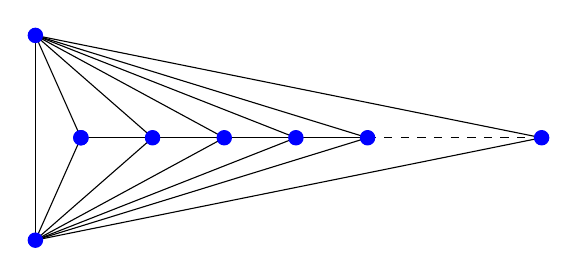
\begin{tikzpicture}[rotate=90, scale=1.3]

\coordinate (U) at (0.553380,1.150606);
\coordinate (V) at (2.553380,1.150606);
\coordinate (W) at (1.553380,0.70606);

\coordinate (W1) at ($(W) + 0*(0,-0.7)$);
\coordinate (W2) at ($(W) + 1*(0,-0.7)$);
\coordinate (W3) at ($(W) + 2*(0,-0.7)$);
\coordinate (W4) at ($(W) + 3*(0,-0.7)$);
\coordinate (W5) at ($(W) + 4*(0,-0.7)$);
\coordinate (W6) at ($(W) + 5*(0,-0.9)$);

\draw (U) -- (V);
\draw (U) -- (W);
\draw (V) -- (W);

\draw (W1) -- (W2);
\draw (U) -- (W2);
\draw (V) -- (W2);

\draw (W2) -- (W3);
\draw (U) -- (W3);
\draw (V) -- (W3);

\draw (W3) -- (W4);
\draw (U) -- (W4);
\draw (V) -- (W4);

\draw (W4) -- (W5);
\draw (U) -- (W5);
\draw (V) -- (W5);

\draw [dashed] (W5) -- (W6);
\draw (U) -- (W6);
\draw (V) -- (W6);

\filldraw[blue] (U) circle (0.07cm);
\filldraw[blue] (V) circle (0.07cm);
\filldraw[blue] (W) circle (0.07cm);
\filldraw[blue] (W1) circle (0.07cm);
\filldraw[blue] (W2) circle (0.07cm);
\filldraw[blue] (W3) circle (0.07cm);
\filldraw[blue] (W4) circle (0.07cm);
\filldraw[blue] (W5) circle (0.07cm);
\filldraw[blue] (W6) circle (0.07cm);

\end{tikzpicture}}
}
\endgroup
\end{center}
\caption{The graph $P_2 + P_{n-2}$.
   \label{fig-pn4}}
\end{figure}


\begin{lemma}\label{planar trivial spectral bound}
$\sqrt{6n} > \lambda_1> \sqrt{2n-4}$.
\end{lemma}
\begin{proof}
For the lower bound, first note that the graph $K_{2,n-2}$ is planar and is a strict subgraph of some other planar graphs on the same vertex set. Since $G$ has maximum spectral radius among all planar graphs on $n$ vertices,
\[
 \lambda_1 > \lambda_1(K_{2,n-2}) = \sqrt{2n-4}.
 \]
 For the upper bound, since the sum of the squares of the eigenvalues equals twice the number of edges in $G$, which is
 at most $6n-12$ by planarity, we get that $\lambda_1 < \sqrt{6n-12} < \sqrt{6n}$.
\end{proof}

%We never use all of this averaging right? TK
%By the eigenvector equation, we see
%\[
%\lambda^2 = \sum_{y\sim x}\sum_{z\sim y} z \leq \sum_{uv\in E(G)} (u+v) - \sum_{y\sim x} y = \sum_{uv\in E(G)} (u+v) - \lambda.
%\]
%Rearranging and dividing by $2|E(G)|$ we have
%\[
%\frac{1}{2m} (\lambda^2+\lambda) \leq \frac{1}{2m} \sum_{uv\in E(G)} u+v.
%\]
%Because $G$ is planar, $m\leq 2n-6$, and so we have that the average over all $uv\in E(G)$ of the quantity $\frac{u+v}{2}$ is 
%\begin{equation}\label{average edge one third}
%\mathrm{avg}_{uv\in E(G)} \frac{u+v}{2} \geq \frac{2n-4 + \sqrt{2n-4}}{6n-12} > \frac{1}{3}.
%\end{equation}

Next we partition the graph into vertices of small eigenvector entry and those with large eigenvector entry.  Fix $\epsilon > 0$,
whose exact value will be chosen later.  Let 
\[
L:= \{z\in V(G): z> \epsilon\}
\]
and $S = V(G) \setminus L$. For any vertex $z$, the eigenvector equation gives $z\sqrt{2n-4} < z\lambda_1\leq d_z$. Therefore,
\[
2(3n - 6)  \geq \sum_{z\in V(G)} d_z \geq \sum_{z\in L} d_z \geq |L|\epsilon \sqrt{2n-4},
\]
yielding $|L| \leq \frac{3\sqrt{2n-4}}{\epsilon}$. Since the subgraph of $G$ consisting of edges with one endpoint in $L$ and one endpoint in $S$ is a bipartite planar graph, we have $e(S,L) \leq 2n-4$, and since the subgraphs induced by $S$ and by $L$ are each planar, we have $e(S) \leq 3n-6$ and $e(L) \leq \frac{9\sqrt{2n-4}}{\epsilon}$. 

%Similarly to before
%\[
%\lambda^2 + \lambda_1\leq \sum_{uv\in E(G)} u+v = \sum_{uv\in E(S,L)} u+v + \sum_{uv\in E(S)} u+v + \sum_{uv\in E(L)} u+v \leq \sum_{uv\in E(S,L)} (u+v )+ 6\epsilon n + \frac{18\sqrt{n}}{\epsilon}.
%\]
%Dividing both sides by $2e(S,L)$, we have that for $n$ large enough
%\[
%\frac{(2-7\epsilon)n}{2e(S,L)} \leq \frac{1}{e(S,L)}\sum_{uv\in E(S,L)} \frac{u+v}{2}.
%\]
%Since $e(S,L) \leq 2n-4$, we have that the average over $uv\in E(S,L)$ of the quantity $\frac{u+v}{2}$ satisfies 
%\begin{equation}\label{average bipartite edge one half}
%\mathrm{avg}_{uv\in E(S,L)} \frac{u+v}{2} > \frac{1}{2} - 2\epsilon.
%\end{equation}

Next we show that there are two vertices adjacent to most of $S$. The first step towards this is an upper bound on the sum of eigenvector entries in both $L$ and $S$.
\begin{lemma}
\begin{equation}\label{eigenvector norm L}
\sum_{z\in L} z \leq  \epsilon \sqrt{2n-4} + \frac{18}{\epsilon}
\end{equation}
\noindent and
 \begin{equation}\label{eigenvector norm S}
 \sum_{z\in S} z \leq (1+3\epsilon)\sqrt{2n-4}
 \end{equation}

\end{lemma}
\begin{proof}
\[
\sum_{z\in L} \lambda_1z = \sum_{z\in L} \sum_{y\sim z} y = \sum_{z\in L}\left( \sum_{\substack{y\sim z \\ y\in S}} y + \sum_{\substack{y\sim z\\ y\in L}} y \right) \leq \epsilon e(S,L) + 2e(L) \leq \epsilon (2n-4) + \frac{18\sqrt{2n-4}}{\epsilon}.
\]
Dividing both sides by $\lambda_1$ and using Lemma \ref{planar trivial spectral bound} gives \eqref{eigenvector norm L}.

 On the other hand,
 \[
 \sum_{z\in S} \lambda_1z = \sum_{z\in S}\sum_{y\sim z} y \leq 2\epsilon e(S) + e(S,L) \leq (6n-12)\epsilon  + (2n-4).
 \]
 Dividing both sides by $\lambda_1$ and using Lemma \ref{planar trivial spectral bound} gives \eqref{eigenvector norm S}.
 \end{proof}

 Now let $u\in L$
\[
u\sqrt{2n-4} \leq \lambda_1u=\sum_{y\sim u} y = \sum_{\substack{y\sim u \\ y\in L}} y + \sum_{\substack{y\sim u\\ y\in S}} y \leq \sum_{y\in L} y + \sum_{\substack{y\sim u \\y\in S}} y.
\]
By \eqref{eigenvector norm L}, this gives
\begin{equation}\label{eigenvector norm neighbors of w}
\sum_{\substack{y\sim u \\ y\in S}} y \geq (u-\epsilon)\sqrt{2n-4} - \frac{18}{\epsilon}.
\end{equation}

 
 The equations \eqref{eigenvector norm S} and \eqref{eigenvector norm neighbors of w} imply that if $u\in L$ and $u$ is close to $1$, then the sum of the eigenvector entries of vertices in $S$ not adjacent to $u$ is small. To conclude that this implies $u$ is adjacent to most vertices in $S$ we need the following lemma.
 
\begin{lemma}\label{eigenvector entry lower bound}
For all $z$ we have $z>\frac{1}{\sqrt{6n}}$.
\end{lemma}
\begin{proof}
  By way of contradiction assume $z\leq \frac{1}{\sqrt{6n}} < \frac{1}{\lambda_1}$. By the eigenvector equation $z$ cannot be adjacent to $x$, since
  $x$ has eigenvector entry $1$. Let $H$ be the graph obtained from $G$ by removing all edges incident with $z$ and making $z$ adjacent to $x$. By the Rayleigh quotient, we have $\lambda_1(H) > \lambda_1(G)$, a contradiction.
\end{proof}

\noindent Now letting $u=x$ and combining \eqref{eigenvector norm neighbors of w} and \eqref{eigenvector norm S} gives 
\[
(1+3\epsilon)\sqrt{2n-4} \geq \sum_{\substack{y\in S\\ y\not\sim x}} y + \sum_{\substack{y\in S\\ y\sim x}} y \geq \sum_{\substack{y\in S\\ y\not\sim x}} y + (1-\epsilon)\sqrt{2n-4} - \frac{18}{\epsilon}.
\]
Now applying Lemma \ref{eigenvector entry lower bound} gives
\[
|\{y\in S: y\not\sim x\}| \frac{1}{\sqrt{6n} }\leq 4\epsilon \sqrt{2n-4} + \frac{18}{\epsilon}.
\]
For $n$ large enough, we have $|\{y\in S: y\not\sim x\}| \leq 14\epsilon n$. So $x$ is adjacent to most of $S$. Our next goal is to show that there is another vertex in $L$ that is adjacent to most of $S$.

\begin{lemma}\label{second vertex of large degree}
There is a $w\in L$ with $w\not=x$ such that $w> 1-24\epsilon$ and $|\{y\in S: y\not\sim w\}| \leq 94\epsilon n$.
\end{lemma}
\begin{proof}
By the eigenvector equation, we see
\[
\lambda_1^2 = \sum_{y\sim x}\sum_{z\sim y} z \leq \left(\sum_{uv\in E(G)} u+v\right) - \sum_{y\sim x} y = \left(\sum_{uv\in E(G)} u+v\right) - \lambda_1.
\]
Rearranging and noting that $e(S) \leq 3n-6$ and $e(L) \leq \frac{9\sqrt{2n-4}}{\epsilon}$ since $S$ and $L$ both induce planar subgraphs gives
\begin{align*}
& 2n-4\leq \lambda_1^2 + \lambda_1\leq \sum_{uv\in E(G)} u+v = \left(\sum_{uv\in E(S,L)} u+v\right) + \left(\sum_{uv\in E(S)} u+v\right) + \left(\sum_{uv\in E(L)} u+v \right) \\
& \leq \left(\sum_{uv\in E(S,L)} u+v \right) + \epsilon(6n-12) + \frac{18\sqrt{2n-4}}{\epsilon}.
\end{align*}
So for $n$ large enough,
\[
(2-7\epsilon)n \leq \sum_{uv\in E(S,L)} u+v =\left( \sum_{\substack{uv\in E(S,L)\\ u=x}} u+v\right) + \left(\sum_{\substack{uv\in E(S,L)\\ u\not= x}} u+v\right) \leq \epsilon e(S,L) + d_x + \sum_{\substack{uv\in E(S,L)\\ u\not= x} } u
\]
giving
\[
\sum_{\substack{uv\in E(S,L)\\ u\not = x}} u \geq (1-9\epsilon)n.
\]

Now since $d_x \geq |S| - 14\epsilon n > (1-15\epsilon)n$, and $e(S,L) < 2n$, the number of terms in the left hand side of the sum is at most $(1+15\epsilon)n$. By averaging, there is a $w\in L$ such that 
\[
w \geq \frac{1-9\epsilon}{1+15\epsilon} > 1-24\epsilon,
\]
for $\epsilon$ small enough. Applying \eqref{eigenvector norm neighbors of w} and \eqref{eigenvector norm S} to this $w$ gives
\[
(1+3\epsilon) \sqrt{2n-4} \geq \sum_{\substack{y\in S\\ y\not\sim w}} y + \sum_{\substack{y\in S\\ y\sim w}} y \geq \sum_{\substack{y\in S\\ y\not\sim w}} y + (1-21\epsilon)\sqrt{2n-4} + \frac{18}{\epsilon},
\]
and applying Lemma \ref{eigenvector entry lower bound} gives that for $n$ large enough
\[
|\{y\in S: y\not\sim w\}| \leq 94\epsilon n
\]
for $n$ large enough.

\end{proof}
\medskip

For the rest of the section, let $w$ be the vertex from Lemma \ref{second vertex of large degree}. So $x=1$ and $w> 1-24\epsilon$, and both are adjacent to most of $S$. Our next goal is to show that all of the remaining vertices are adjacent to both $x$ and $w$. Let $B = N(x) \cap N(w)$ and $A = V(G) \setminus \{x\cup w \cup B\}$. We show that $A$ is empty in two steps: first we show the eigenvector entries of vertices in $A$ are as small as we need, which we then use to show that if there is a vertex in $A$ then $G$ is not extremal.

\begin{lemma}\label{eigenvector entries of A small}
Let $v\in V(G) \setminus \left\{ x,w \right\}$. Then $v < \frac{1}{10}$.
\end{lemma}

\begin{proof}
We first show that the sum over all eigenvector entries in $A$ is small, and then we show that each eigenvector entry is small. Note that for each $v\in A$, $v$ is adjacent to at most one of $x$ and $w$, and is adjacent to at most $2$ vertices in $B$ (otherwise $G$ would contain a $K_{3,3}$ and would not be planar). Thus
\[
\lambda_1\sum_{v\in A} v \leq \sum_{v\in A} d_v \leq 3|A| +2e(A) < 9|A|,
\]
where the last inequality is using that $e(A) < 3|A|$ since $A$ induces a planar graph. Now, since $|L| < \frac{3\sqrt{2n-4}}{\epsilon} < 1\epsilon n$ for $n$ large enough, we have $|A| \leq (14+94+1)\epsilon n$ (by Lemma \ref{second vertex of large degree}) . Therefore 
\[
\sum_{v\in A} v \leq \frac{9\cdot 109 \cdot \epsilon n}{\sqrt{2n-4}}.
\]

Now any $v\in V(G) \setminus \left\{ x,w \right\}$ is adjacent to at most 4 vertices in $B \cup \left\{x,w \right\}$, as otherwise we would have a $K_{3,3}$
as above.  So we get
\[
\lambda_1v = \sum_{u\sim v} u \leq 4 + \sum_{\substack{u\sim v\\ u\in A}} u \leq 4 + \sum_{u\in A} u \leq C\epsilon\sqrt{n}
\]
where $C$ is an absolute constant not depending on $\epsilon$. Dividing both sides by $\lambda_1$ and choosing $\epsilon$ small enough yields the result.
\end{proof}

We use the fact that the eigenvector entries in $A$ are small to show that if $v\in A$ (ie $v$ is not adjacent to both $x$ and $w$), then removing all edges from $v$ and adding edges from it to $x$ and $w$ increases the spectral radius, showing that $A$ must be empty. To do this, we must be able to add edges from a vertex to both $x$ and $w$ and have the resulting graph remain planar. This is accomplished by the following lemma.

\begin{lemma}\label{x connected to w}
If $G$ is extremal, then $x\sim w$.
\end{lemma}

Once $x\sim w$, one may add a new vertex adjacent to only $x$ and $w$ and the resulting graph remains planar.

\begin{proof}[Proof of Lemma \ref{x connected to w}]
From above, we know that for any $\delta > 0$, we may choose $\epsilon$ small enough so that when $n$ is sufficiently
large we have $d_x > (1-\delta)n$ and $d_w > (1-\delta)n$.  By maximality
of $G$, we also know that $G$ has precisely $3n-6$ edges, and by Euler's formula, any planar drawing of $G$ has $2n-4$ faces, each of which is bordered by precisely three edges of $G$ (because in a maximal planar graph, every face is a triangle).    


Now we obtain a bound on the number of faces that $x$ and $w$ must be incident to.  Let $X$ be the set of edges incident to $x$.  Each edge in $G$ is incident to precisely two faces, and each face can be incident to at most two edges in $X$ (again, since each face is a triangle by maximality).  So $x$ is incident to at least $|X| = d_x \geq (1-\delta)n$ faces.  Similarly, $w$ is incident to at least $(1-\delta)n$ faces. 


Let $F_1$ be the set of faces that are incident to $x$, and then let $F_2$ be the set of faces that are not incident to $x$, but which share an edge with a face in $F_1$.  Let $F = F_1 \cup F_2$.  We have that $|F_1| \geq (1-\delta)n$.  Now each
face in $F_1$ shares an edge with exactly three other faces:  if two faces shared two edges, then since each face is a triangle
both faces must be bounded by the same three edges;  this cannot happen, except in the degenerate case when $n=3$.  At most two of these three faces are in $F_1$, and so $|F_2| \geq |F_1| / 3 \geq (1-\delta)n / 3$.  Hence, $|F| \geq (1-\delta)4n / 3$, and so the sum of the number of faces
in $F$ and the number of faces incident to  $w$ is larger than $2n-4$.  In 
particular, there must be some face $f$ that is both belongs to $F$ and is incident to $w$.


Since $f \in F$, then either $f$ is incident to $x$ or $f$ shares an edge with some face that is incident to $x$.  If $f$ is incident to both $x$ and $w$, then $x$ is adjacent to $w$ and 
we are done.  Otherwise, $f$ shares an edge $\left\{y,z\right\}$ with a face $f'$ that is incident to $x$.  In this case, deleting the edge $\left\{y,z\right\}$ and inserting the edge $\left\{x,w\right\}$ yields a planar graph $G'$.  By lemma~\ref{eigenvector entries of A small}, 
the product of the eigenvector entries of $y$ and $z$ is less than $1/100$,
which is smaller than the product of the eigenvector entries of $x$ and $w$.  
This implies that $\lambda_1(G') > \lambda_1(G)$, which is a contradiction.
\end{proof}

We now show that every vertex besides $x$ and $w$ is adjacent to both $x$ and $w$.

\begin{lemma}\label{A empty}
$A$ is empty.
\end{lemma}

\begin{proof}
By way of contradiction, assume $A$ is nonempty. $A$ induces a planar graph, therefore if $A$ is nonempty, then there is a $v\in A$ such that $|N(v)\cap A| < 6$. Further, $v$ has at most $2$ neighbors in $B$ (otherwise $G$ would contain a $K_{3,3}$. Recall that $\textbf{v}$ is the principal eigenvector for the adjacency matrix of $G$. Let $H$ be the graph with vertex set $V(G) \cup \{v'\} \setminus \{v\}$ and edge set $E(H) = E(G\setminus\{v\}) \cup \{v'x, v'w\}$. By Lemma \ref{x connected to w}, $H$ is a planar graph. Then 
\begin{align*}
\textbf{v}^T \textbf{v}\lambda_1(H) &\geq \textbf{v}^T A(H) \textbf{v} & \\
& = \textbf{v}^T A(G) \textbf{v} - 2\sum_{z\sim v} vz + 2v(w+x) & \\
& \geq \textbf{v}^T A(G) \textbf{v} - 14\cdot v \cdot \frac{1}{10} - 2\sum_{\substack{z\sim v\\ z\in \{w,x\}}} vz + 2v(w+x) & \mbox{(by Lemma \ref{eigenvector entries of A small})} \\
& \geq \textbf{v}^T A(G) \textbf{v} - \frac{14}{10}v + 2vw & \mbox{($|N(v)\cap \{x,w\}| \leq 1$)} \\
& > \textbf{v}^T A(G) \textbf{v} & \mbox{(as $w>7/10$)}\\
&= \textbf{v}^T\textbf{v} \lambda_1(G).
\end{align*}
So $\lambda_1(H) > \lambda_1(G)$ and $H$ is planar, ie $G$ is not extremal, a contradiction.
\end{proof}


We now have that if $G$ is extremal, then $K_2+I_{n-2}$, an edge joined to an independent set of size $n-2$, is a subgraph of $G$. Finishing the proof is straightforward.

\subsection{Proof of Main Theorem}

\begin{theorem}
For $n\geq N_0$, the unique planar graph on $n$ vertices with maximum spectral radius is $K_{2} + P_{n-2}$.
\end{theorem}

\begin{proof}
By Lemmas \ref{x connected to w} and \ref{A empty}, we have that $x$ and $w$ have degree $n-1$. We now look at the set $B = V(G) \setminus \{x,w\}$. For $v\in B$, we have $|N(v) \cap B| \leq 2$, otherwise $G$ contains a copy of $K_{3,3}$. Therefore, the graph induced by $B$ is a disjoint union of paths, cycles, and isolated vertices. However, if there is some cycle $C$ in the graph induced by $B$, then $C \cup\{x,w\}$ is a subdivision of $K_5$. So the graph induced by $B$ is a disjoint union of paths and isolated vertices. However, if $B$ does not induce a path on $n-2$ vertices, then $G$ is a strict subgraph of $K_2 + P_{n-2}$, and we would have $\lambda_1(G) < \lambda_1(K_2 + P_{n-2})$. Since $G$ is extremal, $B$ must induce $P_{n-2}$ and so $G = K_2 + P_{n-2}$.
\end{proof}

This chapter is based on part of the paper ``Three conjectures in extremal spectral graph theory'',
 \cite{TaitTobin2017}, to appear in \textit{Journal of Combinatorial Theory, Series B},
written jointly with Michael Tait.  The dissertation
author was the primary investigator and author of the paper.

%%%%%%%%%%%%%%%%%%%%%%%%%%%%%%%%%%%%%%%%%%%%%%%%%%%%%%%%%%%%%%%%%%%%%%%%%%
%% SECTION ONE
%%%%%%%%%%%%%%%%%%%%%%%%%%%%%%%%%%%%%%%%%%%%%%%%%%%%%%%%%%%%%%%%%%%%%%%%%%

\chapter{The Spectral Gap of Reversal Graphs}

\section{Introduction}


Consider a permutation $\tau$ in the symmetric group $S_n$, written in 
word notation $(\tau_1, \tau_2, \cdots, \tau_n)$, where we denote $\tau(i) = \tau_i$.  
A \textit{substring} is a subsequence of $\tau$, $(\tau_i, \tau_{i+1}, \ldots, \tau_j)$,
for some $1 \leq i < j\leq n$, and \textit{reversing} this substring yields
$(\tau_j, \tau_{j-1}, \ldots, \tau_i)$.
A \textit{substring reversal} of $\tau$ is any permutation obtained from $\tau$
by reversing a substring in $\tau$. 
Substring reversal is a well-studied operation on permutations, and 
often  appears in metrics on permutations, edit distances
and permutation statistics. There are numerous applications involving many variations of substring reversal,
such as genome arrangements and sequencing  (see \cite{BafnaPevzner1996}, \cite{Hannenhalli1996}, \cite{KececiogluSankoff1995}). 

The \textit{reversal graph} $R_n$ is the graph whose vertex set is the permutation group $S_n$, where
two vertices are adjacent if they are substring reversals of each other. Thus, $R_n$ has $n!$ vertices and is regular
with degree
$\binom {n} 2$.
Many properties of  the reversal graph $R_n$ have long been studied.
One interesting problem is to determine the minimum number of substring reversals needed to transform one
given permutation in $S_n$ to another, which is equivalent to finding 
a shortest path in $R_n$.  The smallest number of reversals required to turn any permutation into any other
is exactly the diameter of $R_n$, and 
it was shown in \cite{BafnaPevzner1996} that the diameter of 
the reversal graph is exactly $n-1$. The connectivity
and hamiltonicity of $R_n$ were investigated in \cite{LiMeng2008}. 
There are  still many questions concerning $R_n$ that remain unresolved. In this section, we examine
 the eigenvalues of  $R_n$, and determine the second largest eigenvalue of the adjacency matrix of $R_n$.
 Note that the second largest adjacency eigenvalue of a regular graph is intimately related to the
 rate of convergence for random walks on a graph. We use methods from graph coverings to determine
 the second largest eigenvalue of $R_n$, although our techniques cannot be used to determine
 the whole spectrum of $R_n$.



 An intriguing variation of substring reversal is  {\it prefix reversal} (or {\it pancake flipping}) where only
 substrings of the form $(\tau_1, \ldots, \tau_j)$ are allowed to be reversed.
The \textit{prefix reversal graph}, or  the \textit{pancake graph}, $\mathcal{P}_n$ 
is a special subgraph of $R_n$.  ${\mathcal P}_n$  also has vertex set $S_n$  but
the edge set is  restricted. In $\mathcal{P}_n$, the 
neighbors of $\tau$ are the permutations of the form  
 \[ (\tau_k, \tau_{k-1}, \cdots, \tau_1, \tau_{k+1}, \cdots, \tau_n) \]
for $1 < k \leq n$.
 In contrast to the reversal graph
where the exact value of the diameter is known, the problem of determining the diameter of the pancake  
graph has a long history and still remains open.
This problem was first posed by Jacob Goodman, under the pseudonym Harry Dweighter, as a Monthly problem
in 1975 \cite{Dweighter1975}.
The current best upper bound is $f(n) \leq \frac{18}{11} n $, due to
Chitturi et al. \cite{ChitturiEtAl2009}, improving on a previous bound of $\frac{5}{3} n$ given by
 Gates and Papadimitriou \cite{GatesPapadimitriou1979} in 1979.  The best lower bound is
$f(n) \geq 15 \left\lfloor \frac{n}{14} \right\rceil$, which is due to 
Heydari and Sudborough \cite{HeydariSudborough1997}.  Recently it was shown that the problem of  determining the exact minimum number of flips
to transform  one permutation $\tau_1$ into another permutation $\tau_2$, for two
given permutations $\tau_1$ and $\tau_2$, is NP--hard \cite{BulteauEtAl2015}.
  In \cite{Cesi2009}, it 
was determined that the spectral gap of $\mathcal{P}_n$ is one, answering a 
question posed in \cite{GunnellsEtAl2007}.
We will determine the spectral gaps for a family of graphs which contains certain Cayley graphs
including $\mathcal{P}_n$, giving an alternative proof in that case.
We then use the spectral gap of $\mathcal{P}_n$, together with a decomposition of $R_n$
into $P_n$ and copies of $R_{n-1}$, to determine the second largest
eigenvalue of $R_n$.


\begin{theorem}\label{thm:rev_eig}
 If $\lambda_1,\lambda_2$ are the two largest eigenvalues of the adjacency matrix
 of $R_n$, then  
 \[  \lambda_1 = \binom{n}{2}, \text{ and } \lambda_2 = \binom{n}{2}-n. \]
\end{theorem}



We will consider a family of graphs that generalizes the pancake graph, 
and show that for every graph in this family the spectral gap is one. 

\begin{theorem}\label{thm:main}
 Let $\mathcal{F}_n$ be the set of all graphs whose vertex set is the symmetric
 group $S_n$, and where for each vertex $\tau$ and each $2 \leq i \leq n$, 
 $\tau$ is adjacent to exactly one vertex of the form 
 \[ (\tau_i, \alpha_2, \alpha_3, \cdots, \alpha_{i-1}, \tau_1, \tau_{i+1}, \cdots, \tau_n). \]
 That is, the first and $i$th entries are swapped, and the entries in between are possibly rearranged.
 Then for any graph $G \in \mathcal{F}_n$, the two largest eigenvalues of
 the adjacency matrix of $G$ are $n-1$ and $n-2$.  In particular, the 
 adjacency spectral gap of $G$ is $1$.
\end{theorem}

The graphs $R_n$ and $\mathcal{P}_n$, as well as many of the graphs in 
$\mathcal{F}_n$, are Cayley graphs of the symmetric group $S_n$.
Indeed, Cayley graphs of the symmetric group  
have been the subject of extensive study,
with particular interest in their spectral gap.  In \cite{Lubotzky1995}, 
Lubotzky posed the problem of finding a family of $k$-regular Cayley
graphs of $S_n$ with spectral gap bounded away from zero;  an explicit
construction of such a family was found in \cite{Kassabov2007}.  For many 
particular Cayley graphs of $S_n$, the spectral gap has been computed
\cite{Friedman2000,FlattoEtAl1985,Cesi2009},
and the case when $S$ consists of transpositions is particularly well-studied.
Of particular relevance here, the Cayley graph with generating set
\[S = \{(1\ k) : 2 \leq k \leq n\}\] 
belongs to the family $\mathcal{F}_n$, and
the spectral gap was determined to be $1$ in \cite{FlattoEtAl1985}.


The remainder of the paper is organized as follows.  In Section 2 we review
the necessary background and establish notation.  In Section 3 we recall
the notions of graph coverings and projections, which we will use frequently 
in our proofs.  In Section 4 we introduce a graph which is a projection
of every graph in the family $\mathcal{F}_n$, which provides a lower bound of one
on the spectral gap of every graph in this family.  We establish the corresponding upper bound in Section 5.
In Section 6 we prove Theorem~\ref{thm:rev_eig} and further investigate
the spectrum of $R_n$.  We conclude with some problems and remarks.



%%%%%%%%%%%%%%%%%%%%%%%%%%%%%%%%%%%%%%%%%%%%%%%%%%%%%%%%%%%%%%%%%%%%%%%%%%
%% SECTION TWO
%%%%%%%%%%%%%%%%%%%%%%%%%%%%%%%%%%%%%%%%%%%%%%%%%%%%%%%%%%%%%%%%%%%%%%%%%%

%\section{Preliminaries}
Before proceeding to define the graph spectra of interest here, we note that
the definitions of eigenvalues and eigenvectors are much simpler and cleaner for regular graphs
than those of weighted irregular graphs. Although the graphs 
$R_n$ and the graphs in $\mathcal{F}_n$, are regular, we will consider various
associated graphs which are irregular and weighted in order to determine the spectral
gap that we need.
Furthermore, we remark that the spectral gap of the adjacency matrix of a weighted or unweighted graph often depends
on a few of the largest degrees and therefore the spectral gap of the adjacency matrix  can {\it  not}
be used to determine the rate of convergence for random walks on irregular graphs.  Instead it is more appropriate
to study the combinatorial Laplacian and normalized Laplacian.
In this section, we consider general weighted graphs and define the eigenvalues of the normalized Laplacian,
which will be important when we define graph covers.
For undefined terminology, the reader is referred to  \cite{Chung1997}.


%We will use the following standard result from matrix analysis, see for 
%example \cite{HornJohnson}.  
%\begin{theorem}[Rayleigh--Ritz]\label{rayleigh}
%If $M$ is a Hermitian matrix, then the $k$th largest eigenvalue satisfies
% \[ \lambda_k(M) = \max_{\textbf{v} \perp V_{k-1}} \frac{\textbf{v}^t M \textbf{v}}{\textbf{v}^t \textbf{v}}\]
%where $V_{k-1}$ is the vector space generated by $k-1$ eigenvectors 
%corresponding to the largest $k-1$ eigenvalues, and $V_0 = \emptyset$.
%\end{theorem}


Let $G$ denote a weighted undirected graph with edge weight $w_{u,v} = w_{v,u}$. The adjacency matrix
of $G$, denoted by $A_G$, has entries $A_G(u,v)= w_{u,v}$ for vertices $u$ and $v$.  For any
vertex $v \in V(G)$, the set of vertices adjacent to $v$ is denoted by $N(v)$.
The degree $d_v$ of a vertex $v$ is defined to be
\[ d_v = \sum_u w_{u,v}. \]
We will only consider weighted graphs without isolated vertices, i.e., $d_v > 0$ for all $v$.
Let $D_G$ be the diagonal 
degree matrix whose $i$th diagonal entry is equal to the degree of the $i$th
vertex.  Then the combinatorial Laplacian of $G$ is $L_G = D_G - A_G$, 
and the normalized Laplacian is $\mathcal{L}_G = D_G^{-1/2} L_G D_G^{-1/2}$.
For a $d$-regular graph, we have $\mathcal{L}_G =1 - \frac{1}{d} A_G$.
The eigenvalues of the normalized Laplacian $\mathcal{L}_G$ are denoted by
$0=\mu_0 \leq \mu_1 \leq \ldots \leq \mu_{n-1}$ where $n$ is the number of vertices in $G$.
$\mu_1$ is called the spectral gap of the normalized Laplacian, and the rate of convergence of random walks on $G$ 
with transition probability matrix $P=D_G^{-1} A_G$ is exactly $\mu_1^{-1}$ (see \cite{Chung1997}).  We will denote the eigenvalues of 
the adjacency matrix of $G$ by $\lambda_1 \geq \lambda_2 \geq \cdots \geq \lambda_n$,
and $\lambda_1 - \lambda_2$ is the spectral gap of the adjacency matrix. For a regular graph of degree $d$, $\lambda_1=d$
and $\lambda_2 = d (1-\mu_1)$.

Let $\phi_i$ denote the orthonormal eigenvector associated with $\mu_i$.  It can easily be shown that
$\phi_0 = D_G^{1/2}/\sqrt{\vol(G)}$ where $\vol(G)=\sum_v d_v$.
%From the
%Rayleigh--Ritz Theorem, we have
%\begin{align*}
%\mu_1&= \inf_{g \perp \phi_0} \frac{ \langle g, \mathcal{L}_G g \rangle}{\langle g, g \rangle}\\
%&= \inf_{f \perp D_G \mathbf{1}}  \frac{ \langle f, {L}_G f \rangle}{\langle f, D_G f \rangle}\\
%&= \inf_{f \perp D_G \mathbf{1}} \frac{\sum_{x \sim y} (f(x)-f(y))^2w_{x,y}}{\sum_x f^2(x) d_x}
%\end{align*} 
Instead of dealing with eigenvectors $\phi_i$ of $\mathcal{L}_G$, it is often convenient to consider
the corresponding
\textit{harmonic eigenfunction} defined by $f_i = D_G^{-1/2} \phi_i$ which satisfies
\[  \mu_i f_i(u)d_u= \sum_{v} w_{u,v} (f(u)-f(v))  \]
for all vertices $u$.  Note that for regular graphs, 
harmonic eigenfunctions are exactly eigenfunctions.
Moreover, for regular graphs the eigenfunctions of $\mathcal{L}, L$
and $A$ are the same, and the corresponding spectra are translations of each other.




We will frequently deal with permutations, so we establish
the notation that we will use.  The symmetric group is denoted as $S_n$
throughout.  Every permutation will be given in \textit{word notation}, 
that is, as a list of numbers $(\tau_1, \tau_2, \cdots, \tau_n)$, which indicates
that permutation $\tau$ maps $i$ to $\tau_i$.  We will sometimes refer to the 
value $\tau_i$ as the $i$th \textit{entry} or \textit{position} of the permutation $\tau$.
When we write the product
of two permutations, such as $\pi \sigma$, we take this to mean: first apply
permutation $\sigma$, then apply permutation $\pi$.


As discussed in Section~1, $R_n$ and many of the graphs in 
the family $\mathcal{F}_n$ are Cayley
graphs.  We briefly recall the definition here.  Let $H$ be a finite group, and 
$S$ a subset of $H$.  We say that $S$ is a symmetric set if whenever $s \in S$, 
we also have $s^{-1} \in S$.  Given a symmetric set $S$ that generates the 
group $H$, the right-Cayley graph $\text{Cay}_R(H,S)$ is the graph with vertex set
equal to $H$, and edges of the form $\{x, xs\}$ for all $x \in H, s \in S$.
This is an undirected $|S|$-regular graph. A left-Cayley graph is defined similarly,
with edges of the form $\{x,sx\}$.  For example, let $S$ be the set of
permutations corresponding to substring reversals.  That is, $S$ consists of 
the 
permutations obtained from taking the identity permutation 
$(1, 2, 3, \cdots, n)$ and reversing a substring.  Then 
$R_n = \text{Cay}_R(S_n,S)$.

%%%%%%%%%%%%%%%%%%%%%%%%%%%%%%%%%%%%%%%%%%%%%%%%%%%%%%%%%%%%%%%%%%%%%%%%%%
%% SECTION THREE
%%%%%%%%%%%%%%%%%%%%%%%%%%%%%%%%%%%%%%%%%%%%%%%%%%%%%%%%%%%%%%%%%%%%%%%%%%

%\section{Graph coverings}
In proving Theorem~\ref{thm:main} and Theorem~\ref{thm:rev_eig}, we will rely heavily on graph coverings, an idea developed in \cite{ChungYau1998}.  A short overview is presented here.  Let $G$ and $ \tilde{G}$ be two weighted graphs.  Then $\tilde{G}$ is a \textit{covering} of $G$ if there is a surjection $\pi : V(\tilde{G}) \to V(G)$ satisfying the following two properties:
\begin{itemize}
 \item[(1)] For $x,y \in V(\tilde{G})$, where $\pi(x) = \pi(y)$, and for any $v \in V(G)$
 \[ \displaystyle \sum_{z \in \pi^{-1}(v)} w(z,x) = \displaystyle \sum_{z \in \pi^{-1}(v)} w(z,y) . \]
 \item[(2)] There is a fixed $m \in \mathbb{R}^{+} \cup \{\infty\}$, the \textit{index} of $\pi$, such that for all $u,v \in V(G)$
 \begin{equation}\label{covering_sum_condition}
  \displaystyle \sum_{\substack{x \in \pi^{-1}(u) \\ y \in \pi^{-1}(v)}} w(x,y) = m w(u,v) .
 \end{equation}
\end{itemize}
As $\pi$ is a surjection, it can alternatively be viewed as a partition of the vertices of $V(\tilde{G})$ into $|V(G)|$ sets.  With this interpretation, the above definition can be seen as a generalization of an \textit{equitable partition}; see, for example, \cite{GodsilRoyle2013}.
We say that $G$ is a {\it projection} of $\tilde{G}$ via the mapping $\pi$ if $\tilde{G}$ is a covering of $G$ under $\pi$.


The virtue of a graph covering is that there is a strong correspondence between the eigenvalues of a covering graph and the eigenvalues of the projection.  This correspondence is the content of the following theorem, which is proved in \cite{ChungYau1998}.

\begin{theorem}\label{thm:cov-cor}
\emph{(Covering-Correspondence)} \\
Let $G, \tilde{G}$ be two weighted undirected graphs, and $\pi : V(\tilde{G}) \to V(G)$ be a covering map.  For any function $f : V(\tilde{G}) \to \mathbb{C}$, define $p_f : V(G) \to \mathbb{C}$ by
 \[ p_f(v) = \displaystyle \sum_{x \in \pi^{-1}(v)} \frac{f(x) d_x}{d_v} . \]
For any function $f : V(G) \to \mathbb{C}$, define the \textit{lift} of $f$, $l_f : V(\tilde{G}) \to \mathbb{C}$ by
 \[ l_f(x) = f(u), \text{ where $\pi(x) = u$}. \]
  
\begin{itemize}
 \item[(i)]  If $\mu$ is an eigenvalue of $G$ with harmonic eigenfunction $f$, then $\mu$ is an eigenvalue of $\tilde{G}$ with harmonic eigenfunction $l_f$.
 \item[(ii)] If $\mu$ is an eigenvalue of $\tilde{G}$ with harmonic eigenfunction $f$, then if $p_f \neq 0$, $\mu$ is an eigenvalue of $G$ with harmonic eigenfunction $p_f$.
\end{itemize}
\end{theorem}

We will use this theorem in the form of the following corollary.

\begin{corollary}\label{cor:cov-cor}
  Let $G$ be a graph with cover $\tilde{G}$, under covering map $\pi$,
  where $\tilde{G}$ is a regular graph.  Then the eigenvalues of
  the normalized Laplacian of $G$ are eigenvalues of the normalized Laplacian
  of $\tilde{G}$.  For any eigenvalue $\mu$ of the normalized Laplacian
  of $\tilde{G}$ that is not an eigenvalue of $G$, the corresponding eigenfunction
  $f$ satisfies
 \begin{equation}\label{eqn:sum_to_zero}
  \sum_{x \in \pi^{-1}(u)} f(x) = 0
 \end{equation}
 for all $u \in V(G)$.


 Furthermore, if $G$, $\tilde{G}$ are both regular graphs with the
 same degree $d$, then this holds
 for their adjacency matrices as well. 
%Suppose $\tilde{G}$  is a 
%cover of $G$ and $f$ is an eigenvector associated  an eigenvalue $\mu$  of $\tilde{G}$.
%If $\mu$ is not an eigenvalue of $G$, then $f$ satisfies
%for every vertex $u $ of $ G$.
\end{corollary}
\begin{proof}
  It follows directly from Theorem~\ref{thm:cov-cor} that if $\mu$ is an eigenvalue
  of the normalized Laplacian of $G$, then it is an eigenvalue of $\tilde{G}$.  Now
  let $\mu$ be an eigenvalue of $\tilde{G}$ with eigenfunction $f$, where $\mu$
  is not an eigenvalue of $G$.  By regularity
  of $\tilde{G}$, $f$ is also a harmonic eigenfunction, and by part (ii) of Theorem~\ref{thm:cov-cor}
  it must be the case that $p_f = 0$.  Hence, for all $u \in V(G)$,
  \[ 0 =  p_f(u) = \displaystyle \frac{1}{d_u} \sum_{x \in \pi^{-1}(u)} f(x) d_x .\]
  By regularity, $d_x$ is constant, and so dividing by a constant gives equation~\ref{eqn:sum_to_zero}.


  If $G$, $\tilde{G}$ are both $d$-regular graphs, then their adjacency eigenvalues satisfy
  $\lambda_i = d(1-\mu_{i-1})$, and the corresponding eigenfunctions are the same.  It follows
  that adjacency eigenvalues of $G$ are also adjacency eigenvalues of $\tilde{G}$, and for
  any other adjacency eigenvalue of $\tilde{G}$ the corresponding eigenfunction satisfies
  equation~\ref{eqn:sum_to_zero}.  
\end{proof}

\vspace*{1mm}
\noindent \textbf{Example.} Let $G$ be the Petersen graph.  We compute the eigenvalues of $G$ by finding a graph
$G'$ for which $G$ is a cover.  Define $G'$ to be the weighted graph with vertex set $\left\{ v_1, v_2, v_3\right\}$, 
and edges and edge weights as shown in Figure~\ref{petersen}.  The adjacency
matrix and normalized Laplacian of $G'$ are
 \[ A_{G'} = \begin{bmatrix}  0 & 1 & 0 \\
                             1 & 0 & 2 \\
                             0 & 2 & 4 \end{bmatrix},
   \mathcal{L}_{G'} = \begin{bmatrix} 1 & -\frac{1}{\sqrt{3}} & 0 \\
                             -\frac{1}{\sqrt{3}} & 1 & -\frac{\sqrt{2}}{3} \\
                             0 & -\frac{\sqrt{2}}{3} & \frac{1}{3} \end{bmatrix}
 \]  
Now fix any
vertex $x \in V(G)$, and define a map $\pi : V(G) \to V(G')$ by
 \[ \pi(y) = \begin{cases} 
      v_1 & y = x \\
      v_2 & y \sim x \\
      v_3 & \text{otherwise} 
   \end{cases}
\]
It is easy to check that $\pi$ satisfies the definition of a graph covering 
(with index $m=3$), and so the eigenvalues of
$\mathcal{L}_{G'}$, which are $0, \frac{2}{3}, \frac{5}{3}$, are eigenvalues of $\mathcal{L}_G$.


\noindent Furthermore these must be the only eigenvalues of $\mathcal{L}_G$.  Otherwise, let $f$ be a harmonic eigenfunction
corresponding to some other eigenvalue.  By vertex transitivity of $G$, we can
assume $f(x) \neq 0$.  By the covering-correspondence theorem, since 
$f$ does not correspond to an eigenvalue of $G'$ we have that
$p_f = 0$.  Hence
 \[ 0 = p_f(v_1) = \sum_{y \in \pi^{-1}(v_1)} f(y) \frac{d_y}{d_{v_1}} = f(x) d_x \]
since by construction of $\pi$,  $x$ is the only vertex mapped to $v_1$.  
It follows that $f(x)=0$ which is a contradiction, and this shows that
all of the eigenvalues of $\mathcal{L}_{G}$ are eigenvalues of $\mathcal{L}_{G'}$.

\begin{figure}[h]
\begin{subfigure}{.5\textwidth}
\centering
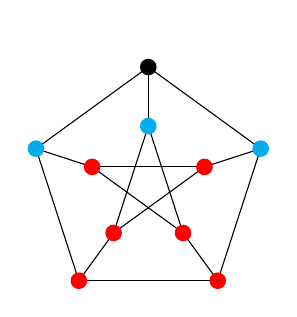
\begin{tikzpicture}
  \coordinate (center) at (1,2);
  \def\radius{.75cm}
  \def\rad2{1.5cm}
  
  \coordinate (o0) at (0*360/5+90:\radius);
  \coordinate (o1) at (1*360/5+90:\radius);
  \coordinate (o2) at (2*360/5+90:\radius);
  \coordinate (o3) at (3*360/5+90:\radius);
  \coordinate (o4) at (4*360/5+90:\radius);

  \coordinate (i0) at (0*360/5+90:\rad2);
  \coordinate (i1) at (1*360/5+90:\rad2);
  \coordinate (i2) at (2*360/5+90:\rad2);
  \coordinate (i3) at (3*360/5+90:\rad2);
  \coordinate (i4) at (4*360/5+90:\rad2);
  
  \draw (i0) -- (i1);
  \draw (i1) -- (i2);
  \draw (i2) -- (i3);
  \draw (i3) -- (i4);
  \draw (i4) -- (i0);
  
  \draw (o0) -- (o2);
  \draw (o0) -- (o3);
  \draw (o1) -- (o3);
  \draw (o1) -- (o4);
  \draw (o2) -- (o4);
   
  \draw (i0) -- (o0);
  \draw (i1) -- (o1);
  \draw (i2) -- (o2);
  \draw (i3) -- (o3);
  \draw (i4) -- (o4);
  
  \fill[cyan] (center) (o0) circle[radius=3pt];
  \fill[red] (center) (o1) circle[radius=3pt];
  \fill[red] (center) (o2) circle[radius=3pt];
  \fill[red] (center) (o3) circle[radius=3pt];
  \fill[red] (center) (o4) circle[radius=3pt];

  \fill[black] (center) (i0) circle[radius=3pt];
  \fill[cyan] (center) (i1) circle[radius=3pt];
  \fill[red] (center) (i2) circle[radius=3pt];
  \fill[red] (center) (i3) circle[radius=3pt];
  \fill[cyan] (center) (i4) circle[radius=3pt];
  
\end{tikzpicture}
\caption{Petersen graph $G$}
%\label{petersen}
\end{subfigure}
\begin{subfigure}{.5\textwidth}
\centering
\begin{tikzpicture}
  \coordinate (v1) at (0,-0.5);
  \coordinate (v2) at (1.5,-0.5);
  \coordinate (v3) at (3,-0.5);
  \coordinate (v3_eps) at (3.25,-0.5);
  \coordinate (loop_label) at (3.65,-0.2);

  \draw (v1) node[below] {$v_1$};
  \draw (v2) node[below] {$v_2$};
  \draw (v3) node[below] {$v_3$};
  
  \draw (v1) -- node[above]{1} (v2);
  \draw (v2) -- node[above]{2} (v3);
  
  \draw (loop_label) node {4};
  
  \draw[black] (v3_eps) circle[radius=6pt];
  
  
  \filldraw[white] (0,1.05) circle[radius=3pt];
  \filldraw[white] (0,-2.1) circle[radius=3pt];
  
  \filldraw[black] (v1) circle[radius=3pt];
  \filldraw[cyan] (v2) circle[radius=3pt];
  \filldraw[red] (v3) circle[radius=3pt];
   
  
%  \[red] (cyan) (o3) circle[radius=3pt];
%  \fill[red] (red) (o3) circle[radius=3pt];
\end{tikzpicture} 
\caption{Graph $G'$}
\label{petersen_a}
\end{subfigure}
\caption{The Petersen graph $G$ and a three vertex weighted graph which it covers.  In the covering map, vertices in $G$ are sent to the vertex with same color in $G'$.\label{petersen}}
\end{figure}

% NOTE(Josh): Can use this later
% \noindent \textbf{Example.}  Consider an even cycle $C_{2n}$, and let $P_{n+1}$
% be the path of length $n+1$.  Then $P_{n+1}$ is a projection of $C_{2n}$.  We
% construct the covering map $\pi$ as follows. 
% 
% 
% Let $d(x,y)$
% be the length of a shortest path from vertex $x$ to vertex $y$ in $C_{2n}$.  
% Denote the vertices of the path by $v_0, v_1, \cdots, v_{n}$, where $v_i$
% is adjacent to $v_{i+1}$.
% Now for any fixed vertex $x$ in $C_{2n}$, we can define the map 
% $\pi : V(C_{2n}) \to V(P_{n+1})$, where $\pi$ sends vertex $y$ to the 
% vertex $v_{d(y,x)}$.  This is a covering map with index $m=2$.  
  
%%%%%%%%%%%%%%%%%%%%%%%%%%%%%%%%%%%%%%%%%%%%%%%%%%%%%%%%%%%%%%%%%%%%%%%%%%
%% SECTION FOUR
%%%%%%%%%%%%%%%%%%%%%%%%%%%%%%%%%%%%%%%%%%%%%%%%%%%%%%%%%%%%%%%%%%%%%%%%%%

\section{Spectral Gap of Graphs in $\mathcal{F}_n$}

\subsection{A Projection of Graphs in $\mathcal{F}_n$}

We begin by constructing a weighted graph $G_n$ on three vertices, which is
a projection of every graph in $\mathcal{F}_n$.  Then we compute the 
eigenvalues of $G_n$, and by Corollary~\ref{cor:cov-cor}, these will be 
eigenvalues of every graph in $\mathcal{F}_n$.  
Let $F$ be a graph in $\mathcal{F}_n$, and 
let $G_n$ be the weighted graph with vertices $\{v_1, v_2, v_3\}$,
with edge weights $w(v_1,v_1) = n-2$, $w(v_1,v_2) = 1$, $w(v_2, v_3) = n-2$,
$w(v_3,v_3) = (n-2)^2$, and all other edge weights zero.
To construct the covering map $\pi : V(F) \to V(G_n)$, we just need to 
specify the sets $U_1 = \pi^{-1}(v_1), U_2 = \pi^{-1}(v_2), U_3 = \pi^{-1}(v_3)$: 
\begin{eqnarray*}
 U_1 = \pi^{-1}(v_1) & = & \{\tau \in S_n : \tau_n = n \} \\
 U_2 = \pi^{-1}(v_2) & = & \{\tau \in S_n : \tau_1 = n \} \\
 U_3 = \pi^{-1}(v_3) & = & \{\tau \in S_n : \tau_1 \neq n, \tau_n \neq n \}  
\end{eqnarray*}


\noindent In order to verify that this is a covering, we need to check the two properties:
\begin{itemize}
\item[(1)]  We need to show that any two vertices in the same preimage set $U_i$ have
  the same number of neighbors in each preimage set $U_j$.  For example, take
  $\tau \in U_3$, so $\tau_k = n$ for some $1 < k < n$.  By definition of
  $\mathcal{F}_n$, if $\sigma$ is adjacent to $\tau$ then either
  $\sigma_n = \tau_n$ or $\sigma_n = \tau_1$.  In particular,
  $\sigma_n \neq n$, so $\tau$ is not adjacent to any vertex in $U_1$.
  There is exactly one neighbor of $\tau$ with $\sigma_1 = n$, and
  so $\tau$ is adjacent to exactly one vertex in $U_1$.  The remaining
  $n-2$ neighbors of $\tau$ are in $U_3$.  As required, the number of neighbors in each
  preimage set did not depend on the choice of $\tau \in U_3$.
  The cases that $\tau \in U_1$ and $\tau \in U_2$ are similar.
 
 \item[(2)]  We need to verify equation~\ref{covering_sum_condition} for each
   pair chosen from the preimage sets $U_1, U_2, U_3$.  
 For this covering, we have $m=(n-1)!$. 
 Firstly, $U_1$ and $U_1$:
  \[ \sum_{\substack{x \in U_1 \\ y \in U_1}} w(x,y) = \sum_{x \in U_1} (n-2)\]
 since each element of $U_1$ is adjacent to exactly $n-2$ elements in $U_1$.
 So 
  \[ \sum_{\substack{x \in U_1 \\ y \in U_1}} w(x,y) = |U_1| (n-2) = (n-1)! w(v_1,v_1)\]
 as required.  The pairs $U_1$, $U_2$ and $U_2$, $U_3$ are similarly verified.
 
% Next, $U_1$ and $U_2$:
 %  \[ \sum_{\substack{x \in U_1 \\ y \in U_2}} w(x,y) = \sum_{x \in U_1} 1 = (n-1)! w(v_1, v_2) .\]
 For the pair $U_1$ and $U_3$, since there are no edges between these sets
and since $w(v_1,v_3) = 0$, we are done.  Similarly for the pair $U_2$ and $U_2$.
 %For $U_2$ and $U_3$ we have 
 %\[\sum_{\substack{x \in U_2 \\ y \in U_3}} w(x,y) = \sum_{x \in U_1} (n-2) = (n-1)! w(v_2, v_3) . \]
 And finally, the pair $U_3, U_3$:
  \[\sum_{\substack{x \in U_3 \\ y \in U_3}} w(x,y) = \sum_{x \in U_3} (n-2) = |U_3|(n-2)\]
 Now  $|U_3| = n! - |U_1| - |U_2| = (n-2) (n-1)!$, so we get
  \[\sum_{\substack{x \in U_3 \\ y \in U_3}} w(x,y)  = (n-1)! w(v_3,v_3)\]
 as required.  
 
\end{itemize}
Now that we have a covering, we evaluate the eigenvalues of the projection $G_n$.

\begin{lemma}
\label{g_eigen}
The eigenvalues of the normalized Laplacian  of $G_n$ are \\$0, \frac 1{n-1}, \frac n {n-1}$.  
\end{lemma}
\begin{proof}
% The adjacency matrix of $G_n$ is 
% \[ \left[ \begin{array}{ccc}  n-2 & 1 & 0\\
%                              1 & 0 & n-2 \\
%                             0 & n-2 &  (n-2)^2
%                              \end{array} \right] \]
The normalized Laplacian of $G_n$ is
                              \[ \left[ \begin{array}{ccc}  \frac 1 {n-1} &- \frac 1 {n-1} & 0\\
                             - \frac 1 {n-1} &1 &- \frac{\sqrt{n-2}}{n-1} \\
                             0 &  -\frac{\sqrt{n-2}}{n-1} &  \frac 1 {n-1}
                              \end{array} \right] \]
 The result follows from a simple computation.
\end{proof}

\begin{corollary}\label{cor:adj_spec}
For any $G \in \mathcal{F}_n$, the adjacency matrix $A_{G}$ has eigenvalues $n-1$, $n-2$ and $-1$.
For $1 \leq i \leq n$ define
\begin{eqnarray*}
 X(i) & = & \{\tau \in S_n : \tau_n = i \} \\
 Y(i) & = & \{\tau \in S_n : \tau_1 = i \} \\
 Z(i) & = & \{\tau \in S_n : \tau_1 \neq i, \tau_n \neq i \}  
\end{eqnarray*}
Then any eigenfunction corresponding to any other eigenvalue than those listed above must sum to zero on
each of $X(i)$, $Y(i)$ and $Z(i)$, for any $i \in \{1,2,\cdots,n\}$.
\end{corollary}
\begin{proof}
  When defining the covering mapping $\pi$ to $G_n$, for
  a permutation $\tau$ the vertex it was mapped to was
  determined by the position of $n$ in $\tau$. 
  Observe that we can replace $n$ with any index $i$, $1 \leq i \leq n$, and
  we still have a covering, in this case with preimage sets $X(i)$, $Y(i)$, $Z(i)$.


  Now take an eigenfunction of $G$ which corresponds to an eigenfunction other than
  $n-1$, $n-2$, or $-1$.  $G$ is regular, so this eigenfunction is also an
  eigenfunction of the normalized Laplacian of $G$, corresponding to an eigenvalue
  other than $0$, $1/(n-1)$ or $n/(n-1)$.  It follows from Corollary~\ref{cor:cov-cor}
  and the previous lemma that the eigenfunction must sum to zero over the preimage
  sets of the covering, which are $X(i)$, $Y(i)$ and $Z(i)$.    
\end{proof}

%%%%%%%%%%%%%%%%%%%%%%%%%%%%%%%%%%%%%%%%%%%%%%%%%%%%%%%%%%%%%%%%%%%%%%%%%%
%% SECTION FIVE
%%%%%%%%%%%%%%%%%%%%%%%%%%%%%%%%%%%%%%%%%%%%%%%%%%%%%%%%%%%%%%%%%%%%%%%%%%


\subsection{The Spectral Gap is $1$}

Recall that $\mathcal{F}_n$ is the family of graphs whose vertex set is $S_n$ and
where for each vertex $\tau$,
\[ \tau = (\tau_1, \tau_2, \cdots, \tau_n), \]
and each $2 \leq i \leq n$, $\tau$ is adjacent to exactly one vertex of the form 
\[ (\tau_i, \alpha_2, \alpha_3, \cdots, \alpha_{i-1}, \tau_1, \tau_{i+1}, \cdots, \tau_n). \]
Each graph in $\mathcal{F}_n$ is an $(n-1)$-regular graph.  The prefix reversal graph $\mathcal{P}_n$
is in $\mathcal{F}_n$, as well as the right-Cayley graph generated by the transpositions $(1\ k)$,
where $2 \leq k \leq n$.


In order to compute the spectral gap of graphs in $\mathcal{F}_n$, we proceed
by induction, so first we compute the spectrum of graphs in $\mathcal{F}_3$ to 
establish our base case.  

\begin{lemma}\label{base_case}
  $\mathcal{F}_3 = \{ C_6 \}$.  In particular, the adjacency spectral gap of every graph in
  $\mathcal{F}_3$ is one.
\end{lemma}
\begin{proof}
  Let $G \in \mathcal{F}_3$.  Then $G$ is a $2$-regular graph on $3! = 6$ vertices.
  From the definition of $\mathcal{F}_3$, it is easy to verify that $G$ is connected,
  and so $G = C_6$.  The first two adjacency eigenvalues of $C_6$ are $2$ and $1$.
\end{proof}

%\begin{theorem}
%  For $n \geq 3$, and any $G \in \mathbb{P}_n$, the spectral gap of $\mathcal{L}_{G}$ is $1/(n-1)$, and the spectral
%  gap of $A_{G}$ is $1$.

We can now prove the  theorem on the spectral gap of ${\mathcal F}_n$, as stated in the Section~1.

%\end{theorem}
\begin{proof}[Proof of Theorem~\ref{thm:main}]
  We proceed by induction,
  so assume that the adjacency spectral gap of any graph in $\mathcal{F}_{n-1}$ is $1$.  
  The base case is established by Lemma~\ref{base_case}.  By $(n-2)$-regularity of graphs
  in $\mathcal{F}_{n-1}$, it follows from the inductive assumption that the second largest
  eigenvalue of any graph in $\mathcal{F}_{n-1}$ is $n-3$.


  Let $G$ be a graph in $\mathcal{F}_{n}$.
  Pick any eigenvector $f$ coming from an eigenvalue $\lambda$ that is not
  $n-1$, $n-2$ or $-1$.  Our goal is to show that $\lambda < n-2$.
  Recall that $X(i)$ consists of the permutations whose 
  last entry is $i$, $Y(i)$ consists of the permutations whose first entry is
  $i$ and $Z(i)$ consists of all other permutations.  For any $i$, from 
  Corollary~\ref{cor:adj_spec}
  we get a projection of $G$ with preimage sets 
  $X(i), Y(i), Z(i)$.
  The set $X(i)$ induces a graph in $\mathcal{F}_{n-1}$, and the set $Y(i)$
  induces an independent set (since every two adjacent permutations have
  different first entries).
  Furthermore the edges between $X(i)$ and 
  $Y(i)$ form a matching.  Our proof strategy is the following:  we will
  get an expression for $\lambda$ involving the values of $f$ on the 
  set $X(i)$ and the set $Y(i)$.  We can control the contribution from 
  $X(i)$ using the inductive assumption, and then we show that we can
  choose $i$ so that the contribution from $Y(i)$ is small enough
  to yield the stated result.
  
  
  \vspace*{1mm}
  \noindent \textbf{Claim:} We can fix an $i$ such that 
   \begin{equation}\label{eqn:gap_max}
     \sum_{x \in X(i)} f(x)^2 \geq \sum_{y \in Y(i)} f(y)^2
   \end{equation}
   and 
   \[ \sum_{x \in X(i)} f(x)^2 > 0. \]
   \textbf{Proof of claim:} Notice that the sets $X(1), X(2), \cdots, X(n)$
  partition the vertex set of $G$ (ie.  partitioning the permutations
  based on the last entry).  Similarly, the sets 
  $Y(1), Y(2), \cdots, Y(n)$ partition the vertex set of $G$.
  Hence
   \[ \sum_{j=1}^n \sum_{x \in X(j)} f(x)^2 = \sum_{j=1}^n \sum_{y \in Y(j)} f(y)^2 >0 . \]
  In particular, there exists an index $i$ such that 
   \begin{equation*}
     \sum_{x \in X(i)} f(x)^2 \geq \sum_{y \in Y(i)} f(y)^2.
   \end{equation*}
Let $I$  denote the set of indices $i$ satisfying the above inequality. Then there exists some $i$ in $I$ satisfying
   \begin{equation*}
     \sum_{x \in X(i)} f(x)^2 > 0
   \end{equation*}
  since $f \not = 0$. This proves the claim.
  
  
  
  Consider an arbitrary vertex $x \in X(i)$.  Then by
  definition of $X(i)$, $x$
  is a permutation with $x(n) = i$.
  $x$ has $n-1$ neighbors in $G$, $n-2$ of these neighbors
  are in $X(i)$ and one of its neighbors is in $Y(i)$.
  Let $c_x$ be the unique neighbor of $x$ in $Y(i)$.
  As noted above, the induced subgraph on $X(i)$ is in $\mathcal{F}_{n-1}$.
  By the eigenvalue-eigenvector equation, we have
   \[ \lambda f(x) = f(c_x) + \sum_{y \in N(x) \cap X(i)} f(y) .\]
  Multiplying both sides by $f(x)$, and summing over $x \in X(i)$
  yields
   \[ \lambda \sum_{x \in X(i)} f(x)^2 = \sum_{x \in X(i)} f(x) f(c_x) + \sum_{x \in X(i)} \sum_{y \in N(x) \cap X(i)} f(x) f(y) .\]
  Dividing across by the sum on the left-hand side (which is non-zero 
  by our claim above) gives
   \begin{equation}\label{eqn:gap_to_bound}
     \lambda = \frac{\sum_{x \in X(i)} f(x) f(c_x)}{\sum_{x \in X(i)} f(x)^2} + \frac{\sum_{x \in X(i)} \sum_{y \in N(x) \cap X(i)} f(x) f(y)}{\sum_{x \in X(i)} f(x)^2} .
    \end{equation}
  We will now find upper bounds for each of the two terms on
  the right-hand side.
  
  Let ${G'}$ be the induced subgraph on $X(i)$, which is a graph in $\mathcal{F}_{n-1}$, and let
  $g = f|_{X(i)}$.
  Since $\sum_{x \in X(i)} f(x)=0$, we have that $g \perp \textbf{1}$, where $\textbf{1}$ is the constant vector with entries $1$,
  which is the eigenvector associated with $\lambda_1$.
  Now we can bound the second term in equation~\ref{eqn:gap_to_bound} by $n-3$:
     \begin{eqnarray*}
     \displaystyle \frac{\displaystyle\sum_{x \in X(i)} \displaystyle\sum_{y \in N(x) \cap X(i)} f(x) f(y)}{\displaystyle\sum_{x \in X(i)} f(x)^2} & = & \frac{g^T A_{G'} g}{ g^T g} \\
     &\leq& \text{max}_{h \perp \textbf{1}} \frac{h^T A_{G'} h}{h^T h} \\
     &=& \lambda_2(G') \\
     &=& n-3.
   \end{eqnarray*}
 
 



   The edges between $X(i)$ and $Y(i)$ are a matching.
  So as $x$ ranges over the vertices of $X(i)$, $c_x$ ranges over
  the vertices of $Y(i)$.  By Cauchy--Schwarz,
   \begin{eqnarray*} 
   \sum_{x \in X(i)}f(x) f(c_x) & \leq & \sqrt{\sum_{x \in X(i)}f(x)^2 \sum_{x \in X(i)}f(c_x)^2 } \\
   & = & \sqrt{\sum_{x \in X(i)}f(x)^2 \sum_{y \in Y(i)}f(y)^2 } 
   \end{eqnarray*}
  So
   \[ \frac{\displaystyle \sum_{x \in X(i)} f(x) f(c_x)}{\displaystyle \sum_{x \in X(i)} f(x)^2} \leq \sqrt{\frac{\displaystyle \sum_{y \in Y(i)}f(y)^2}{\displaystyle {\sum_{x \in X(i)}f(x)^2}}} \leq 1 \]
  where the last inequality follows from equation~\ref{eqn:gap_max}.
   
  Applying these two bounds in equation~\ref{eqn:gap_to_bound} gives
  \[ \lambda \leq n-3 + 1 = n-2 . \]
  This shows that there is no eigenvalue of $G$ strictly between $n-2$ and $n-1$, so
  we conclude that  $\lambda_2(G) = n-2$.
\end{proof}


As a brief application of Theorem~\ref{thm:main}, we can establish bounds on the edge
expansion of every graph in $G \in \mathcal{F}_n$.  Recall that the edge
expansion of a $d$-regular graph $G$, $h_G$, is defined as
\[ h_G = \min_{S \subset V(G)} \frac{|E(S,\bar{S})|}{\min(|S|,|\bar{S}|) \cdot d} .\]
If $S$ is the set of permutations whose last entry is $n$, then
$|S| = |E(S,\bar{S})| = (n-1)!$, which gives the upper bound
$h_G \leq 1/(n-1)$.  To obtain a lower bound, we can use an inequality
from \cite{Chung1997},
$h_G \geq \mu_1 / 2$.   Combining these two inequalities gives the bounds
 \[ \frac{1}{2(n-1)} \leq h_G \leq \frac{1}{n-1} .\] 


%%%%%%%%%%%%%%%%%%%%%%%%%%%%%%%%%%%%%%%%%%%%%%%%%%%%%%%%%%%%%%%%%%%%%%%%%%
%% SECTION SIX
%%%%%%%%%%%%%%%%%%%%%%%%%%%%%%%%%%%%%%%%%%%%%%%%%%%%%%%%%%%%%%%%%%%%%%%%%%

\section{The Reversal Graph}\label{s6}

\subsection{A Graph Projection of the Reversal Graph}

The graph $R_n$ is a Cayley graph of $S_n$ that does not
belong to the family $\mathcal{F}_n$ but is closely related.  For any 
$1 \leq i<j \leq n$, let $r_{i,j}$ denote the bijection on $S_n$
defined by
 \[ r_{i,j}(\tau) =  (\tau_1, \tau_2, \cdots, \tau_{i-1}, \tau_{j}, \tau_{j-1}, \cdots \tau_{i+1}, \tau_i, \tau_{j+1}, \cdots , \tau_{n})\] 
That is, it reverses the subsequence from indices $i$ to $j$, inclusive.
Then two permutations $\sigma$ 
and $\tau$ are adjacent in $R_n$ iff $\tau = r_{i,j}(\sigma)$ for some $i< j$.  We will first  show that $R_n$ has many integer eigenvalues.  We remark that the spectrum of $R_n$ is not generally
integer-valued, despite the presence of many integer eigenvalues.  A plot of
the $7!$ eigenvalues of $R_7$ is given in Figure~\ref{fig-spec7}.  We will first prove the following useful fact.


\begin{figure}[h]
\begin{center}
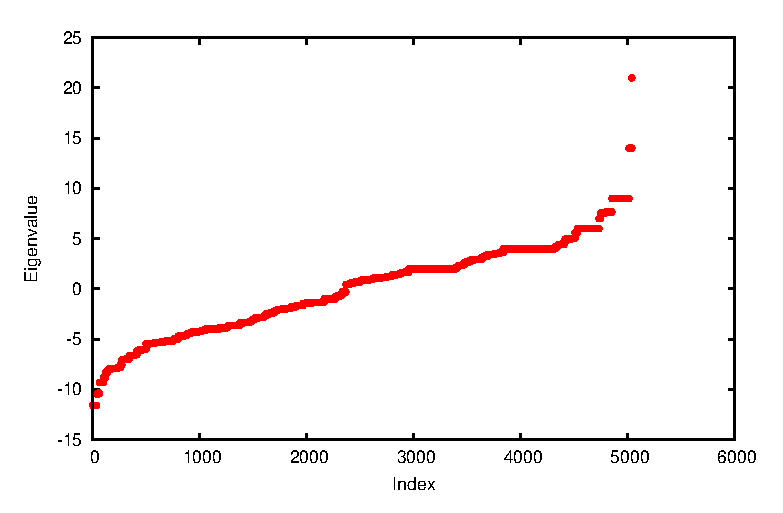
\includegraphics[scale=.85]{figures/all_spec7.eps} 
\end{center}
\caption{The adjacency eigenvalues of the reversal graph, $R_7$, plotted in increasing order.
  \label{fig-spec7}}
\end{figure}


\begin{lemma}\label{lem:rev_eig}
Let $X$ be the symmetric $n \times n$ matrix with entries
 \[ X_{i,j} = \text{min} \left\{ i,j,n+1-i,n+1-j \right\} \]
For a given real number $x$, let $D$ be the unique diagonal matrix such 
that every row of $D+X$ sums to $x$.  Then the eigenvalues of $D+X$ are
\[ \lambda_k =  x - \left\lfloor \frac{k}{2} \right\rfloor n + 2 \binom{\left \lfloor \frac{k}{2} \right \rfloor}{2}, 1 \leq k \leq n . \]
In particular, $\lambda_1 = x$, $\lambda_2 = x-n$.
%   \[x, x-n, x - n - (n-2),  \cdots, x - n - (n-2) - \cdots - \left(n - 2 \left\lfloor \frac{n}{2} \right\rfloor\right)\]
\end{lemma}


\noindent \textbf{Example: } For $n=5$ and $x=12$ we get
\[ D+X = \begin{pmatrix}
 7 & 0 & 0 & 0 & 0 \\
 0 & 4 & 0 & 0 & 0 \\
 0 & 0 & 3 & 0 & 0 \\
 0 & 0 & 0 & 4 & 0 \\
 0 & 0 & 0 & 0 & 7 
\end{pmatrix}
+ \begin{pmatrix}
 1 & 1 & 1 & 1 & 1 \\
 1 & 2 & 2 & 2 & 1 \\
 1 & 2 & 3 & 2 & 1 \\
 1 & 2 & 2 & 2 & 1 \\
 1 & 1 & 1 & 1 & 1 
\end{pmatrix} \]
which has eigenvalues $12, 7, 7, 4, 4$.


\begin{proof}
 We proceed by induction.  For the case $n=1$, the result is immediate.  
 When $n=2$, we have
  \[ D+X = \begin{pmatrix}
 x-1 & 1 \\
 1 & x-1
\end{pmatrix} \]
which has eigenvalues $x$ and $x-2$, as required.

Now fix $n$ and assume the result holds for all smaller dimensions. 
Since $D+X$ is a symmetric matrix with constant row sums, the leading 
eigenvector of $D+X$ is
the all-ones vector $\textbf{1}$, with corresponding eigenvalue 
$x$.  All other eigenvectors are orthogonal to $\textbf{1}$.
It follows that if $Y = D+X - \textbf{1}\textbf{1}^T$,
then $D+X$ and $Y$ have the same eigenvectors.   Moreover, 
the spectrum of $Y$, counting multiplicity, is exactly the
spectrum of $D+X$ with $x$ replaced by $x-n$.


The only non-zero entry in the top row of $Y$ is the top-left entry, which
is $x-n$.  The only non-zero entry in the bottom row of $Y$ is the bottom-right entry which is also $x-n$.
Denote the characteristic polynomial of a matrix $A$ by $p_A(\lambda)$.  Expanding the determinant of $Y - \lambda I$
along the top row and then along the bottom row, we obtain that 
 \[ p_Y(\lambda) = (\lambda - x + n)^2 p_{Y'}(\lambda) \]
where $Y'$ is the $(n-2) \times (n-2)$ principal submatrix of $Y$, obtained
by deleting the first and last rows and columns.  In particular, the spectrum
of $Y$ consists of $x-n$ with multiplicity two, and the spectrum of $Y'$.
Hence, from the relationship between the spectrum of $D+X$ and the spectrum of
$Y$ discussed above, we  have that the eigenvalues of $D+X$ are exactly
the eigenvalues of $Y'$, together with $x$ and $x-n$.


Observe that $Y'$ satisfies the conditions of the theorem, with row sum equal 
to $x-n$.  By induction, we have that the eigenvalues of $Y'$ are (for $1 \leq k \leq n-2$):
\begin{eqnarray*}
  \lambda_k(Y') & = & (x-n) - \left\lfloor \frac{k}{2} \right\rfloor (n-2) + 2 \binom{\left\lfloor \frac{k}{2} \right\rfloor}{2} \\
  & = & x - \left\lfloor \frac{k+2}{2} \right\rfloor n + 2 \binom{\left\lfloor \frac{k+2}{2} \right\rfloor}{2} .
\end{eqnarray*}
Combining these $n-2$ eigenvalues with $x$ and $x-n$ yields exactly the claimed spectrum for $D+X$.
\end{proof}

\begin{lemma}\label{lem:rev_eig2}
  The spectrum of the adjacency matrix of the reversal graph, $A_{R_n}$, 
  contains the eigenvalues
\[ \lambda_k =  \binom{n}{2} - \left\lfloor \frac{k}{2} \right\rfloor n + 2 \binom{\left \lfloor \frac{k}{2} \right \rfloor}{2}, 1 \leq k \leq n . \]
%   \[\binom{n}{2}, \binom{n}{2}-n, \binom{n}{2} - n - (n-2),  \cdots, \binom{n}{2} - n - (n-2) - \cdots - \left(n - 2 \left\lfloor \frac{n}{2} \right\rfloor\right)\]
  In particular, $\binom{n}{2}$ and $\binom{n}{2} - n$ are eigenvalues, and so the spectral gap is at most $n$. 
\end{lemma}  

\begin{proof}
  We begin by constructing a projection of the graph $R_n$.
  Let $G$ be the graph with vertices $v_1$, $v_2$, $\cdots$,
  $v_n$ corresponding to the adjacency matrix $A_G = D+X$,
  where vertex $v_i$ corresponds to row and column $i$, and
  $D+X$ is as in the previous lemma, with row sum $\binom{n}{2}$.
  Let $U(i)$ be the set of all permutations $\tau$ such that $\tau_i = n$.
  The sets $U(i)$, for $1\leq i \leq n$, partition $V(R_n)$, so we
  can define a map $\pi : V(R_n) \to V(G)$ by
  setting $\pi(x) = v_i$ whenever $x \in U(i)$.  It suffices to show
  that this is a covering map, then the result will follow
  from the previous lemma.


  To show that $\pi$ satisfies the first property of a graph cover,
  we need that for all indices $i,j$, any two vertices in $U(i)$
  have the same number of neighbors in $U(j)$.  This follows from the
  fact that there are a fixed number of reversals that map
  entry $i$ to entry $j$.

%  Firstly,
%  assume that $i < j$.  Then the reversals that map
%  a vertex in $U(i)$ to $U(j)$ are exactly
%  $r_{i,j}, r_{i-1,j+1}, r_{i-2,j+2}, \cdots$.  It follows that
%  any vertex in $U(i)$ is adjacent to exactly
%  $\text{min}\left\{i,j,n+1-i,n+1-j\right\}$ vertices in $U(j)$.
%  Similarly if $j < i$.
%  Secondly, assume $i = j$.  For any vertex in $U(i)$,
%  there are several types of reversals that map it back into $U(i)$:
%  the reversals $r_{j,k}$ where $j < k < i$; the reversals 
%  $r_{j,k}$ where  $i < j < k$; and finally the reversals of the form
%  $r_{i-k,i+k}$.  In every case, all vertices in $U(i)$ have
%  the same number of neighbors in $U(j)$.


  For the second property, take two preimage sets $U(i)$, $U(j)$,
  and $\tau_0$ some permutation in $U(j)$.  It is easily checked
  that by construction of the weighted graph $G$, we have
  \[ w(v_i, v_j) = \left| N(\tau_0) \cap U(i) \right| .\]
  Then
  \begin{eqnarray*}
    \displaystyle \sum_{\sigma \in U(i)} \sum_{\tau \in U(j)} w(\sigma,\tau) & = & \sum_{\sigma \in U(i)} |U(j)| w(\sigma,\tau_0) \\
    & = & (n-1)! \left| N(\tau_0) \cap U(i) \right|  \\
    & = & (n-1)! w(v_i, v_j)
  \end{eqnarray*}
  where the first equality follows from property (i).
  Hence $\pi$ is a covering with $m = (n-1)!$.

  %CURP
  
%  Consider a vertex $\tau$ in 
%$U(i)$, and any index $j > i$.  The reversals that map $\tau$ into 
%$U(j)$ are exactly $r_{i,j}, r_{i-1,j+1}, r_{i-2,j+2}, \cdots$.   It
%follows that the  number of vertices in $U(j)$ that are adjacent 
%to $\tau$ is $\text{min}\left\{i,j,n+1-i,n+1-j\right\}$.  This is independent
%of the vertex $\tau$ chosen.  Similarly, we get the same total
%when $j < i$.  In particular any two vertices in $U(i)$
%have the same number of neighbors in $U(j)$, for any $j \neq i$.  
%
%There are several types of reversals that map $\tau$ back into $U(i)$.  They
%are: the reversals $r_{j,k}$ where $j < k < i$, the reversals 
%$r_{j,k}$ where  $i < j < k$, and finally the reversals of the form
%$r_{i-k,i+k}$.  Again, the number of such reversals does not depend on the 
%vertex $\tau$ chosen, and so any two vertices in $U(i)$ have the same number
%of neighbors in $U(i)$.  
%
%
%It follows from the above two paragraphs that we can form a projection of 
%the graph $R_n$ on $n$ vertices, with preimage sets $U(i)$.  The 
%adjacency matrix of this projection can be written as $D+X$, where 
% \[ X(i,j) = \text{min}\left\{i,j,n+1-i,n+1-j\right\} \] 
%and $D$ is the unique diagonal such that $D+X$ has constant row sum equal
%to $\binom{n}{2}$.  By Corollary~\ref{cor:cov-cor}, the eigenvalues
%of $D+X$ are eigenvalues of $A_{R_n}$.  The result then follows from 
%Lemma~\ref{lem:rev_eig}.
\end{proof}

\subsection{The Spectral Gap of the Reversal Graph}

We are finally ready to prove the main theorem determining the spectral gap of $R_n$.

\noindent
{\it Proof of Theorem \ref{thm:rev_eig}:}
 The value of $\lambda_1$ is $\binom n 2$ since $R_n$ is regular of degree $\binom n 2$.   
 From the previous lemma we have that 
  \[ \lambda_2 \geq \binom{n}{2} - n\]
 so it suffices to prove that
  \[ \lambda_2 \leq \binom{n}{2} - n .\]
 We follow a similar approach to the proof of 
 Theorem~\ref{thm:main}.  
 
 
 We proceed by induction.  For the base case, consider $n=2$.  Then $R_2$
 is $K_2$, with eigenvalues $1,-1$.  Now assume for any $m < n$, we have
 \[  \lambda_2(A_{R_m}) = \binom{m}{2} - m . \]
 For any $1 \leq i \leq n$, we define the sets
  \[ U_i(j) = \left\{ \tau \in S_n : \tau_j = i \right\}. \]
 As in the proof of Lemma~\ref{lem:rev_eig2}, for any fixed $i$ the sets 
 $U_i(j)$, $1 \leq j \leq n$ are the preimages of a covering map of $R_n$,
 and the two largest eigenvalues of the projection are $\binom{n}{2}$ and
 $\binom{n}{2} - n$.  It follows from Corollary~\ref{cor:cov-cor}
 that if $A_{R_n}$ has an eigenvalue $\lambda$ strictly between $\binom{n}{2}$
 and $\binom{n}{2} - n$ then the corresponding eigenvector must sum to zero
 on $U_i(j)$ for all $i,j$.  Let $\lambda$ be such an eigenvalue, with 
 eigenvector $f$.
 
 
 Let $E_1 = \left\{ \left\{\sigma, \tau\right\} \in E(R_n) : \sigma_1 \neq \tau_1 \right\}$,
 that is, the set of edges arising from substring reversals that include 
 the first entry of the permutation.  Observe that the edge set $E_1$
 is exactly the set of edges of the prefix reversal graph $\mathcal{P}_n$.
 Let $R'$ be the graph obtained by removing all edges in $E_1$ from $R_n$.  Then
 $R'$ consists of $n$ connected components, $U_1(1), U_2(1), \cdots, U_n(1)$.
 Each of these connected components is isomorphic to $R_{n-1}$.  
 
 
We have, by the Rayleigh quotient
  \begin{eqnarray*}
   \lambda & = &  \frac{2\sum_{\{x,y\} \in E(R_n)} f(x) f(y)}{\sum_{x \in R_n} f(x)^2}\\
   & = & \frac{2\sum_{\{x,y\} \in E_1} f(x) f(y)}{\sum_{x \in R_n} f(x)^2} + \frac{2\sum_{\{x,y\} \not \in E_1} f(x)f(y)}{\sum_{x \in R_n} f(x)^2}\\
   & \leq & \lambda_2(A_{\mathcal{P}_n}) + \frac{2\sum_{\{x,y\} \not \in E_1} f(x) f(y)}{\sum_{x \in R_n} f(x)^2}
   \end{eqnarray*}
 where the last inequality follows since $f$ is orthogonal to the constant
 vector $\textbf{1}$.  Using Theorem~\ref{thm:main} we have 
 $\lambda_2(A_{\mathcal{P}_n}) = n-2$.
 
 
 To bound the second term, we will partition the edges not in $E_1$ in the following way
  \[ \left\{ \left\{ x,y \right\} \not \in E_1 \right\} = E(U_1(1)) \cup E(U_2(1)) \cup \cdots \cup E(U_n(1)) . \]
 Hence, we have 
  \begin{eqnarray*}
   \frac{2\sum_{\{x,y\} \not \in E_1} f(x) f(y)}{\sum_{x \in R_n} f(x)^2} & = & 
   \frac{\sum_{i=1}^n 2\sum_{\{x,y\} \in E(U_i(1))} f(x) f(y)}{\sum_{i=1}^n \sum_{x \in U_i(1)} f(x)^2} \\
   & \leq & \text{max}_{1 \leq i \leq n}  \frac{2\sum_{\{x,y\} \in E(U_i(1))} f(x) f(y)}{\sum_{x \in U_i(1)} f(x)^2} \\
   & \leq & \lambda_2(A_{R_{n-1}}) 
  \end{eqnarray*}
 where we are using the fact that $v$ sums to zero over each set $U_i(1)$.
 Combining the two inequalities above, we get 
  \begin{eqnarray*}
  \lambda & \leq & \lambda_2(A_{\mathcal{P}_n}) + \lambda_2(A_{R_{n-1}}) \\
  & = & (n-2) + \binom{n-1}{2} - (n-1) \\
  & = & \binom{n}{2} - n
  \end{eqnarray*}
  Thus we conclude that $\lambda_2(A_{R_n}) = \binom n 2 -n$ and this completes the proof of Theorem \ref{thm:rev_eig}.
\qed



%%%%%%%%%%%%%%%%%%%%%%%%%%%%%%%%%%%%%%%%%%%%%%%%%%%%%%%%%%%%%%%%%%%%%%%%%%
%% SECTION SEVEN
%%%%%%%%%%%%%%%%%%%%%%%%%%%%%%%%%%%%%%%%%%%%%%%%%%%%%%%%%%%%%%%%%%%%%%%%%%

\section{Future Work}
Consider the stochastic process of pancake flipping:  Start with a stack of $n$ pancakes (or $n$ cards). At each
step, with probability $1/n$,  choose $i$ where $i=1, \ldots, n$ and  do a pancake flipping of the first $i$ pancakes. 
The above process is equivalent to taking a random walk on 
$\mathcal{P}_n + I$, where $\mathcal{P}_n$ is the pancake graph. The transition probability 
matrix is then $P=(A(\mathcal{P}_n)+I)/n$.

Since the first nontrivial eigenvalue of the normalized Laplacian of $\mathcal{P}_n$ is $1/(n-1)$. Consequently,
the first nontrivial eigenvalue of
the normalized Laplacian of $\mathcal{P}_n + I$ is $1/n$ and all eigenvalues of the normalized Laplacian
of $\mathcal{P}_n + I$ are at most $2-1/n$. It is known that the rate of convergence for random walk is the inverse of  $\mu^{-1}$ where $\mu= \min \{\mu_1, 2-\mu_{n-1}\}$ where $0=\mu_0,
\mu_1, \ldots, \mu_{n-1}$ are the nontrivial eigenvalues of the normalized Laplacian of $\mathcal{P}_n + I$. However, in order to get tight bounds for the convergence of the random walk to the stationary distribution under the  total variational distance, more work is needed. For a vertex-transitive graph, a general upper bound after $t$ steps of random walk on 
$\mathcal{P}_n + I$ can be derived by using the Plancherel formula (see \cite{Chung1997}):
\begin{align*}
\Delta_{TV}(t) &\leq \frac 1 2 \Big( \sum_{i \not = 0} (1-\mu_i)^{2t}\Big)^{1/2}.
\end{align*}
Using the result that $|1-\mu_i| \leq 1-1/n$ for $i \not = 0$, we have
\begin{align*}
\Delta_{TV}(t) &< \frac 1 2 \Big(1-\frac 1 n\Big)^t n!\\
&\leq e^{-t/n+n \log n}.
\end{align*}
Hence, the random walk converges to the uniform distribution with $\Delta_{TV}(t) \leq e^{-c}$ after at most $t=n^2 \log n + c n$ steps.
If we know more about the distribution of eigenvalues $\mu_i$, this upper bound should be improved.
It seems reasonable to conjecture that $O(n \log n)$ steps suffice.


Similarly, we can consider the random substring reversal process, where in each
step, with probability $\binom{n+1}{2}^{-1}$ we choose a substring (allowing substrings of length $1$) and reverse it.
This is equivalent to taking a random walk on $R_n+ nI$. 
In this case, we have $\mu_1 = n/ \binom {n+1} 2= 2 (n+1)^{-1}$ and $\mu_{n-1} \leq 2  - 2 (n+1)^{-1}$.   As in the case of 
pancake flipping, knowing the spectral gap allows us to obtain a bound on
the rate of convergence, but to obtain sharp bounds it would be desirable to
know more about the distribution of all eigenvalues.

We have mainly focused on substring reversal and pancake flipping on permutations. There are many
interesting variations of these problems. In particular, for applications such as genome
rearrangement, the objects of interest are signed permutations.  In this case the operation of
substring reversal is taking the reverse of the substring and changing the signs of every element in
the substring.  The corresponding problem for pancake flipping is the {\it burnt} pancake problem
where the sign is used to distinguish the two sides of each pancake.  The burnt pancake graph
$\bar{\mathcal P}_n$ has $2^n n!$ vertices and degree $n$.  A natural question is to determine
the spectral gap of the adjacency matrix.  In fact, $\mathcal{P}_n + I$ is a projection of
$\bar{\mathcal{P}}_n$, which implies that the adjacency spectral gap of $\bar{\mathcal{P}}_n$ is
at least one.  A natural guess is that the spectral gap of the adjacency matrix of
$\bar{\mathcal P}_n$ is exactly $1$. However, this
turns out to be not true. For $\bar{\mathcal P}_4$ the spectral gap is approximately $0.71343$,
and for $\bar{\mathcal P}_5$ the spectral gap is approximately $0.75758$.  



This chapter is based on the paper ``The Spectral Gap of Graphs Arising from Substring Reversals'',
submitted to \textit{Journal of Combinatorics}, written jointly with Fan Chung.  The dissertation
author was the primary investigator and author of the paper.


%% APPENDIX
%\appendix
%\chapter{Final notes}
%What to do about things \cite{Martin_1983}.  What did he say \cite{Rilling_Insel_1999}.
%Remove me in case of abdominal pain.



%% END MATTER
% \printindex %% Uncomment to display the index
% \nocite{}  %% Put any references that you want to include in the bib 
%               but haven't cited in the braces.
\bibliographystyle{acm}  %% This is just my personal favorite style. 
%                              There are many others.
%\setlength{\bibleftmargin}{0.25in}  % indent each item
%\setlength{\bibindent}{-\bibleftmargin}  % unindent the first line
%\def\baselinestretch{1.0}  % force single spacing
%\setlength{\bibitemsep}{0.16in}  % add extra space between items
\bibliography{thesis}  %% This looks for the bibliography in template.bib 
%                          which should be formatted as a bibtex file.
%                          and needs to be separately compiled into a bbl file.
\end{document}

